\documentclass[12pt,english]{report}
\usepackage{WSU}
\usepackage[T1]{fontenc}
\usepackage{xcolor}
\usepackage{booktabs} % used for tables
\usepackage{multirow} % used for tables to merge multiple rows
\usepackage{bigdelim} % used for tables to set spacing
\usepackage{bigstrut} % used for tables to set spacing
\usepackage{graphicx} % used for includegraphics
%\usepackage{subfigure} % allows the use of 339
%\usepackage{subfig}

\usepackage{dirtytalk} % for quoation
\usepackage{epstopdf}  %for eps
\usepackage{floatrow}

%% front pages
    
\usepackage[framed,numbered,autolinebreaks,useliterate]{mcode}%used to insert
%code
\usepackage{geometry,array,float,caption,tabularx}
\usepackage{url}
\usepackage{rotating} % for sidewaystable
\usepackage{pdflscape} % for sideway figure
\usepackage{comment}

\usepackage[flushleft]{threeparttable} % add note to table
\usepackage{epstopdf}  %for eps
\usepackage{amsmath}
\usepackage{natbib}  % for citation
\usepackage{verbatim} 

\usepackage{hyperref}

\usepackage{caption}
\usepackage{subcaption}
%\captionsetup{compatibility=false}
    
\usepackage{floatrow}
\newfloatcommand{capbtabbox}{table}[][\FBwidth]
\usepackage{blindtext}

    
\usepackage{verbatim} 
\usepackage{paralist} % for inline list

\setcitestyle{authoryear,open={(},close={)}}
\usepackage{setspace}

\usepackage{adjustbox} 

\begin{comment}

\usepackage{hyperref}

%\usepackage{indentfirst}
% sub section 
%\setcounter{section}{-1}
%\usepackage{titlesec}  % set subsubsubsub section
\setcounter{secnumdepth}{5} % set subsubsubsub section
%\usepackage{listings} % insert code

%\titleformat{\paragraph}
%{\normalfont\normalsize\bfseries}{\theparagraph}{1em}{}
%\titlespacing*{\paragraph}{0pt}{3.25ex plus 1ex minus .2ex}{1.5ex plus .2ex}
\usepackage{array,tabularx,float}
\setlength\extrarowheight{2pt}
\usepackage[nottoc]{tocbibind} % This add reference page number to
tableofcontents


\setcounter{tocdepth}{2}
%level -1: part, 0: chapter, 1: section, etc.
\end{comment}

%-----------------------------------------------------------------------
%  Modified fields
%-----------------------------------------------------------------------%
%\begin{comment}

\newcommand{\authorfirst}{Shuai}
\newcommand{\authorMI}{}
\newcommand{\authorlast}{Wang}
\newcommand{\degreefull}{Doctor of Philosophy}  
\newcommand{\degreeshort}{Ph.D in Engineering Program}
\newcommand{\thesisordissertationlc}{Dissertation}
\newcommand{\dept}{Department of Biomedical, Industrial and Human Factors
Engineering}
\newcommand{\institution}{Wright State University}
% \newcommand{\thesisordissertationlc}{thesis}%
\newcommand{\thesistitle}{Data Mining Techniques and Mathematical Models for
the Optimal Scholarship Allocation Problem for a State University}
\newcommand{\bachdegreeshort}{B.S., Management} % Bachelor degree short
\newcommand{\bachinstitution}{Dalian Jiaotong University} % Bachelor degree

\newcommand{\bachyear}{2011}% Bachelor degree year
%No spaces should be before or after this title.
\newcommand{\pdfsubject}{a short paraphrase of your title or focus of your
thesis}
\newcommand{\pdfkeywords}{keyword 1, keyword 2, keyword 3, keyword 4}
\newcommand{\yearcomplete}{2017}
    
%-----------------------------------------------------------------------
%  Thesis Advisor, Department Chair, Dean of Graduate Studies
%-----------------------------------------------------------------------
\newcommand{\thesisdirector}{Xinhui Zhang}
\newcommand{\thesisdirectortitle}{Ph.D.}
\newcommand{\phdProgrameOrDeptChair}{Frank W. Ciarallo} 
\newcommand{\phdProgrameOrDeptChairEducation}{Ph.D.} 
%FOR MASTER THESIS
\newcommand{\phdProgrameOrDeptChairTitle}{Director, Ph.D. in Engineering
Program} % CHANGE TO: Chair, Department of Mechanical and \\ Materials
%Engineering FOR MASTER THESIS
% COMMENT THE FOLLOWING 3 LINES FOR MASTER THESIS. PLEASE NOTE THAT FOR MASTER
%THESIS YOU SHOULD USE "\masterSignaturePage" AND FOR PHD DISSERATIO
%"\phdSignaturePage" IN THE "approval sheet" SECTION.
\newcommand{\graduateSchoolDean}{Barry Milligan}
\newcommand{\graduateSchoolDeanEducation}{Ph.D.}
\newcommand{\graduateSchoolDeanTitle}{Interim Dean of the Graduate School}

%-----------------------------------------------------------------------
%  Final Examination Committee
%-----------------------------------------------------------------------
\newcommand{\fecone}{Xinhui Zhang, Ph.D.}
\newcommand{\fectwo}{Pratik Parikh, Ph.D.}
\newcommand{\fecthree}{Caroline Cao, Ph.D.}
\newcommand{\fecfour}{Subhashini Ganapathy, Ph.D.}
\newcommand{\fecfive}{Nan Kong, Ph.D.}
% Modify this if needed for getting citations to "look right" according to your
%field. Read the natbib documentation on how to use this.
%\usepackage[round]{natbib}
%\usepackage{doublespace}

%=============================
%  Begin document!
%=============================
%
% Don't touch

% still don't touch.

% title sheet
\usepackage{WSU}
\hypersetup{
    pdfauthor={\authorfull},
    pdftitle={\thesistitle},
    pdfsubject={\pdfsubject},
    pdfkeywords={\pdfkeywords},
}
% \normalem
\pagenumbering{roman}
\pagestyle{plain}
\rhead{\today
}

%\doublespace



\begin{document}
    \maketitle
    \doublespace\

% Still don't touch!!

%=============================
%  approval sheet
%=============================

\thispagestyle{empty}
\renewcommand\baselinestretch{2}
\begin{singlespace}
    %\masterSignaturePage      % USE FOR MASTER THESIS
    \phdSignaturePage\        % USE FOR PHD DISSERATION
\end{singlespace}
%
%=============================
%  Abstract
%=============================
\newpage
\setcounter{page}{3}
\vspace{2in}
%
\begin{doublespace}
    \begin{center}
        ABSTRACT
    \end{center}
    %
    \noindent{\small{\authorlast, \authorfirst}.
        {\degreeshort, \dept, \institution},
        {\yearcomplete}.
        {\sl \thesistitle}.}
\end{doublespace}
\vspace*{.35in}

\pdfbookmark[0]{Abstract}{Abstract}
%\phantomsection
%========================
% Start editing below.
%========================
\vspace*{0.15in} 
\noindent \textbf{Enrollment Management and Financial Aid:}  Enrollment management is the term that is often used to describe the synergistic approach to influence the enrollment of higher education institutions, and consists of a systematic set of activities concerning student college choice, transition to college, retention, and graduation. Of all the factors, financial aid, institution rank, and tuition are the three most important ones that affect students' choice processes and matriculation decisions; as such, with the continuous increase of tuition over the years, financial aid serves as a marketing tool and plays an important role in attracting students. In the United States, in the 2012-2013 academic year, there were a total of 20.4 million students in degree-granting institutions; more than eighty percent of them received financial aid and more than seventy percent of them received grants.
% * <meiqingtian@gmail.com> 2017-11-08T02:39:24.453Z:
% 
% needs citations?
% 
% ^ <vanstark88@gmail.com> 2017-11-08T02:55:12.583Z.

\vspace*{0.15in} 
\noindent \textbf{The Optimal Scholarship Allocation Problem:}  The widespread use of financial aid leads to an important problem yet to be solved in the literature, i.e., how to optimally allocate the limited financial aid to students with various social and economic backgrounds so as to achieve enrollment goals. Though financial aid can be of various forms, merit-based scholarships are the primary part of the allocation process. This problem, referred to as \textit{the optimal scholarship allocation problem}, has puzzled the enrollment management teams at many higher institutions and is the focus of this thesis.

\newpage
\noindent \textbf{Solution Approach:}  This research proposes a series of predictive and optimization models to solve the optimal financial aid allocation problems. The methodology consists of three sequential phases: 1) predictive models to find the responses (enrollment and graduation probabilities and years of study) to various levels of scholarship for students with various socioeconomic backgrounds; 2)  optimization models to find the maximum revenue for given budget based on the response discovered to the various levels of scholarships; and 3) data mining models to discover patterns and transform results from the optimization model to simple and effective policies. %The details of these phases are presented below.

\vspace*{.1in} 
\noindent \textit{Phase I: Predictive Models.} A series of predictive models have been investigated to estimate the responses from students to various levels of scholarship awards. These responses can be classified into two categories: the first are enrollment and graduation decisions and the second one is the number of years of study once a student enrolls in the institution. In the first category, because of the binary nature of the responses (for example "enroll" or "not enroll"), logistic regression based models have been adopted to predict the probability of enrollment and the probability of graduation given that student enrolls. In the second case, decision tree model and regression analysis are adopted.

\vspace*{.1in} 
\noindent \textit{Phase II: Optimization Models}. An optimization model is designed to allocate financial aid to applicants with an objective to maximize the revenue, which is composed of net tuition, i.e., tuition minus scholarship, over the years of study, plus the state share of instruction once the student graduates. The constraints to be observed include the total budget limitations and a fairness constraint. For a merit-based scholarship, the fairness constraint stipulates that a student with better academic performance must be assigned to an equal or higher level of scholarships than that of students with a lower academic performance. The inclusion of the fairness constraint has dramatically increased the size of the model, and to reduce computational burden, the concept of a minimum dominance set is developed.  This has reduced the size of the model by orders of magnitude and enabled the efficient solution of the resulting mathematical model. 

\vspace*{.1in} 
\noindent \textit{Phase III: Policies Analysis Models}. Regression analysis is developed to discover patterns in the optimization results, in the form of the  amount of scholarship awarded for each student, and translate them into simple and effective scholarship award policies for implementation. Several techniques such as decision tree and piecewise regression  have been explored. For the institution under study, the results suggested that  a composite score based on the student's GPA and ACT scores can be used as the basis for the award of scholarships; and a simple  yet effective award scholarship policy derived from piecewise regression has been discovered.

\vspace*{.15in}
\noindent \textbf{Implementation:} The analysis based on the above framework was adopted by the institution under study and has been used in an overhaul of the scholarship design. The piecewise regression derived, composite score based scholarship award policy proves to be effective, and together with a proactive marketing strategy it has yielded an 11\% increase in directly admitted students under a similar budget. This translates into millions of dollars of revenue and significantly improves the university's bottom line.

\vspace*{.15in}
\noindent \textbf{Contribution:} The proposed methodology elegantly combines data mining with optimization techniques for the solution of the optimal scholarship decision problem,  contribute significantly to research studies in financial aid allocation, and has the potential to be applied to many other higher education institutions.



\newpage 


\begin{comment}
%=============================
%  List of symbols (Optional)
%=============================
\newpage
%\renewcommand\baselinestretch{1.5}
\begin{doublespace}\begin{center}
  \textbf{\Huge{List of Symbols}}
\end{center}

%%%%%
\begin{flushleft}{\large Chapter 3} \end{flushleft}
\begin{tabular}{p{0.75in}l}
   $h$ & {Plate thickness}\\
   $L$ & {Plate length}\\
\end{tabular}
\end{doublespace}
    
\end{comment}

%=============================
%  Table of contents, etc.
%=============================
%\renewcommand\baselinestretch{1.5}
\begin{doublespace}
    \tableofcontents
    \listoffigures
    \listoftables
\end{doublespace}
%
%=============================
%  Acknowledgments
%=============================
\newpage
\thispagestyle{plain}
\setlength{\parindent}{0em}
\begin{center}
    {\huge Acknowledgment}
\end{center}

\setlength{\parindent}{2em}

I would like to take this opportunity to extend my thanks 
to my dissertation committee,  Dr. Xinhui Zhang, Dr. 
Pratik Parikh, Dr. Caroline Cao, Dr. Subhashini 
Ganapathy, and Dr. Nan Kong, for taking their time and effort 
in serving in the committee. Thank you for the invaluable 
suggestions to my study.  I would like to express my 
deepest gratitude to my advisor Dr. Zhang for his 
encouragement, patience and knowledge.

I would like to thank the Kroger Operations Research team 
for providing various opportunities and projects to 
sponsor my Ph.D. study.  These projects involve various 
aspects of operations research, from the integrated 
regression and time series based forecasting and 
inventory management, periodic vehicle routing, 
collaborative category optimization, and staff scheduling 
optimization.  These projects opened my eyes and helped 
me to mature as an operations researcher.

I would like to thank my friends from the BIE department 
and the large scale optimization lab (Lab 249): Dr. Yan 
Liu, Dr. Gamze Kilincli, Dr. Lebin Lin, Isaac Hampton, 
Hakan Gecili, Lijian Xiao and Jue Huang. Thanks for the 
fun time that we spent together. I would also thanks my 
friends from the computer science department: Zhongliang 
Li, Dr. Ming Tan, and Dr. Shaodan Zhai.
Special thanks go to the May family: Christina May, Dr. 
Maria May, Robert May, Anna May, and Janice Baratheon for 
all the support during my study.

%
%=============================
%  Dedication
%=============================
\newpage
\thispagestyle{plain}
\vspace*{3in}
\begin{center}
    Dedicated to\\
    My Parents and My Family
\end{center}


%=============================
%  Begin Chapters
%=============================
\newpage
\setcounter{page}{1}
\pagenumbering{arabic}
\setlength{\parindent}{2em}
\chapter{Introduction}

\section{Enrollment Management and Financial Aid}

\noindent \textbf{Enrollment and Financial Aid.} Enrollment management was coined by Dr. Jack Maguire \citep{Maguire1976} and is the term that is often used to describe the synergistic approach to shape the enrollment of institutions to meet established goals, such as to increase the number of high-caliber students, to diversify the student body, and to retain more students \citep{Kemerer1982}. Enrollment management consists of a systematic set of activities concerning student college choice, transition to college, retention, and graduation \citep{Hossler1990} and is critical to many colleges and universities \citep{Braunstein1999, Maltz2007, Aksenova2006}. 

Financial aid is an integral part of enrollment management strategies for institutions \citep{Dynarski2013}.  Financial aid is funding provided to students to cover various costs such as tuition, fees and board  while they attend an institution. Financial aid comes from federal and state programs, as well as private institutions and agencies. Financial aid can be awarded in different forms such as grants, education loans, and scholarships. Grants are money that students do not have to repay, such as the  federal Pell Grants. Loans such as Free Application for  Federal Student Aid (FAFSA) are money students borrow and  must pay back, and which usually carry interest. Scholarships are typically given  to students  based on desired qualities such as athletic ability, academic  achievement, or deep involvement in certain extra-curricular activities. 

\vspace{0.15in}
\noindent \textbf{Purpose of Financial Aid.} Financial aid serves multiple purposes, such as providing access and affordability to families who need financial help, stimulating more students to major in areas having labor shortages; nevertheless, financial aid programs have served the purpose of a marketing tool for institutions to attract students and shape its enrollment. 

From early studies, \citet{Heller1997} and \citet{Leslie1988} noticed that ``receiving a financial aid award has a significant positive effect on the likelihood that a student will enter the institution that has made the financial aid offer'' and ``the effect of just receiving an award, regardless of the amount, equals or exceeds the effects of the amount of the award.'' \citep{Leslie1987} in an early review on the relationship between price and enrollment in higher education, suggested that ``higher prices reduce higher education enrollments, or as tuition increases, many high school students can not afford college and enrollment might decrease; however, this has not been observed in practice and a large number of students do attend college.'' and ``the above quandary and the answer was partially due to the ameliorating effects of financial aid.''.

In fact, various studies suggest that of all the factors, financial aid, institution rank, and tuition are the three most important ones that affect students' choice processes and matriculation decisions \citep{Fulleri2014}; as such, with the continuous increase of tuition over the years, financial aid plays an even more important part to price discriminate potential applicants and is widespread among many institutions.  

\noindent \textbf{Ubiquity of Financial Aid.} According to U.S. Department of  Education \citep{DOE2014}, in the 2012-2013 academic year, all degree-granting institutions had total revenues of over \$554 billion, with over \$280 billion from student tuition and fees. The average undergraduate tuitions and fees were \$15,640 and \$35,987 for public and private school respectively. There were a total of about 20.4 million degree-seeking students;  84.4\% of students received some types of aid, 72.4\% received grants and 56.7\% received loans.

\section{The Scholarship Allocation Problem} 
\noindent \textbf{The Optimal Scholarship Allocation Problem.} The widespread use of financial aid leads to an important problem yet to be solved in the literature, i.e., how to optimally allocate the limited financial aid to students with various social and economic backgrounds so as to achieve enrollment goals. Though financial aid can be of various forms, merit-based scholarships are the primary part of the allocation process. This problem, referred to as \textit{the optimal scholarship allocation problem}, has puzzled the enrollment management teams at many higher institutions and is the focus of this thesis.

%as noted by \citet{Belloni2012} "selecting the correct set of students to admit represents a largely targeted marketing decision" and "the opportunity to price discriminate is also large since most students receive a sizable tuition discount".  

\vspace{0.15in}
\noindent \textbf{Gap in the Related Literature.} 
It bears mentioning that in the past few decades many studies have been conducted to evaluate the impact of changes in tuition and financial aid on students' enrollment decisions in higher education. These studies can be classified into two categories, macro-level student demand studies and micro-level student choice models. 

\vspace{0.1in}
\noindent \textit{Macro-Level Student Demand Studies.} 
Most research studies of financial aid are  macro-level student demand studies or the use of market level data for analyzing on the effects of tuition and financial aid on students' decisions.  For example, \citet{Hossler1989} have consistently found that ``African American students and Latino students are more cost sensitive and more responsive to financial aid offers than majority students of similar socioeconomic background.''  \citet{Braunstein1999} found that for every \$1,000 increase in financial aid, the probability  of  enrollment increased between 1.1\% and 2.5\%.  These studies have been used to study the effectiveness of various federal and state financial aid programs, such as the HOPE program, the CalGrant program, and the Adams program.  Most of these studies, however, address the effects of financial aid on enrollment over a longitude of years across institutions and are not intended to address the optimal  allocation of scholarship for each institution. 

\vspace{0.1in}
\noindent \textit{Micro-Level Student Choice Process and Target Market Optimization.} 
It is accepted that the response to the changes in financial aid could differ among various groups of students. For example, changes in tuition and financial aid affect poorer students more than wealthier; a change in financial aid affects African American students more than it affects white students. As students have diverse social and economic backgrounds, these studies suggest the response to financial aid differs from student to student, and the study of these factors and the decision process is referred  to as the college choice process model \citep{Paulsen1990}. For example, \citet{Jackson1978} created a general model of students' postsecondary decision processes as a function of place, background, school, student, friends, occupation, aspiration, plans, colleges and jobs.

Given the various factors in the college choice process, it would be desirable to predict the students' responses to the enrollment decision at specific university.  In many respects, this problem is similar to problems addressed in the targeted marketing literature \citep{Belloni2012}. While this literature is applicable to many different industries and discusses many related issues, and the approach to admissions and financial aid decisions has many similarities with this subset (this research uses an individual customer response model), the study of the response from individual students and the optimal selection of the target set of students can still be rather complex to solve.

\vspace*{.15in} 
\noindent \textbf{Complexity and Importance of the Optimal Scholarship Allocation Problem.}
The optimal scholarship allocation problem, however, is more complicated due to several reasons. 

First and foremost, there exist many factors that affect students' college choice and enrollment decisions. For example, students' college selection is affected by their own aspirations, family background, et cetera, and not all these factors are available to researchers and hence to the decision makers. %For example, some families will not consider the college beyond the expected education budget, while some families link higher tuition with  higher education quality. As a result, the effect of tuition and financial aid do not uniformly affect the students' enrollment decision  \citep{hossler2000role}.

Second, it is difficult to construct models that separate the impact of tuition from the effects of financial aid, fit all institutions, and as of now, different practices exist in higher education to balance tuition and financial aid. For example, some colleges maintain low tuition and offer little financial aid, and rely on low tuition as the primary financial factor to achieve enrollment goals; yet other institutions could pursue a high tuition, high financial aid (the \textit{Robin Hood} strategy), to achieve enrollment goals.

Third, there are not as many optimization studies on the allocation of financial aid as have been seen in other industries such as airlines, thus there has not been any guidance in the solution of these problems. 

\vspace*{.15in}  
It is hypothesized, and will be demonstrated in this thesis, however, that it is possible for individual institutions  to study the impact of financial aid on students in the application pool, and moreover to optimize the allocation of financial aid to increase its enrollment goals. 

The solution to the optimal scholarship decision problem could have a direct and significant impact on the institution's financial health; on the one hand, tuition is an important part of an institution's revenue, and excessive use of financial aid could potentially reduce its revenue. On the other hand, insufficient use of financial aid could potentially reduce student enrollment and thus undermine the total revenue as well. 

\vspace*{.15in} 
\noindent \textbf{The Dilemma at a State University.} This study was  motivated by requirements from the executive teams at a public state  university to study the effectiveness of its financial aid policies  and potentially optimize its allocation to boost enrollment and  increase its financial bottom line.   The state university is one of the thirteen state universities  within Ohio and had an enrollment of 17,779  in the 2013-2014 academic year. At the time of the study, the university aims to provide an affordable yet high-quality education experience and is eager to grow its enrollment and revenue in the  coming years.  The desire to grow, however, is faced with tough 
challenges because the university is competing with other flagship  universities for high-talented students and with community colleges  for students seeking affordability.

Raising tuition, and accordingly allocating a portion of the increase in financial aid to target students, is not an option for the state institution. To provide affordable education, the state government has capped statewide tuition increases, and has mandated the increase of tuition to be zero for the 2015 - 2016 year. More than 95\% of the students, whose tuition contributes to 46.75\% of the university's revenue, come from the surrounding region where the population remains steady with no dramatic increase in high school graduates. As such, the effective use of institutional resources such as financial aid to increase enrollment has been the focus of university executives. Though several questions have been raised, these questions boil down to the solution of the financial aid allocation problem, i.e., what levels of scholarship students should be awarded to maximize the net revenue for the institution.

\section{A Three Phase Solution Approach}
In the solution of the optimal financial aid decision problem,  it is necessary to solve several sequential problems related to a) the determination of responses to financial aid award from students with various demographic, academic, residential, and financial backgrounds, b) the allocation of the scholarship to find the maximum revenue for a given budget based on the response discovered to the various levels of scholarships, and c) derivation of discovered patterns and transform of the results from the optimization model into simple and effective scholarship award policies .

Various techniques have been investigated in the three-phase framework in the solution of the optimal scholarship allocation problem and policy analysis and the details of the techniques and models developed in this research are summarized presently.

The solution to these problems form a three-phase methodologies proposed in this study as follows:

\vspace*{.1in} 
\noindent \textit{Phase I: Predictive Models.} 
One of the main objectives of the optimal scholarship assignment problem to maximize the revenue, which in this study is composed of two parts. The first one is the net tuition income from students, which is the difference between tuition and fees, over the years of the studies at the institution. The second one is the state share of instruction, known as SSI, which is awarded to the institution once the students graduate.  As such,  it is necessary to derive analytic models to predict the probability of student matriculation decisions, to predict the number of years of study at the institution, and to predict the probability of graduation from the institution. Due to dropouts and transfers, not all students will graduate from the institution. 

To this end, a series of predictive models have been investigated to estimate the two categories of responses from students to various levels of scholarship awards. The first category is the enrollment and graduation decisions and the second one is the number of years of study once a student enrolls in the institution. In the first category, because of the binary nature of the responses (namely "enroll" or "not enroll"), logistic regression based models have been adopted to predict the probability of enrollment and the probability of graduation given that student enrolls. In the second case, decision tree model and regression analysis are adopted.


\noindent \textit{Phase II: Optimization Models.}  An integer linear program is designed to optimally allocate financial aid to applicants with an objective to maximize the revenue. The optimal problem by itself is subject to two constraints: the first one is the budget limitation on the total scholarship and the second one is the fairness of the award, which states that a student with higher academic performance must be be awarded an equal or higher level of scholarship than a student with lower academic performance. These two constraints make it impossible to solve the scholarship assignment models at individual levels, and the large number of pairwise fairness constraints requires the development of a customized algorithm to effectively solve the problem at the aggregate budget level.

To reduce computational burden, the concept of a minimum cardinality dominance set is developed, which has reduced the size of the model by orders of magnitude and enabled the efficient solution of the resulting mathematical model. Computation experiments show that the use of minimum cardinality dominance has achieved a dramatic reduction regarding model size. In a test case with pairwise comparison of more than 6,000 students, this reduced over 13.5 million constraints to only 191,000 constraints, which enables effective solution of the models.   In this particular case,  the original model is computationally unsolvable, actually running out of memory; despite the large model size, the reduced model can be solved in only minutes.
% * <meiqingtian@gmail.com> 2017-11-08T04:05:10.237Z:
% 
% > minimum dominance
% minimum cardinality dominance?
% 
% ^ <vanstark88@gmail.com> 2017-11-14T12:13:39.287Z.

\noindent \textit{Phase III: Policies Analysis Models.} Regression analysis is developed to discover patterns in the optimization results, in the form of the amount of scholarship awarded for each student, and translate them into simple and effective scholarship award policies for implementation. Several techniques such as decision tree and piecewise regression  have been explored. For the institution under study, the results pointed to the use of a composite score based on the student's GPA and ACT scores as a practicable basis for the award of scholarships and thus a simple  yet effective award scholarship policy derived from piecewise regression has been discovered.
% * <meiqingtian@gmail.com> 2017-11-08T04:14:18.634Z:
% 
% > For the institution under study, the results pointed to the use of a composite score based on the student's GPA and ACT scores as a practicable basis for the award of scholarships and thus a simple  yet effective award scholarship policy derived from piecewise regression has been discovered.
% 
% same wrong sentence copied and pasted from above? I made the wording different to prevent them noticing the copying and pasting....
% 
% 
% ^.

\section{Implementation and Financial Results}
%The analysis based on the above framework was adopted by the institution under study and has in an overhaul of the scholarship design. The piecewise regression derived, composite score based scholarship award policy proves to be effective, and together with a proactive marketing strategy it has yielded an 11\% increase in directly admitted students under a similar budget. This translates into millions of dollars of revenue and significantly improves the university's bottom lines.

The methodology based on the above framework was adopted by the institution under study and its use resulted in an overhaul of the scholarship design. The piecewise regression derived, composite score based scholarship award policy was used as the foundation for the scholarship award for the university in the 2013 to 2014 academic year. A proactive marketing approach has been taken where the enrollment and admission office has obtained data on student performance from ACT and potential students are awarded the scholarship before they even apply. This has yielded an significant increase in directly admitted students under a similar budget. 

Table \ref{enroll_stats1} presents the enrollment statistics for the university in the 2012 - 2013 and 2013 - 2014 academic year after the new policy was applied:

\begin{table}[H]
\centering
\begin{tabular}{|c|c|c|c|c|}
\hline
& 2013 & 2014 & \# Increase & \% Increase \\ \hline
Application                    & 6,101 & 6,068 & -43         & -0.7\%      \\ \hline
Admitted                       & 4,541 & 4,773 & 232         & 5.1\%       \\ \hline
Non-Scholarship                & 2,166 & 2,157 & -9          & -0.4\%      \\ \hline
Scholarship Award              & 2,375 & 2,616 & 241         & 10.1\%      \\ \hline
%\% of scholarship              & 52\% & 55\% &             &             \\ \hline
Matriculated                   & 2,001 & 2,222 & 221         & 11.0\%      \\ \hline
%Non-Scholarship Student        & 931  & 1000 & 69          & 7.4\%       \\\hline
%Scholarship Student            & 1070 & 1222 & 152         & 14.2\%      \\\hline
%Scholarship Matriculation Rate & 45\% & 47\% &             &             \\
\end{tabular}
\caption{ Comparison of enrollment between 2012-2013 and 2013-2014 Years}
\label{enroll_stats1}
\end{table}

In the 2012-2013 academic year, there were a total of 6,101 applicants, of them, 4,541 were admitted. 2,375 were awarded scholarships and 2,166 were not awarded scholarships. 52\% of the students were awarded scholarships and a total of 2,001 students matriculated. In the 2013-2014 academic year, there were a total of 6,068 applicants; of them, 4,773 were admitted, 2,616 were awarded scholarships and 2,157 were not awarded scholarships, 56\% of the students are awarded scholarships and a total of 2,222 students matriculated.

Notice that the number of applicants does not change dramatically, actually showing a reduction of -43 (-0.7\% increase), but the actual enrollment increased by 221  or 11.0\% over that of the previous year.  It is estimated that the use of the optimal policy could generate millions of dollars of revenue for the university in the next few years.

\section{Contribution and limitation}
The research studies the optimal allocation of scholarships that faces the enrollment management of higher institutions.  The problem is of significant importance to higher institutions as either over-spending or under-spending could negatively impact the institution's total net tuition revenue.  The problem nevertheless has not been widely studied by the academic literature.

\textbf{Contribution.} This research proposes a set of analytic models to predict the students' response in terms of enrollment and graduation decisions to scholarship award, and an optimization model to determine the scholarship level.  The methodologies elegantly integrate data mining (in the prediction of enrollment and graduation decisions and the derivation of award policies) and optimization techniques. The successful solution of these problems will fill the gap in the literature of the optimal financial aid allocation problem, contribute significantly to research studies in financial aid allocation, and has brought noticeable financial benefits to the university under the study.

\textbf{Limitation.} The prediction of student's enrollment decision is by itself a hard problem,  because enrollment in a particular institution is determined by many factors that are not available to the institution.  For example, it is well known that a student's enrollment decision is affected by family influence and aspiration level, which are not available to any institution without detailed survey studies.  The research is also limited by the availability of data provided by the institution under study.   Nevertheless, the methodology proposed in this research could potentially be applied to similar college universities where merit-based aid could be an effective tool to attract students.

\vspace{0.25in}
\noindent \textbf{Organization of the Thesis.} The remainder of the thesis is organized as follows. Section 2 presents a review of related literature. Section 3 presents the predictive models based on logistic regression on the probability of enrollment and graduation and Section 4 presents the predictive models for the number of years of study; Section 5 presents the mathematical models and techniques for computational improvement. Section 6 presents the policy development and implementation results, and finally section 7 presents the conclusion and  future research.

\chapter{Literature Review}
%Enrollment management has provided a fertile ground for advanced statistical and data analytical studies. These studies can be categorized into the following areas: prediction of headcount \citep{Chang2006}, financial aid allocation \citep{leedsthe2014, Dynarski2003}, marketing strategies \citep{pandeyAdvertise}, retention studies \citep{grossinstitutional2015, Dynarski2003, Herzog2006}, course offering and evaluation \citep{SurjeetClassEnroll,luan2006courseoffer}, and graduation rate studies \citep{Bailey2006}.  %For details on some of these studies, please see \citep{Luan2006}.
The solution of the financial aid allocation problems requires innovative models and techniques that draw insights from data mining and optimization techniques; as such, it is necessary to first look at traditional research such as the macro-level student demand studies and the micro-level students college choice models and to understand  thoroughly the underlying factors, financial aid being one of them, that affect the decision-making process of potential students.

\section{Macro-Level Student Demand Models}
Early enrollment research studies stemmed from economics and were prompted to answer the questions related to the effect of raising the price of education on enrollment decisions. These questions include  ``what happens to enrollment when colleges and universities raise their prices?''  ``Who, if anyone, is sent away?''  ``What is the net impact of higher prices and reduced enrollment upon institutional finances?''  These questions  lead to what are called ``the student demand studies'', as an outgrowth of demand theory in economics \citep{Leslie1987,  Leslie1988, Heller1997, Ehrenberg2004, Crouse2015}.

Demand theory holds that the quantity of a particular good or service demanded is a function of price, the income of the buyers, the prices of other goods and services, and the buyers' tastes or preferences. In the student demand studies, these factors relate to tuition, financial aid (if viewed as a discount), income, race, student preferences et cetera.

\subsection{Student Demand Theory on Tuition}
\citet{Leslie1987} presented an early review of literature on the relationship between price and enrollment in higher education. The authors studied the student demand and utilized meta-analytic methods to review 25 empirical student demand works in the 1980s. The results show that higher prices reduce higher education enrollments, that students historically have been more responsive to tuition prices than to (offsetting) student aid, and that low-income students are most sensitive to price changes, as are students in public versus private institutions.

Many more studies have been released ever since the meta-analysis in \citep{Leslie1987}. These research 
studies reached similar conclusions, i.e., higher prices reduce higher education enrollments.  For 
example, \citet{Leslie1987} derived the calculation of a student price response coefficient (SPRC) and 
found that the mean price response is about -0.7\%.  \say{That is, for every \$100 increase in  tuition price, given  year 1982 - 1983 average weighted higher education prices of \$3,842 for tuition and room  and board, one would expect an 18 - 24 year old participation rate drop of about three-quarters of a  percentage point} (p,188).

The findings from these student demand studies with respect to tuition seem to suggest that higher prices reduce higher education enrollments, or as tuition increases, many high school students can not afford college and enrollment might decrease; yet this has not been observed in practice and a large number of students do attend college over the period being examined. \citet{Leslie1987} explained the quandary and the answer was partially due to the ameliorating effects of financial aid. 

\subsection{Student Demand Theory on Financial Aid}
\citet{Leslie1988}, in a later study, reviewed 45 econometric analyses of relationships between student financial aid and college enrollment and pointed out that, i.e., receiving a financial aid award has a significant positive effect on the likelihood that a student will enter the institution that has made the financial aid offer. \citet{Heller1997} provided a literature and summarized the results of these studies on the effects of different forms of financial aid (separately from tuition). 

\citet{JACKSON198815} used a cross-sectional analysis of the determinants of the demand for colleges.  The results show that financial aid recipients were 6.5 percent and 7.8 percent more likely to enter colleges in 1972 and 1980 respectively than those who did not receive any financial aid . \citet{Braunstein1999} found that for every \$1,000 increase in financial aid, the probability of enrollment increased between 1.1\% and 2.5\%. \citet{Crouse2015} studied the nationwide tuition elasticity of for public two-year colleges and found that at the mean, a \$100 increase in tuition would lead to a decline in enrollment of about 0.883\%.

There has still been an increased focus on ratios between tuition income and financial aid expenditures on many campuses. In the early 1970s, even among private institutions, it was uncommon to have more than 10 to 15 percent of total tuition revenue returned in the form of scholarships to students \citep{Hossler1998}. Currently, it is not uncommon for private institutions to have a high tuition and discount rates as high as 25 to 30 percent; however, not all colleges and universities are pursuing high tuition, high financial aid approaches. Some regional public and private institutions have sustained enrollments by keeping costs low and use their cost advantages as the principal mechanism for attracting students. Institutions that attract primarily commuting students such as community colleges and metropolitan institutions are also hesitant to raise their costs too high as a large proportion of their enrollments are part-time students who are very cost sensitive.

\subsection{Target Effect on Financial Aid}
Financial aid, nevertheless, is not simply a discount to the posted tuition price, but a term that incorporates many different forms of student assistance, grants, loans and scholarships i.e., the net cost paid to a recipient of a \$1,000 grant is different than that of a student receiving a similar loan. These factors make the analysis of relationship between financial aid and enrollment in higher education more complex \citep{Heller1997}.
% * <meiqingtian@gmail.com> 2017-11-08T04:57:03.267Z:
% 
% leave off here,,,
% 
% ^.

It is also important to realize the difference between the \textit{targeting effects}  of financial aid versus the broader effects of tuition. Though all students at a given institution are affected by tuition increases, financial aid can be narrowly targeted through the design of eligibility requirements.  As such, although both tuition prices and financial aid awards affect access to public higher education, it is important to understand if students with varying characteristics react differently to changes in financial aid.

For example, ``do students from wealthier families have the same sensitivity to tuition increase compared to those from poorer families?"  ``Do white students react to financial aid awards in a fashion as black students?"

\subsubsection{$\bullet \quad$  Targeting Effect of Financial Aid on Students with Varying Characteristics }
Many of these studies focused on the effect of tuition and aid changes on students of different income categories, races, and in different college sectors \citep{Jackson1978}, \citep{Braunstein1999}, \citep{Heller1997}.  A comprehensive review of the studies to answer these questions is not possible due to the sheer large volume; as such, only selected studies are listed below.

\vspace{0.15in}
\noindent \textit{Income: } Lower income students are more sensitive to changes in tuition and aid than are students from middle- and upper-income families \citep{Crouse2015}.

\vspace{0.15in}
\noindent \textit{Race: }  Research studies have consistently found that ``African American students and Latino students are more cost sensitive and more responsive to financial aid offers than majority students of similar
socioeconomic background''  and ``for Hispanic students, the results are mixed " \citet{Hossler1989}.

\vspace{0.15in}
\noindent \textit{Sectors: }  \citet{Heller1999} mentioned that it typically requires larger scholarships to influence the enrollment decisions of high-ability students.  These students are heavily recruited by many colleges and universities and are often offered many large scholarships. These students are also more likely to be interested in institutions with higher levels of prestige and greater selectivity.  For these reasons, many colleges and universities need to offer higher-ability students larger scholarship awards if they wish to influence their enrollment decision on the basis of financial aid offers.

\vspace{0.25in}
\noindent \textit{Unemployment Rate:}  \citet{Heller1999} noticed that the enrollment rate of Asian American, African American and Hispanic students responds positively to increases in unemployment, confirming much of the literature that the decreasing employment possibilities tend to make college a more attractive option for some.

\subsection{Student Demand Study for Policy Analysis }
The student demand studies have been successfully applied to evaluate of the effectiveness of various programs such as Georgia's HOPE program, the CalGrant program,  and the Massachusetts Adams Scholarship, to name a few.

\citet{Dynarski2000} studied the impact of aid on the college attendance of middle- and upper-income youth by evaluating Georgia's HOPE scholarship and the results suggest a large impact on the attendance. Each \$1,000 in aid (\$1998) increased the college attendance rate in Georgia by 3.7  to 4.2 percent; yet the author also pointed out that the federal Hope scholarship, should it have its intended effect on middle- and upper-income attendance, will also widen already large racial and income gaps in college attendance in the U.S.

\citet{Dynarski2003} studied the impact of the elimination of the social security student benefit program and estimated that an offer of \$1000 in grant aid increases the probability of  attending college by about 3.6 percent.

\citet{Cohodes2014} applied a regression discontinuity design to study a Massachusetts merit aid program and the students' enrollment decisions and rates of degree completion.  They found that students are willing to sacrifice college quality given relatively little financial aid, but that students who made this decision were less likely to matriculate on average, diminishing the value of the extra enrollments.

\citet{Turner2002} found that the Pell Grant, the largest source of federal grants for college, has a positive effect on enrollment of potential students in their twenties and thirties.  It has also been pointed out that though loans are the dominant form of aid today, little is known about they affect student behaviors \citep{Dynarski2013}. 

\citet{Abraham2006} studied the District of Columbia's Tuition Assistance Grant Program (DCTAG) and concluded that the number and share of DC residents applying to four-year colleges increased substantially under the program, and students were considerably more likely to apply to colleges that were eligible for the subsidy. Freshmen enrollments of DC residents also increased substantially at eligible institutions, although the effect on overall freshmen enrollments of DC residents was fairly modest, suggesting that in its first year the subsidy had more of an impact on where students chose to attend than on whether they chose to attend college at all.

\citet{Castleman2016} examined the effects of the Florida Student Access Grant (FSAG) using a regression discontinuity strategy and exploiting the cut-off used to determine eligibility. The authors found that grant eligibility had a positive effect on attendance, particularly at public 4-year institutions. Moreover, FSAG increased the rate of credit accumulation and bachelor's degree completion within 6 years, with a 22\% increase for students near the eligibility cut-off.

\citet{Ehrenberg2004} surveys the discourse on the development of the econometrics of higher education over the last 40 years, and categorizes the surveyed articles accordingly. The categories discussed were as follows: the estimation of rates of return to higher education; determinants of college enrollment, college graduation, and choice of major; studies of the  academic labor market; studies relating to models of university behavior; and studies relating to higher education as an industry and higher education governance.  Finally, for some more recent reviews of the student demand studies, please see \citep{Dynarski2002, Dynarski2003, Dynarski2000, Dynarski2013}.
% * <meiqingtian@gmail.com> 2017-11-14T02:45:37.486Z:
% 
% > econometric
% econometrics(?)
% 
% ^.

Though financial aid can improve college access and completion, the complexity of program eligibility and delivery appears to moderate the impact of aid on college enrollment and persistence after enrollment. Empirical higher education research  to satisfactorily resolve these problems are still far from completion; for example, \citet{Winters2015} found there is no statistical evidence on the effectiveness of certain state-based merit aid programs on college completion.

\section{Enrollment Prediction at Micro-Level}
The student demand studies investigate, at the macro level, enrollment decisions associated with students, yet it is still very hard to use these studies to evaluate the micro-level individual student's decision to enroll in particular schools. \citet{Carter2011} pointed out that ``published research using market-level data, though appropriate for national policy debates, is not necessarily useful for governance decisions at the university level."

\subsection{College Choice Process / Models} 
The prediction of whether a student will attend a particular college is quite challenging.  For example,  it is well known that financial aid is one of the many variables that affect a students enrollment decision, but students may turn down a generous financial aid package from a small regional private college if they are admitted to a prestigious Ivy League college that offers no financial aid.  As such, it is critical to understand the decision process and its related factors. These models are referred to as the college choice process models, which aim to address the following questions \citep{Paulsen1990}:
\begin{quote}
(1) What factors are important to students of nontraditional age in making college decisions? (2) What are the phases of the college choice process? (3) What factors are important in creating a desire to attend college? (4) Why is the college search and application phase so important? (5) How can an institution more effectively manage enrollment in the selection and attendance phase?
\end{quote}

\citet{Jackson1978} derived a general model of students' postsecondary decision processes as a function of ten variables, including background, aspiration, and friends. The author also stated that \say{the complexity of this model requires extensive attention if one wishes to weigh one background factor against another, or to determine which factors act upon the system and which act within}.

\citet{Paulsen1990} studied students' college choices to understand why students choose to attend one particular college over another. First, the past responses of colleges to enrollment-threatening changes are presented. Next, an explanation is given of why knowledge of student college choice behavior is important for enrollment planning, student marketing, and recruitment. Then, the conceptual foundations for the study of college choice behavior (psychology, sociology, and economics) are discussed, followed by an explanation of why it is important to understand what determines enrollment fluctuations, such as an increasing job market or economic recession. Micro-level studies college choice behavior: estimate the probability of enrollment decision of individual student
toward a particular school.

\citet{Hossler1998} explored how students and their parents negotiate these important decisions with regards to family background, finances and education. The authors identified predisposition, search, and choice as the three stages in the student decision-making process. Understanding this process can lead to new initiatives to guide students and families effectively, by providing better incentives for college savings, for example, or devising more effective early information programs about postsecondary education.

\subsection{Micro-level Response to Financial Aid and Its Optimization} 
Given the various factors in the college choice process, it would be desirable to predict a student's response to the enrollment decision at a university.  In many respects, this problem is similar to problems addressed in the target marketing literature that are applicable to many different industries. A subset of this literature is concerned with making individual level offer decisions \citep{Venkatesan2004} and the approach to admissions and financial aid decisions has many similarities with this subset.  For example, like \citep{Carter2011}, this research uses an individual customer response model and proposes  models to optimize the aid allocation.

\vspace{0.15in}

\citet{Ehrenberg1984} provided one of the earliest optimization models to derive aid policies for a university. The study showed that the financial aid package to be offered to each group of applicants depended on the elasticity of the group with respect to the proportion of the group admitted, a relative group weighting assigned by the university based on an empirically estimated utility function, and average quality metrics for the group. The authors used a single index (SAT scores) as the objective and proposed a model that allocates financial aid at the group level, with each member of a group receiving the same offer as other members of that group.

\citet{Thanh2007} proposed an approach to maximize tuition revenue  through enrollment. By using a Bayesian network, the enrollment probability  of each student is predicted.  An optimization model was developed to  maximize  tuition revenue subject to capacity and faculty-student ratio constraints. The dataset for this study is very skewed, and the authors solve it by splitting the majority class (not enrolled) into groups. The authors  also used an ensemble model and found that the stacking method  is more  suitable for the problem. By adopting the optimization model, the institute  can achieve the current enrollment level while reducing the financial budget.

\citet{Bosshardt2010} studied how to combine empirical estimation of matriculation probability and optimal tuition pricing, which represents the optimal level of financial aid for each applicant, based on the demographic  and academic information of applicants.

\citet{Sugrue2010} used a constrained optimization technique to allocate merit-based aid at a medium-sized private university. The objective of the study was to attract higher quality students, measured by combined SAT score,  so as to improve overall academic performance of enrolled students. The constraints of the study include the availability of students in certain SAT score ranges, the total budget available, and the enrollment limit.
% The approach yielded an enrollment base with a higher average SAT score when applied.


\citet{Carter2011} modeled individual student-choice behavior and derived market level implications via upward aggregation to get college enrollment estimations. The author applied  discrete-choice
experiments for the the study. In this study, the authors are able to capture the real-time response of 
candidate schools of the student as well as the differentiating factors in inter-university competition.
The paper proposed the use of tuition elasticities estimated by college and showed that \say{elastic demand can have deleterious effects on the quality of an incoming class even when demand for seats far outstrips supply}.

\citet{Belloni2012} recently combines the optimal admission, scholarship decisions, and the choice of customized marketing offers 
to attract a desirable mix of students.  The authors pointed out that this is a large targeted  marketing and price 
discrimination problem and required a tailored approach to exploit the particular setting.  The approach attempts to target a 
cohort of students based on an expected profile and then offer customized scholarship. The approach is tested in a field study of 
an MBA scholarship assignment process, and scholarship decisions were adjusted based on its results.

It bears mentioning that most of these studies tried to solve the college choice problem at the individual level, i.e. determine the value of increasing the scholarship level of a given student, but did not address how to optimally allocate a scholarship budget at the aggregate level. What's more, these studies did not address the allocation of financial aid for students with various socioeconomic characteristics, and thus did not fundamentally address the university's optimal scholarship allocation problems to reach institutional goals such as to maximize revenue.  Though there have been a lot of mathematical models in various other industries, the use of mathematical models for enrollment management and financial aid allocation is rather limited.

\section{Methodology Reviews}
Statistical models have been widely used in these macro-level student 
demand studies and micro-level student choice and prediction models. 
For macro-level, the decision to be observed is the percentage of 
enrolled students, and cross-sectional statistical regression 
analysis is often used at the macro level. For micro-level, however, 
the probability of "enroll" or "do not enroll" is not directly 
observed, and only binary outcomes are observed. Logistic regression 
is typically adopted at the micro level, as it is used to predict 
binary outcomes.

\subsection{Regression Models in Student Demand Studies}
 Researchers use cross-sectional methods to examine how graduates behave in the face of various post-secondary options, and use multivariate analysis on data sets such as the high school and beyond survey to measure the impact of tuition and aid on students' decisions. In mathematical way,
\citet{Dynarski2002} used the following equation to represent the relationship between the effect of financial aid and choice decisions:
let $S_i$ measuring student's decision such as matriculation, completion, and number of years stay in college; Aid$_i$ be the amount of eligible aid for an individual; $\sigma_i$  be unobserved factors of decision, then the multivariate analysis can be stated as: $$S_i = \alpha + \beta * Aid_i + \sigma_i$$

% To address the empirical question of how much a given dollar of aid affects behavior,  it is noticed that eligibility of aid is likely related to many other determinants of schooling.  

% \citet{Dynarski2002} investigated how to estimate these parameters in the faces of correlation.

\subsubsection{$\bullet \quad$  The Inclusion of Time Series Variables in the Model} Hybrid approaches that combine multivariate analysis and time series can be seen in studies such as \citet{Heller1999}. In the examination of sources of variation in state spending on need-based aid, merit-based aid, and appropriations over the period 1990 to 2010, \citep{McLendon2014} uses the lagged value of an outcome variable itself as a variable in a regression model. \citep{Lavilles2012} applied three types of time series models to forecast the number of students enrolled in a class.

\subsubsection{$\bullet \quad$  The Inclusion of External Change Variables in the Model} 

\citet{Dynarski2003} argued that \say{the traditional approach to regress a person's educational attainment against covariates and the aid for which he is eligible and interpret the coefficient on aid as its causal effect} is problematic because of the complex nature of various characteristics which impact the matriculation decision. To identify the effect of financial aid, the authors suggest adding variation to the financial aid which is exogenous to unobservable factors that influence the matriculation.  A similar approach was used in \citep{Dynarski2003, Abraham2006},

\citet{Curs2002} argued that application and enrollment are correlated because they depend on many  same observed or unobserved attributes of the students and the university.  The authors applied empirical analyses through probit models to estimate the application and enrollment decision for both in-state and out-of-state first-year students at the University of Oregon and compared the responsiveness of applicants and enrollees to person-specific and time-specific variation in the net price.   The results provided evidence that the net price elasticity differs for in-state and out-of-state students and these differences are sensitive to whether the price variation occurs across individuals or over time.
% * <meiqingtian@gmail.com> 2017-11-14T03:16:27.071Z:
% 
% > probit models 
% what's that?
% 
% ^ <vanstark88@gmail.com> 2017-11-14T12:25:35.364Z.

\subsection{Logistic Regression Models in Student Choice Response Studies}
%At the individual micro-level level,  the probability of enrolling or not is however not directly observed, but with only two binary outcomes, ``enroll'' or ``not enroll''.   Predicting binary outcomes belongs to a set of  problems with binary outcomes and statistical models such as logistic regression and data mining tools such as neural networks and decision tree analysis are typically used \citep{Han2011, James2014}.

%\subsubsection{$\bullet \quad$  Logistic Regression Technique}
Logistic regression,  is a member of the generalized linear model used to solve binary classification problems. Independent variables  in the logistic regression can be either categorical or continuous. %It is widely used to predict: a) whether a patient has a certain disease based on patient's gender, age, weight, BMI, income, education level \citep{Allenby1994};  and b) whether a flight will be delayed based on weather, time, destination and origination, and the flight carrier, etc,. \citep{Bhat1995}. 
Logistic regression has been successfully used in various marketing research studies; for details on some of these studies, please see \citep{Hosmer2013}.

\vspace{0.15in}
Logistic regression has been used mostly for predicting enrollment levels and models the probability of enrollment as a linear function of a set of predictor variables \citep{lr_summary}. The predictor  variables in most research studies can be classified into two categories: a) academic and demographic information, such as ACT/SAT scores, high school GPA, location, gender, ethnicity, first language, parents' education level, et cetera; and b) financial status like family income, tuition, financial aid, and scholarship. Though some research studies examined variables such as health and psychosocial condition, not all of these variables are readily available to all universities.

\citet{lr_1_chang} presented a case study of data mining in enrollment management and used logistic regression to predict the probability of whether a student will be admitted. This probability is then utilized by the institution to form a referral pool of highly prospective students for direct marketing outreach.

\citet{lr_2} chose logistic regression to predict two stages in admission and enrollment. In the first stage, they predicted the probability of acceptance of each applicant. The results helped institutes to understand the features of potential incoming students such as geographical diversity, ethnicity, and academic  performance. In the second stage, the enrollment probability of an admitted  student was calculated. In this stage, they found that academically strong students are less likely to enroll.

\citet{Braunstein1999} analyzed the impact of financial and socioeconomic factors on  enrollment. They found that, by using logistic regression, for every \$1,000 increase  in the amount of aid offered, the probability of enrollment increased between 1.1\% and  2.5\%.

\citet{lr_aid2} applied logistic regression to see the impact of financial aid amounts  of different racial groups. Their results have shown that overall, grants and  combinations of loans and grants have a positive impact on enrollment;  however, different impact patterns were  found among individual racial groups.

%For the use of logistic regression model in other enrollment management domains, please  see \citet{lr_retention2} on a relationship study between freshmen year retention and  exposure to part-time faculty, and \citep{lr_alumni1,lr_alumni2} on the study on the  prospect of alumni who are likely to donate.


Other studies in the individual enrollment prediction include Bayesian-based methods or decision-tree based analysis.  

For example, \citet{Thanh2007} applied Na{\"\i}ve Bayes  from Bayesian network to predict the probability of enrollment and developed  an ensemble model to overcome highly skewed data to increase the accuracy of  the prediction results. 

\citet{dt_enroll_india} proposed an application of decision tree models, specificically the C4.5 method with an attribute selection measure function to predict the enrollment of engineering students. %The rationale behind the proposed algorithm is that the split information never approaches zero so that the generated rule set and the decision tree is stable. Then the C5.0 and artificial neural network were chosen to compare the prediction accuracy of the model.
In a similar binary prediction, \citet{Bailey2006} chose the classification and regression tree (C\&RT) algorithm to predict the graduation rate in the Minnesota state system. The results provide information of Student-Right-to-Know disclosure and show the leading factors of retention and graduation rates for decision makers.


%\subsubsection{$\bullet \quad$  Logistic Regression Tree}
%It has been studied that different subsets of students respond differently to  scholarships \citep{Curs2002, Heller1999}. For example, students from surrounding  regions would react differently from those from faraway regions. As such, it is necessary to perform a cluster analysis to separate these groups, such that each has  its own logistic regression model. To achieve this, a logistic regression tree method  is used to combine cluster analysis and logistic regression \citep{Loh2011}.

%A logistic regression tree is a member of the regression trees family which attempts to  fit a piecewise linear logistic regression model by recursively partitioning the data  and fitting a different logistic regression in each partition \citep{lotus2}. For a  survey of logistic regression methods, please see \citep{harrell2013regression_book}.
    
%\citet{lotus2} proposed the Logistic Tree with Unbiased Selection (LOTUS) algorithm for the automation of a logistic regression tree. In contrast to the general logistic  regression tree, LOTUS allows the non-linear feature of the data sets to be modeled  without transforming the variables. The method was compared with standard stepwise  logistic regression on 30 real datasets and it was found that the LOTUS reduced the  mean deviance by 9\% to 16\%;  For applications of the LOTUS model, please see  \citep{lotus_app1,lotus_app2}.

%There have been limited studies on the use of logistic regression tree analysis in the case of enrollment management. In this study, logistic regression tree is used where variables such as education level, income, gender, and distance to school are used to separate social-economic  groups into clusters; each cluster is represented as a node in a tree and modeled  through logistic regression. The generated tree diagram is easy to interpret and the  splits of nodes could also be used to identify key factors.

%\subsubsection {$\bullet \quad$ Bayesian Network}
%Bayesian Network is a classification method based on Bayesian probability  theory. The Bayesian probability is calculated as P(H$|$X) = P(X$|$H) $\times$  P(H))/P(X), where X is the data sample without label; H is the hypothesis that  X belongs to a class C; P(H$|$X) is the probability that  the hypothesis holds the given the sample X. P(X$|$H) is the probability of X, given the  hypothesis holds. To classify which class C the data point belongs  to, use the Bayesian method to  calculate $P(C_i|X)$ and assign the data point to the class C with the maximum yield. For more details, please see  \citep{demuth2014neural}.

% Under the enrollment prediction circumstance, P(H) will be enrolled or not enrolled, regardless of attributes like academic, income, etc; P(X) will be the probability that sample data represented by attributes is observed. P(X$|$H)  is, for example, the probability that X has GPA 3.0, income high, given X is enrolled.  P(H$|$X) is the how likely the student is enrolled.

%Bayesian network and other Bayesian-based methods have been used in some areas  in enrollment  management study: \citet{Thanh2007} applied Na{\"\i}ve Bayes  from Bayesian network to predict the probability of enrollment and developed  an ensemble model to overcome highly skewed data to increase the accuracy of  the prediction results.

%\citet{dt_enroll_academic} used Na{\"\i}ve Bayes compared with the decision  tree and nearest neighbors to predict the competence of a student for a given  course based on the grades. Their studies suggested that C4.5 decision tree  was the most effective algorithm regarding prediction accuracy. 
%\citet{nandeshwarlearning2011} used Na{\"\i}ve Bayes to explore the likelihood  of students who will remain for the first three years.

%\subsection{$\bullet \quad$  Decision Tree Analysis and its Application in Enrollment Management}

%Decision tree analysis is another decision support tool for finding predictive rules. It combines numeric and categorical attributes and classifies the unlabeled data according to certain rules \citep{Han2011}. %With a labeled dataset including multiple attributes, a classifier, which is a tree-structure model, will be trained according to the labeled data and the values of its attributes, so that it can be used to classify the unlabeled data as the prediction. Common decision tree algorithms include ID3, C4.5, CART, CHAID, MARS, RainForest, BOAT, etc. For a review of different decision tree techniques, please see \citep{Loh2011}.

%In the past two decades, decision trees have been commonly used in various business domains, such as direct mailing, online sales, customer retention and supplier selection, to name a few.  For details on some of these studies, please see \citep{Berry2004}.

%\citet{dt_performance} and \citet{dt_performance1} built two similar systems to predict a student's final grade in a course by using different decision tree methods including ID3, C4.5, and CART as well as other classifier methods like Na{\"\i}ve Bayes. These predictions were then used by instructors and academic counselors who could then provide extra help to those who are more likely to fail. This study enhanced the quality of higher education specifically in the course teaching and learning processes. \citet{dt_performance2} compared C4.5 and Random Tree in predicting the grades for a course and concluded random tree yielded higher accuracy (94.418\%) than C4.5 (88.372\%).

%\citet{dt_enroll_india} proposed a new attribute selection measure function on the C4.5 method to predict the enrollment of engineering students. The rationale behind the proposed algorithm is that the split information never approaches zero so that the generated rule set and the decision tree is stable. Then the C5.0 and artificial neural network were chosen to compare the prediction accuracy of the model and C5.0 was found to yield better accuracy.

%\citet{dt_enroll_academic} designed a Cross Industry Standard Process for Data Mining (CRISP-DM) system to support the enrollment decision of a course by using students' previous academic performance. In the variable selection stage, the author used two synthetic attributes: the inherent difficulty of a testing course and the student's competence for the testing course. The problem is to classify students with similar academic performance. %In the first phase of the study, C4.5 was found to be the most effective algorithm compared to KNN and Na{\"\i}ve Bayes.

%\citet{Bailey2006} chose the classification and regression tree (C\&RT) algorithm to predict the graduation rate in the Minnesota state system. The results provide information of Student-Right-to-Know disclosure and also show the leading factors of retention and graduation rates for school and policymaker from state to review.

\vspace{0.15in}
\noindent \textbf{The Critical Integration of Prediction and Optimization.} Though there have been many papers on the effect of financial aid on student demand and college choices, and the solution to the problem is economically important to universities, neither the economic nor marketing literature particularly addresses how to integrate enrollment predictions with financial aid allocation together to optimize enrollment goals.  These two problems are two critical components of one problem and neither should be omitted. On the one hand, prediction without following financial aid optimization would achieve little financial benefits; yet on the other hand, the optimization problem cannot be of any value if the prediction of response to financial aid from students with various social, financial, and academic factors are not available.  In the next sections, the techniques of a three-phase approach to solve the optimal scholarship allocation problem are presented.

\chapter{Predictive Models for Probabilities of Enrollment and of Graduation}
Recall that the first phase of the proposed research is the predictive models for the probability of enrollment, length of studies, and the probability of graduation. The prediction models for the probabilities are based on some variant of logistic regression and presented in this chapter, and the prediction models for the length of studies are based on some variant of regression analysis and are presented in the next chapter. 

\section{Data Exploration and Visualization}
The data used in this study have been provided by the institutional research department at the  university and consists of  applications that span seven years from 2006 to 2013. 

\noindent \textbf{Application Counts}. In these seven years, there are a total of 47,932 applications; 8,072 applications were not granted admission due to incomplete information or not meeting the admission requirements, and 35,331 were granted admission. Out of the 35,331 admitted applications, 17,180 were enrolled, 18,151 were not; 44,994 (93.8\%) of the applications are from instate, 2,971 are from out-of-state. As financial aid awards for out-of-state (including international) students are different from in-state students, these out-of-state applicants are removed from the analysis. Home-schooled applications (104) and applications to a satellite campus (1,796) are also removed from the analysis. This leaves a total of 35,331 applications, and the statistics of the number of enrolled (yes) and not enrolled (no) applications in each year are shown in Table \ref{enroll_year_sum}.

\begin{table}[H]
\centering
\begin{tabular}{|c|c|c|c|c|c|c|c|} \hline
          & 06-07 & 07-08 & 08-09 & 09-10 & 10-11 & 11-12 & 12-13 \\ \hline
Enrolled  & 2,133  & 2,311  & 2,473  & 2,477  & 2,706  & 2,779  & 2,301  \\ \hline
Not Enrolled   & 2,092  & 2,197  & 2,559  & 2,525  & 2,843  & 2,976  & 2,959\\ \hline
\end{tabular}
\caption{The number of applications from 2007 to 2013}
\label{enroll_year_sum}
\end{table}

\vspace{0.15in}
\noindent \textbf{Variables}. The variables associated with these applications can be classified into the following categories: 1) academic performance, 2) financial status, and 3) personal information. The academic performance category includes the applicant's SAT/ACT  scores, GPA, high school, high school report card, and high school percentile. The  financial status category includes family income, expected family contribution (EFC), and Pell Grant award. The personal information category includes gender,  ethnicity, distance from the institution, and the applicant's intended colleges and majors.

In the academic performance fields, the ACT score was normalized by translating it into a percentile.
In the financial status fields, expected family contribution (EFC) measures an applicant's family's financial strength. The Federal Pell Grant is a need-based grant for low-income students and is dependent on EFC. To better estimate an applicant's affordability, two more variables are introduced: total free money and out of pocket. The former defines all the awards that an applicant gets while the latter is the total out-of-pocket money an applicant pays.

%In the personal information related field, to better estimate the distance between applicants distance to the university, a variable was introduced that represents the distance of the applicants' high school (a categorical variable) into the distance from the high school to the university. 

\vspace{0.15in}
\noindent \textbf{Distribution of applications on categorical  variables. }  The distributions of applications across selected categorical  variables are presented below. 

\noindent \textit{Gender}: Among the applicants, 60\% of them are female, and 40\% are male.  

\noindent \textit{Race}:  There are six categories of races reported: White (10,949 enrolled, 13,917 not enrolled), African American (2,916 enrolled, 4,400 not enrolled), Hispanic (355 enrolled, 461 not enrolled), and Asian (319 enrolled, 378 not enrolled).  The rests are various others or not disclosed (673 enrolled, 959 not enrolled).

\noindent \textit{Distance Bin}: There are six tiers, categorized by how far the student lives from the campus:  Tier 1 (7,190 enrolled, 6,322 not enrolled), Tier 2 (2,183 enrolled, 2,909 not enrolled), Tier 3 (606 enrolled, 672 not enrolled), Tier 4 (2,146 enrolled, 4,446 not enrolled), Tier 5  (1,145 enrolled, 2,640 not enrolled), and Tier 6 (1,943 enrolled,  3,149 not enrolled) 

\noindent \textit{Intending Colleges}.  Business  (1,636 enrolled, 2,167 not enrolled), Science and Math (2,330 enrolled, 2,931 not enrolled), Liberal Arts (2,714 enrolled, 3976 not enrolled), Education (1,419 enrolled, 1,973 not enrolled), Engineering  (2,081 enrolled, 2,347 not enrolled), Nursing (2,033 enrolled, 2,675 not enrolled), and University College (3,000 enrolled, 4,049 not enrolled). 


\vspace{0.15in}
\noindent \textbf{Distribution of applications on continuous  variables. }  The distributions of number of applications (n), mean, standard deviation (sd), median, minimum, and maximum of applications, across selected continuous numeric variables, are presented in  Table \ref{continuous_applications}.  The meanings of variables are self-explanatory and thus not elaborated upon.

%\begin{sidewaystable*}{}
\begin{table} [H]
\centering
\begin{tabular}{|l|cccccc|} \hline %\hline 
Variable          & n        & mean        & sd          & median   & min      & max \\ \hline
GPA                & $35331$ & $3.094$     & $0.63$     & $3.10$  & $0.40$     & $4.90$   \\
ACT                & $35331$ & $21.27$    & $4.39$     & $21.00$     & $8$    &$36$      \\
HS PERCENTILE      & $35331$ & $60.89$    & $24.83$    & $64.00$     & $0$        & $100$ \\
DISTANCE.NUM       & $35331$ & $57.67$    & $53.49$    & $43.82$ & $2.65$     &$276.75$  \\ % \hline
SCHOLARSHIP        & $35331$ & $777.45$   & $1339.30$ & $0$      & $0$         & $8354$ \\
PELL GRANT         & $35331$ & $1452.15$ & $2228.13$ & $0$      & $0$         &$5550$    \\
TOTAL FREE MONEY   & $35331$ & $2229.61$ & $2492.47$ & $150$  & $0$         &$1390$ \\
OUT OF POCKET      & $35331$ & $5455.20$ & $2467.15$ & $6278$  & $$-$5935$ & $8354$ \\ \hline %\hline
%UNEMPLOYMENT.INDEX & $35331$ & $7.91$     & $1.890$     & $7.400$  & $5.40$    & $10.40$ \\\hline
\end{tabular}
\caption{Statistics of selected continuous variables related to applications}
\label{continuous_applications}
\end{table}
%\end{sidewaystable*}

Academic performance wise, among the applications, the average student has a GPA of 3.09 and a composite ACT score of 21.27 (the average composite ACT score of the state is 22). The average high school percentile is 60.89\%, and the average student lives 57.67 miles away. 

Financially, among the applicants, the average awarded scholarship is \$1452, and the average total free money, defined as Pell Grant plus scholarship contribution, is \$2229, The average out of pocket spending is  \$5455.  The sum of total free money and out of pocket is  \$7685, i.e., the average tuition cost across this period.
% * <meiqingtian@gmail.com> 2017-11-14T04:22:28.329Z:
% 
% left off here
% 
% 
% ^.
\vspace{0.15in}
\noindent \textbf{Distribution of matriculated students on numeric variables. }  The distributions   across selected categorical  variables related to enrolled applications  are presented in Table \ref{continuous_matriculated}. The table is organized similar to Table \ref{continuous_applications}.

\begin{table}[H]
\centering
\begin{tabular}{|l|cccccc|} \hline %\hline
Variable         & n        & mean        & sd          & median   & min         & max       \\ \hline
GPA              & 17,180 & 3.08     & 0.61     & 3.10  & 1         & 4.90   \\
ACT              & 17,180 & 21.08    & 4.22     & 21     & 10        & 35      \\
HS.PERCENTILE    & 17,180 & 60.02    & 24.69    & 62     & 0         & 100     \\
DISTANCE.NUM     & 17,180 & 48.80    & 48.32    & 30.77 & 2.65     & 270.24 \\%\hline
SCHOLARSHIP      & 17,180 & 744.56   & 1,348.68 & 0      & 0         & 8,354   \\
PELL.GRANT       & 17,180 & 1,750.12 & 2,336.59 & 0      & 0         & 5,550   \\
TOTAL.FREE.MONEY & 17,180 & 2,494.69 & 2,564.35 & 2,000  & 0         & 13,902  \\ 
OUT.OF.POCKET  & 17,180 & 5,174.04 & 2,531.66 & 5,797  & -5,683 & 8,354   \\ \hline %\hline
\end{tabular}
\caption{Statistics of selected continuous variables related to matriculated students }
\label{continuous_matriculated}
\end{table}
Academic performance wise, among the matriculated students, the average student has a GPA of 3.08 and a composite ACT score of 21.08. The average high school percentile is 60.02\%, and the average student lives 48.32 miles away.

Financially, the average matriculated student received \$745 in scholarships, and the total free money received was \$2,495. Total out of pocket spending was \$5,174. As before, the sum of total free money and out of pocket is the average tuition across the seven-year period.

To give a visual picture of the distributions,  Figure \ref{enroll_gpa} and \ref{enroll_act} show the histogram of selected continuous variables such as GPA and ACT for applicants and for matriculated students. Here ``yes'' represents enroll and ``no'' represents not enroll. 

\begin{figure} [H]
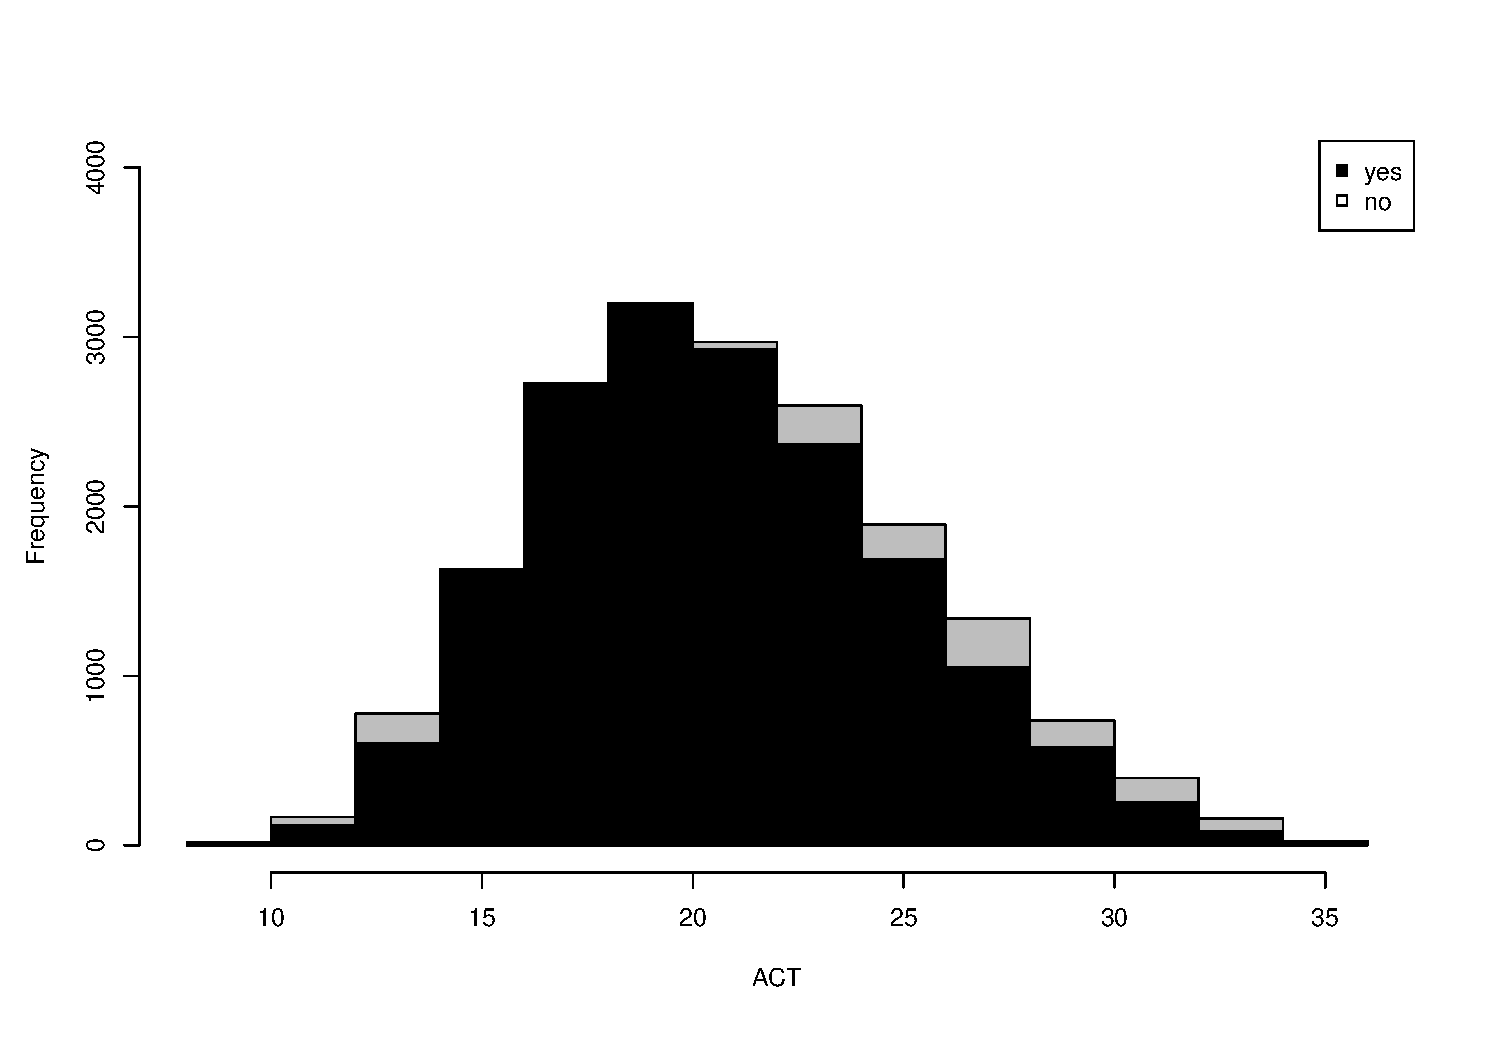
\includegraphics[width=6in, height=2.5in] {pic/enroll_act} %width=\linewidth,
\caption{Histogram for ACT} \label{enroll_act}
\end{figure}

\begin{figure} [H]
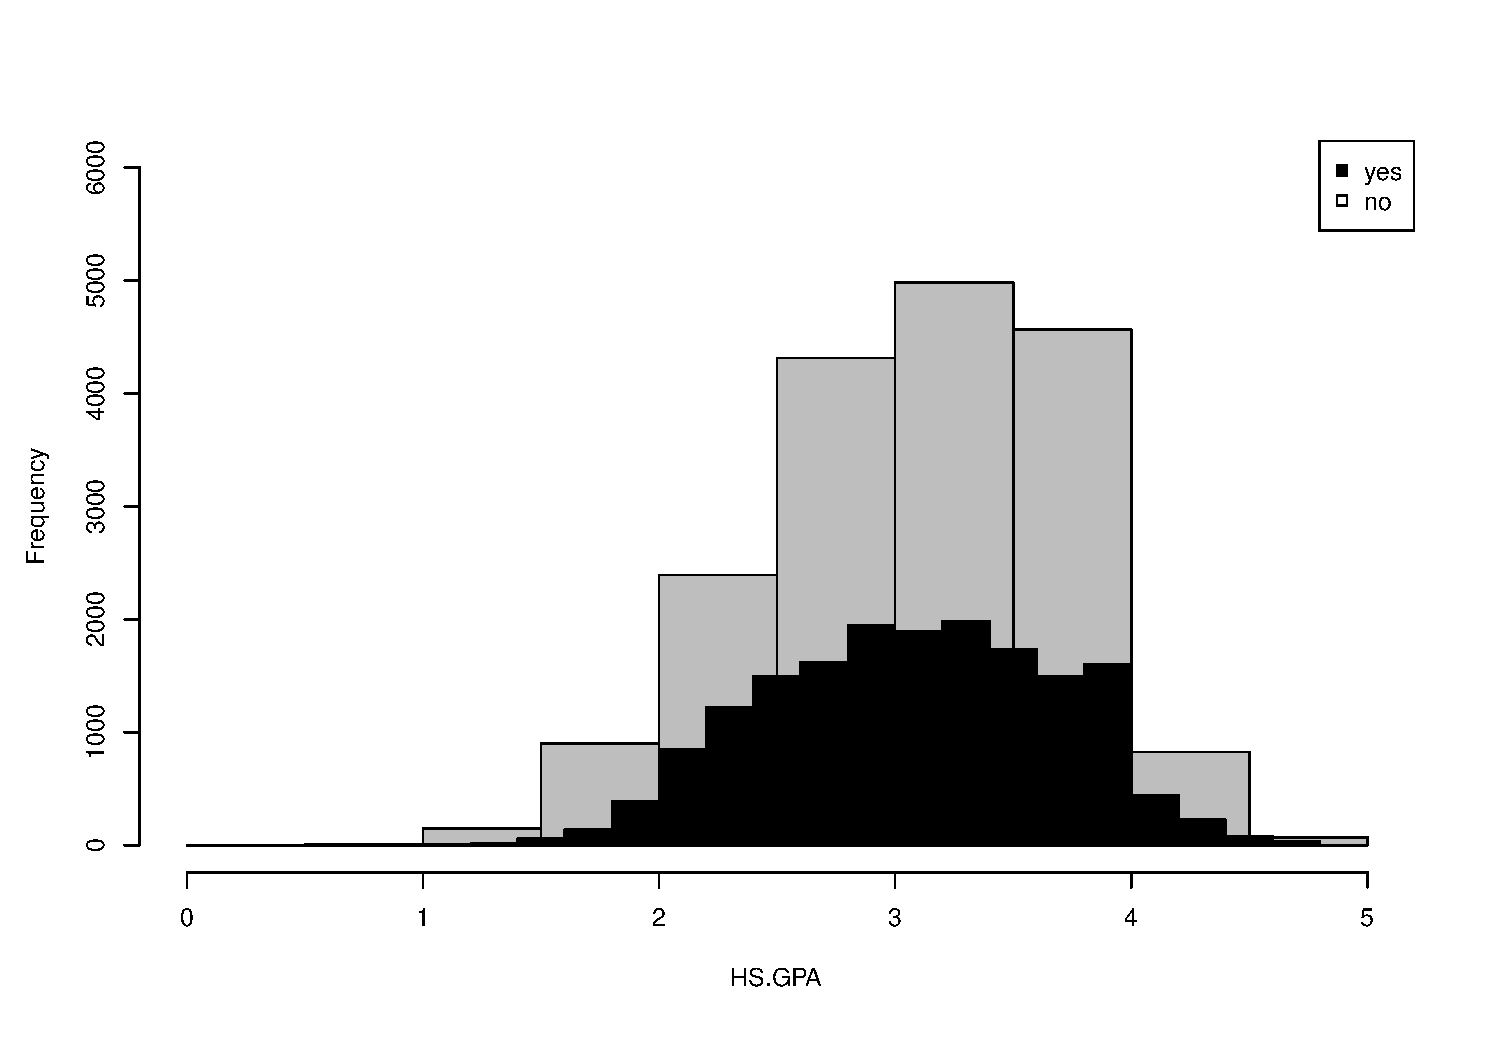
\includegraphics[width=6in, height=2.5in]{pic/enroll_gpa}
\caption{Histogram for High School GPA  } \label{enroll_gpa}
\end{figure}


The characteristics of matriculated students, such as GPA, ACT, etc, as can be seen, are similar to that of the applications.  This is mainly because of the  university's open admission policies and only a minor portion of incomplete applications are being filtered out.  

% \begin{figure}[ht] 

% %\begin{subfigure}{0.48\textwidth}
% %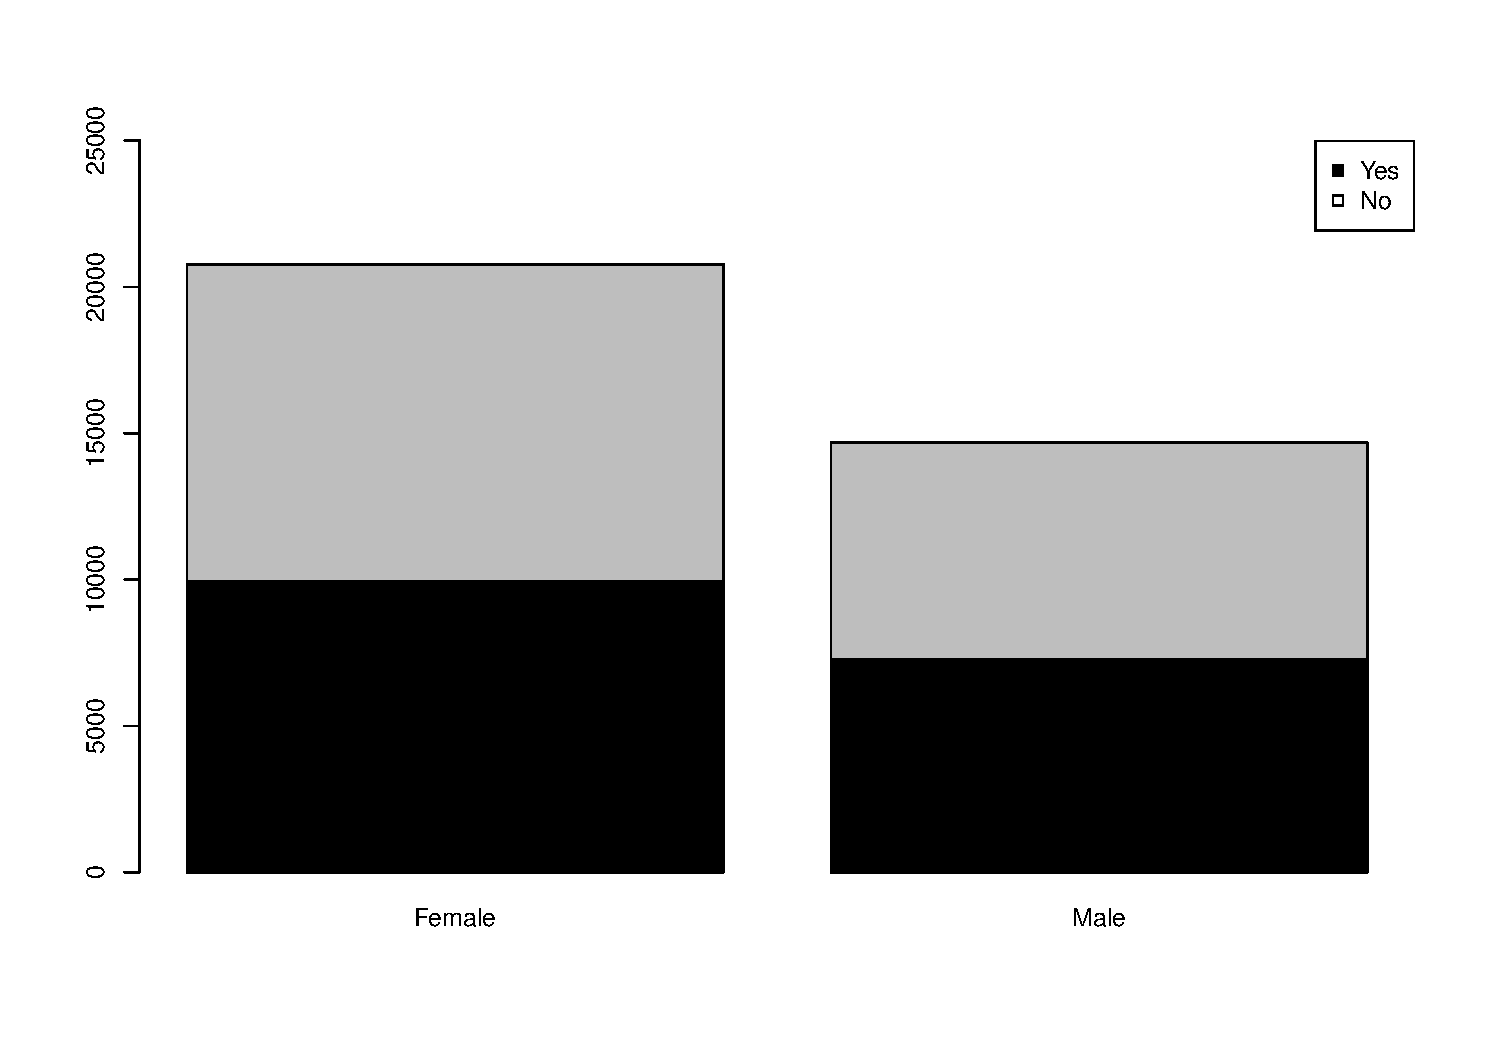
\includegraphics[width=\linewidth]{pic/enroll_gender}
% %\caption{} \label{enroll:a}
% %\end{subfigure}\hspace*{\fill}
% %\begin{subfigure}{0.48\textwidth }
% %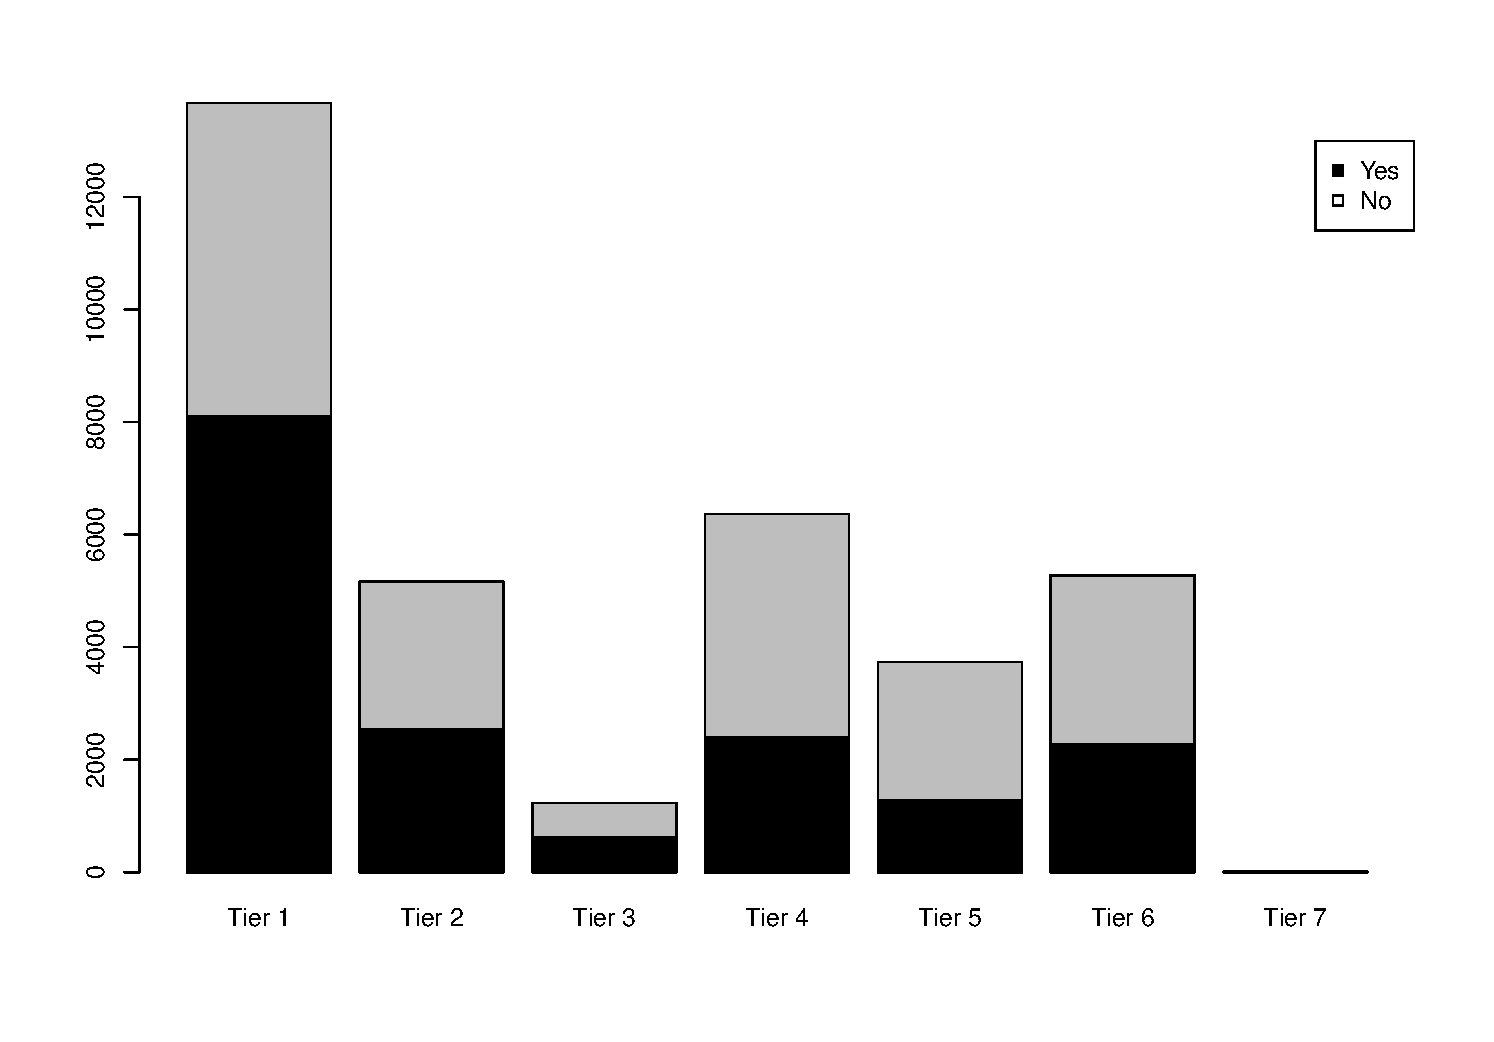
\includegraphics[width=\linewidth]{pic/enroll_tier}
% %\caption{} \label{enroll:b}
% %\end{subfigure}
% %\medskip
% \begin{subfigure}{0.48\textwidth}
% 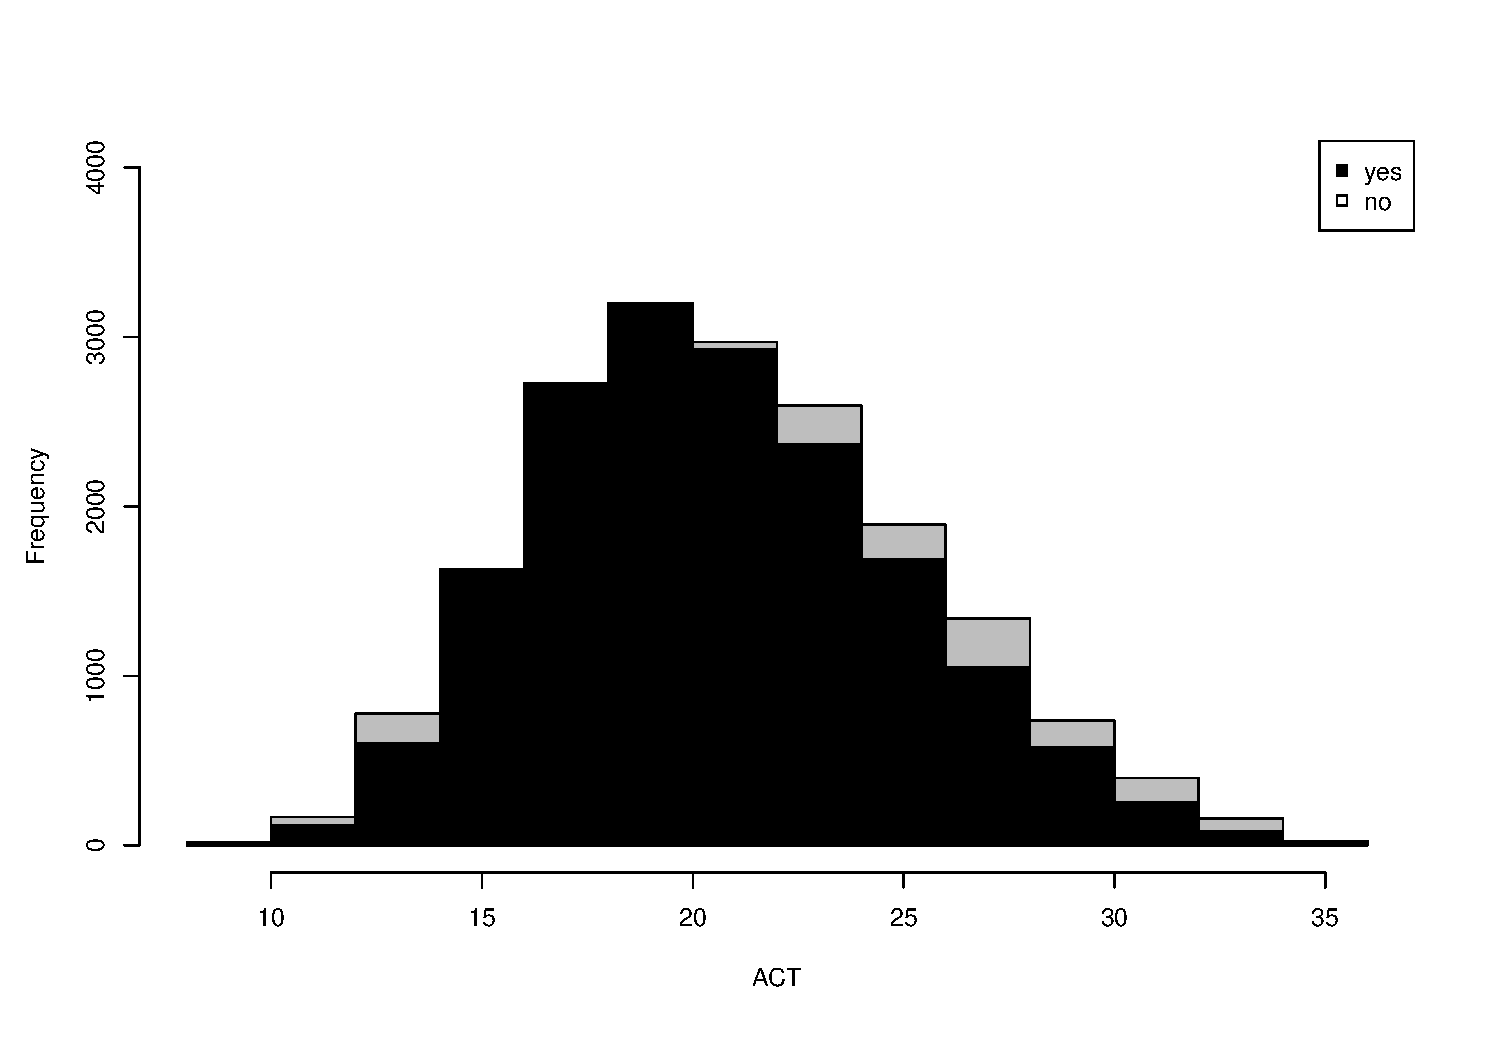
\includegraphics[width=\linewidth] {pic/enroll_act}
% \caption{} \label{enroll:c}
% \end{subfigure}\hspace*{\fill}
% \begin{subfigure}{0.48\textwidth}
% 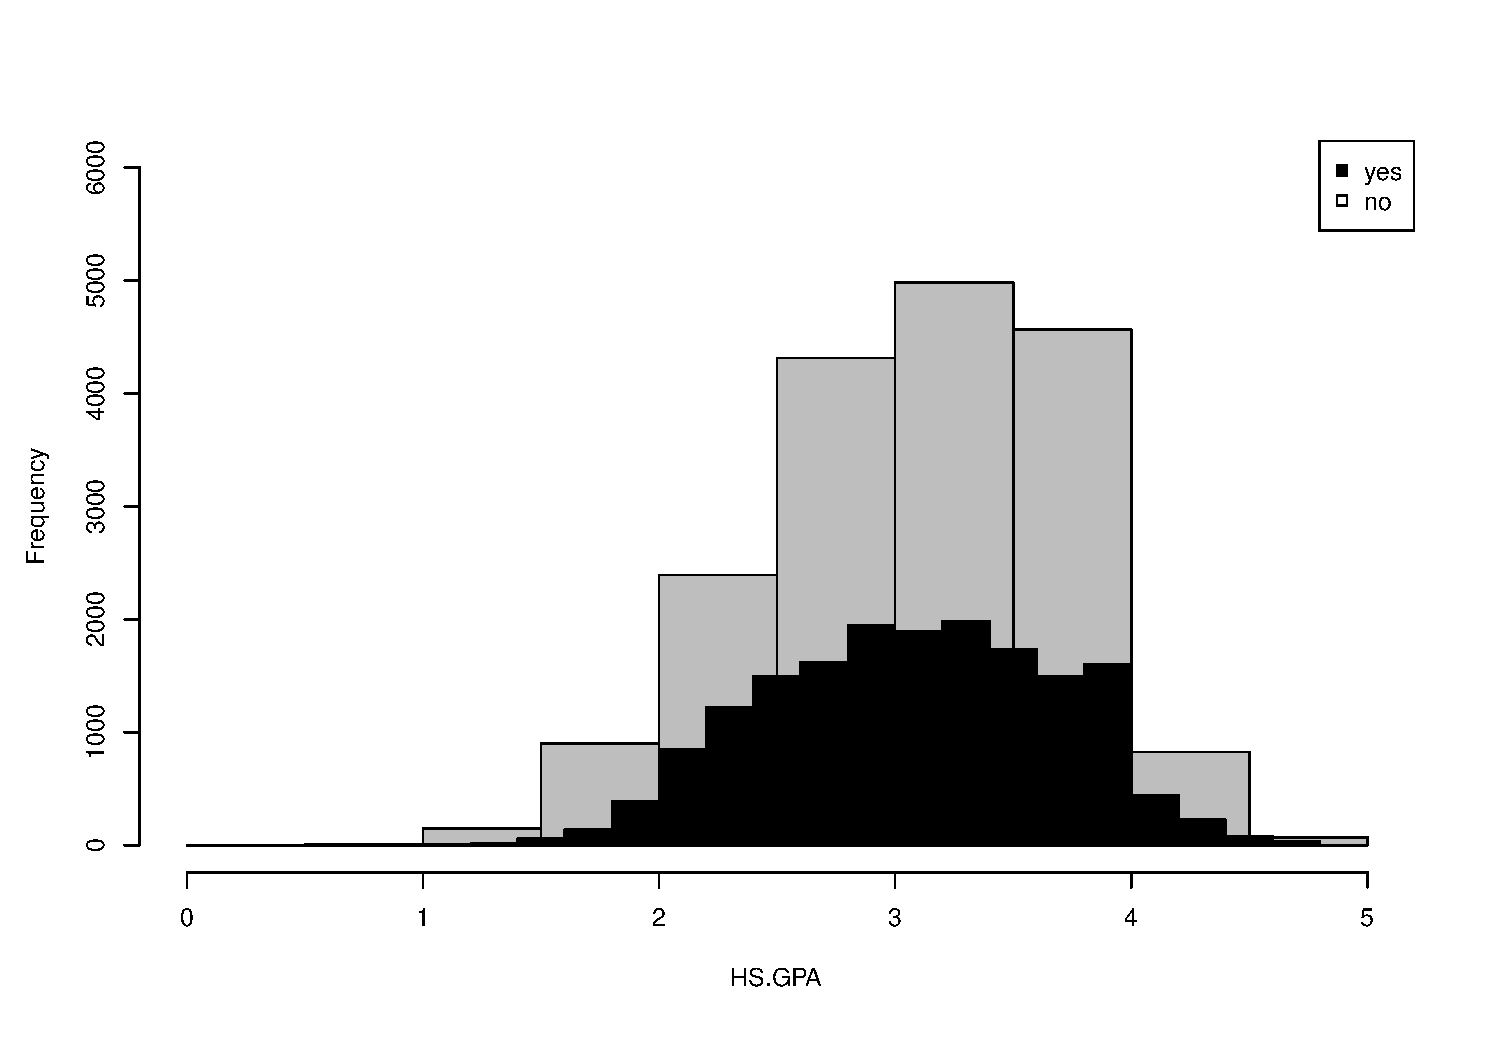
\includegraphics[width=\linewidth]{pic/enroll_gpa}
% \caption{} \label{enroll:d}
% \end{subfigure}

% %\medskip
% %\begin{subfigure}{0.45\textwidth}
% %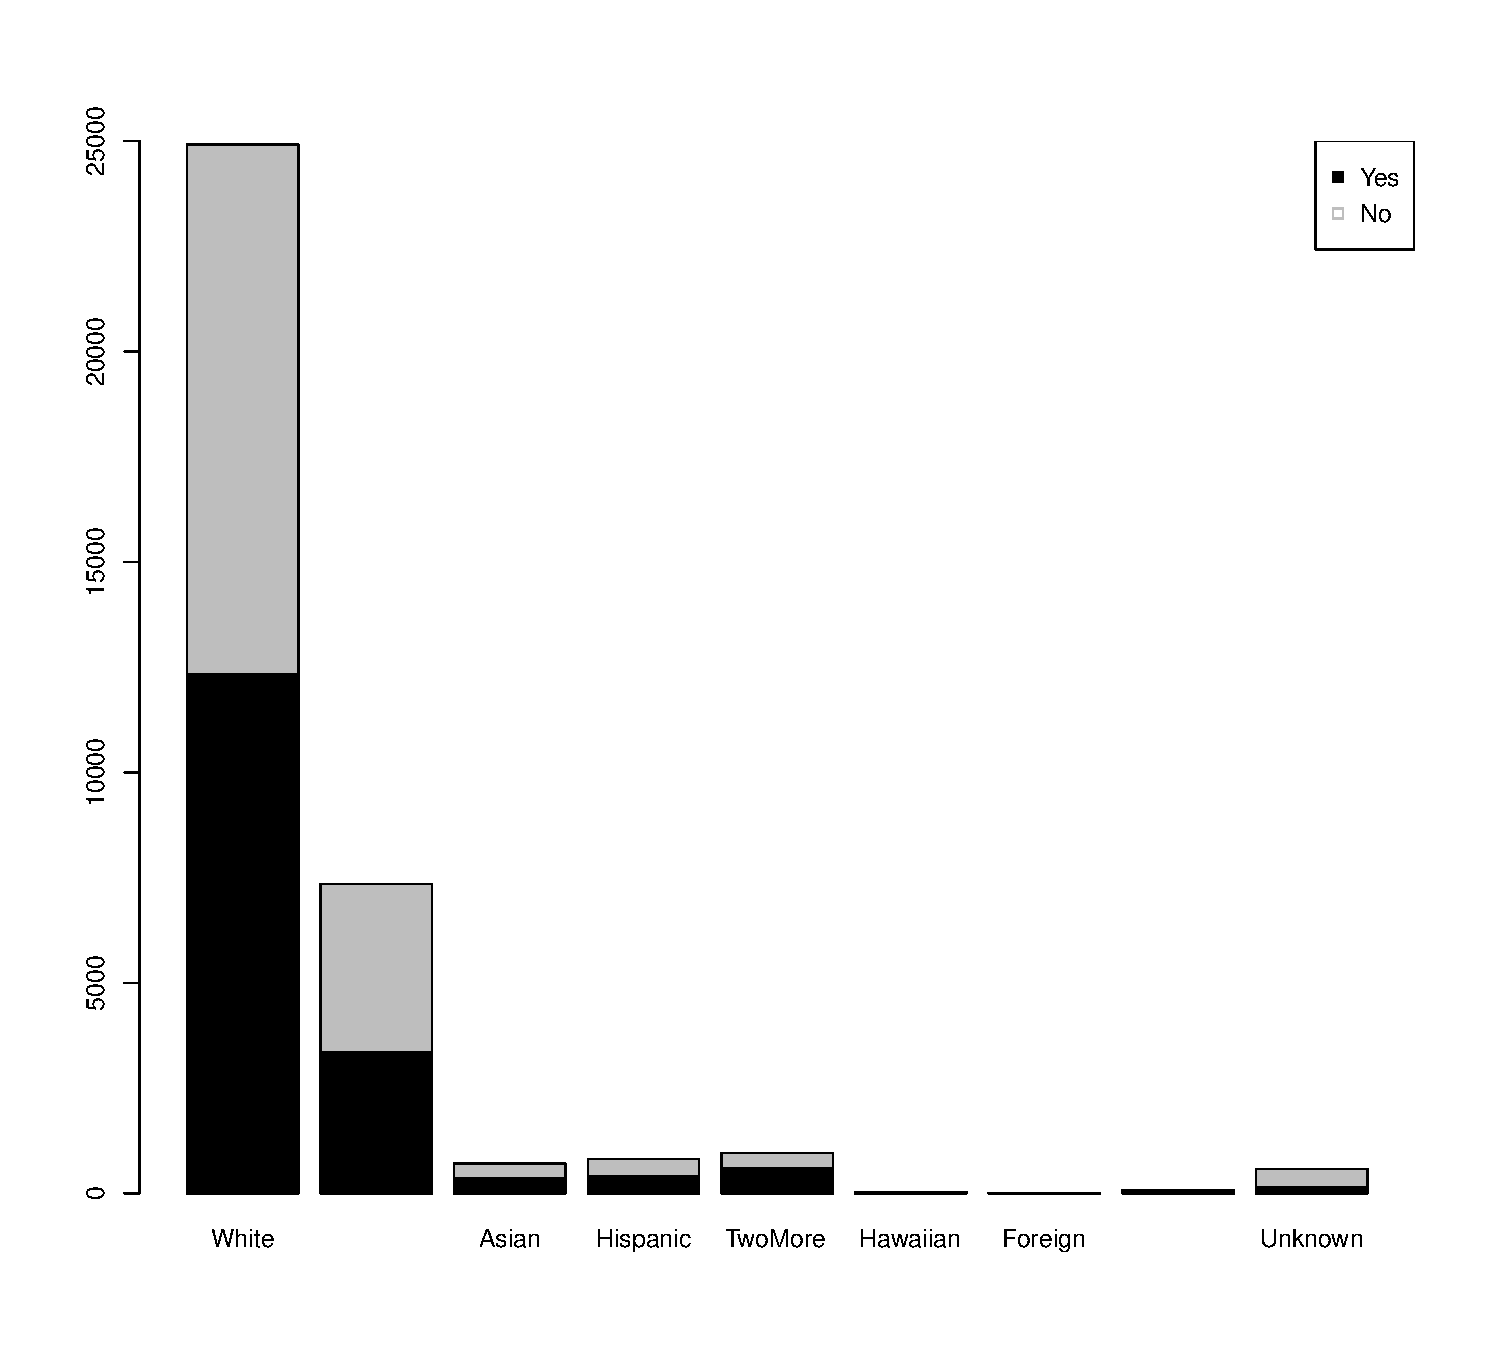
\includegraphics[width=\linewidth, height=6cm]{pic/enroll_ethnicity}
% %\caption{} \label{enroll:e}
% %\end{subfigure}\hspace*{\fill}
% %\begin{subfigure}{0.45\textwidth}
% %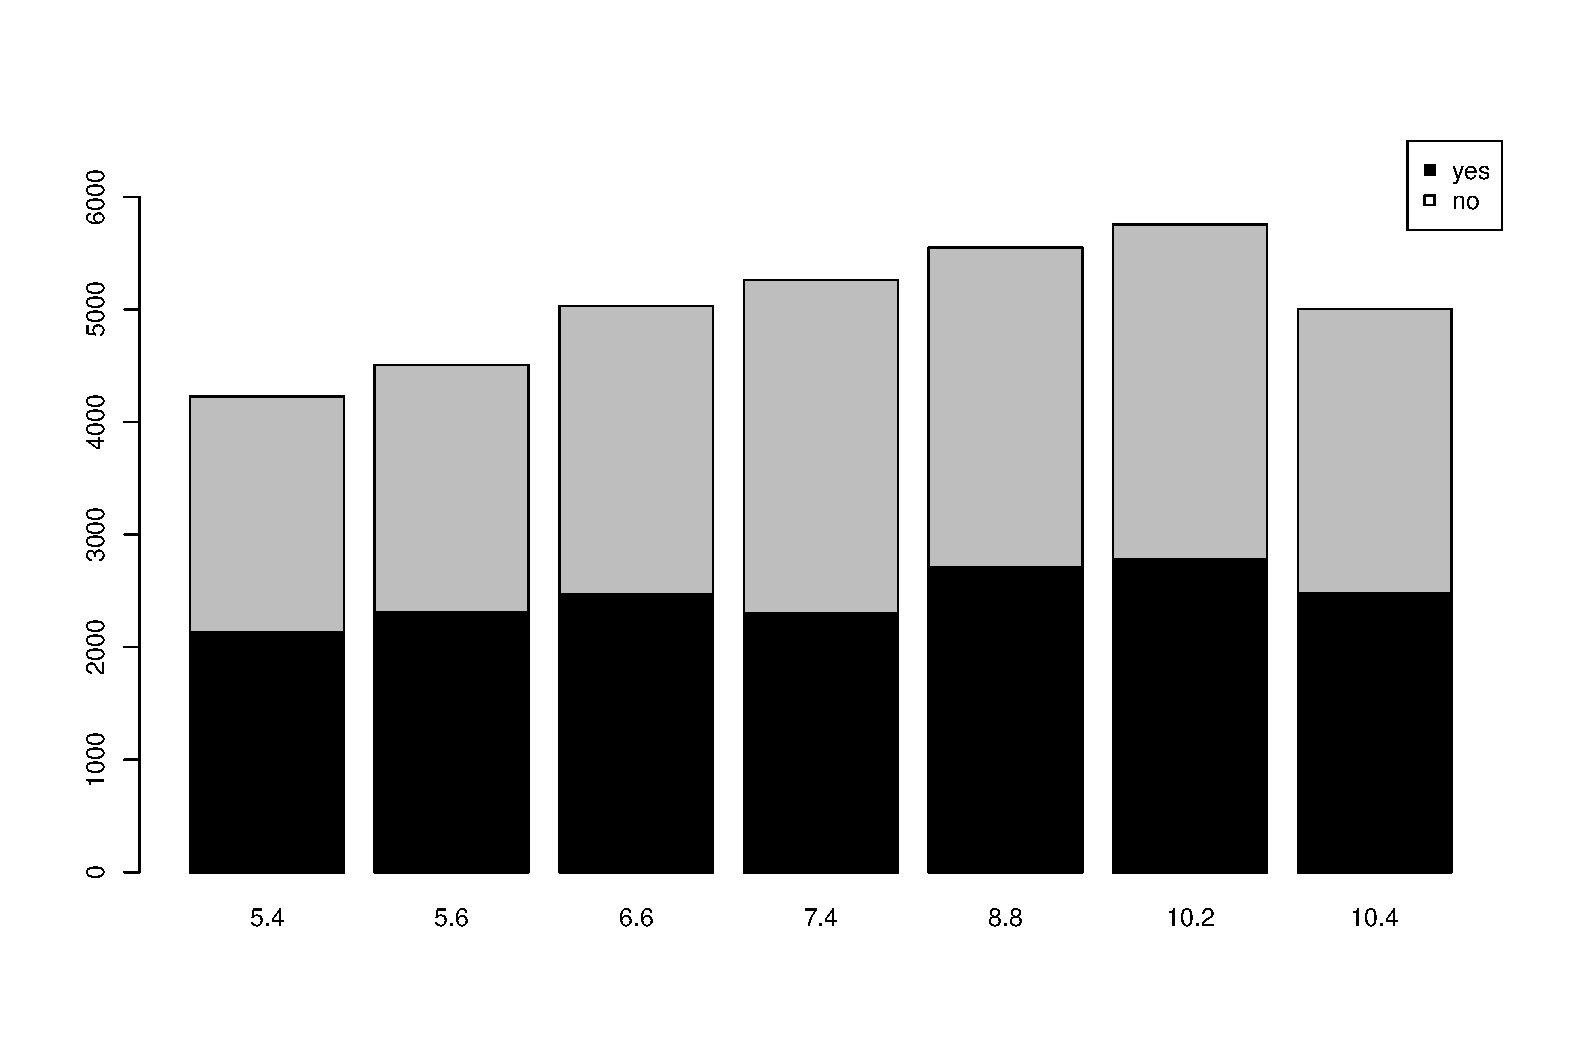
\includegraphics[width=\linewidth, height=6cm]{pic/enroll_index}
% %\caption{} \label{enroll:f}
% %\end{subfigure}
%   \caption{Histogram for some important variables in enrollment prediction: 
%                        (a)  ACT Score (b) High school GPA}
%   \label{enroll_sum} 
% \end{figure}

\vspace{0.1in}
\noindent \textbf{Applicants Across Academic Measures.}  Table \ref{num_act_gpa} shows the number of applicants with specific GPA and ACT scores.  Here the number in the table represents the number of applications with the corresponding GPA (row) and ACT (column) scores. There seems to be a apparent correlation between GPA and ACT that will be discussed later. 

\begin{sidewaystable}[!htbp]
 \resizebox{\linewidth}{200pt}{
\begin{tabular}{@{\extracolsep{5pt}}|c|ccccccccccccccccccccccccccc|c|}
\hline
GPA/ACT     & \multicolumn{1}{c|}{9} & \multicolumn{1}{c|}{10} &
\multicolumn{1}{c|}{11} & \multicolumn{1}{c|}{12} & \multicolumn{1}{c|}{13} &
\multicolumn{1}{c|}{14}  & \multicolumn{1}{c|}{15}  & \multicolumn{1}{c|}{16}
& \multicolumn{1}{c|}{17}  & \multicolumn{1}{c|}{18}  & \multicolumn{1}{c|}{19}
& \multicolumn{1}{c|}{20}  & \multicolumn{1}{c|}{21}  & \multicolumn{1}{c|}{22}
& \multicolumn{1}{c|}{23}  & \multicolumn{1}{c|}{24}  & \multicolumn{1}{c|}{25}
& \multicolumn{1}{c|}{26}  & \multicolumn{1}{c|}{27}  & \multicolumn{1}{c|}{28}
& \multicolumn{1}{c|}{29}  & \multicolumn{1}{c|}{30} & \multicolumn{1}{c|}{31}
& \multicolumn{1}{c|}{32} & \multicolumn{1}{c|}{33} & \multicolumn{1}{c|}{34} &
35 & Grand Total \\ \hline
1           &                        &                         &
&                         & 1                       &
& 2                        &                          &
&                          &                          &
&                          &                          &
&                          &                          &
&                          &                          &
&                         &                         &                         &
&                         &    & 3           \\ \cline{1-1} \cline{29-29}
1.1         &                        &                         &
&                         &                         &
&                          &                          & 1
&                          &                          &
&                          &                          &
&                          &                          &
&                          &                          &
&                         &                         &                         &
&                         &    & 1           \\ \cline{1-1} \cline{29-29}
1.2         &                        &                         &
&                         & 1                       &
&                          &                          &
&                          & 1                        &
&                          &                          &
&                          &                          &
&                          &                          &
&                         &                         &                         &
&                         &    & 2           \\ \cline{1-1} \cline{29-29}
1.3         &                        &                         &
& 1                       &                         &
&                          & 1                        &
& 1                        &                          &
&                          &                          &
&                          &                          &
&                          &                          &
&                         &                         &                         &
&                         &    & 3           \\ \cline{1-1} \cline{29-29}
1.4         &                        &                         &
& 1                       &                         & 2
&                          & 1                        &
&                          & 2                        &
&                          &                          &
&                          &                          &
&                          &                          &
&                         &                         &                         &
&                         &    & 6           \\ \cline{1-1} \cline{29-29}
1.5         &                        &                         &
& 1                       & 2                       & 2
& 1                        & 6                        & 3
&                          & 3                        &
&                          &                          &
&                          &                          & 1
&                          &                          &
&                         &                         &                         &
&                         &    & 19          \\ \cline{1-1} \cline{29-29}
1.6         &                        &                         &
& 1                       & 4                       & 4
& 2                        & 4                        & 4
& 4                        & 2                        & 3
& 2                        & 2                        & 1
& 1                        &                          &
&                          &                          &
&                         &                         &                         &
&                         &    & 34          \\ \cline{1-1} \cline{29-29}
1.7         & 1                      &                         &
& 2                       & 5                       & 4
& 7                        & 3                        & 2
& 5                        & 6                        & 1
& 1                        & 2                        & 1
& 2                        & 2                        & 1
&                          &                          &
&                         &                         &                         &
&                         &    & 45          \\ \cline{1-1} \cline{29-29}
1.8         &                        &                         &
&                         & 4                       & 8
& 5                        & 9                        & 4
& 8                        & 4                        & 1
& 1                        & 1                        &
&                          &                          &
&                          &                          &
&                         &                         &                         &
&                         &    & 45          \\ \cline{1-1} \cline{29-29}
1.9         &                        & 1                       & 1
& 2                       & 1                       & 11
& 9                        & 7                        & 9
& 5                        & 5                        & 5
& 4                        & 3                        & 3
&                          & 2                        &
&                          &                          &
&                         &                         &                         &
&                         &    & 68          \\ \cline{1-1} \cline{29-29}
2           &                        &                         &
& 2                       & 4                       & 5
& 7                        & 14                       & 9
& 10                       & 7                        & 7
& 4                        & 6                        & 3
& 1                        & 1                        &
&                          &                          & 1
&                         &                         &                         &
&                         &    & 81          \\ \cline{1-1} \cline{29-29}
2.1         & 1                      &                         &
& 5                       & 8                       & 7
& 17                       & 23                       & 8
& 14                       & 12                       & 7
& 5                        & 5                        & 2
&                          & 1                        & 1
& 1                        &                          &
& 1                       &                         &                         &
&                         &    & 118         \\ \cline{1-1} \cline{29-29}
2.2         &                        &                         & 1
& 3                       & 7                       & 7
& 11                       & 12                       & 23
& 18                       & 13                       & 13
& 8                        & 5                        & 2
& 7                        & 2                        & 2
& 1                        & 1                        & 1
&                         &                         &                         &
&                         &    & 137         \\ \cline{1-1} \cline{29-29}
2.3         &                        &                         & 1
& 3                       & 5                       & 9
& 21                       & 21                       & 29
& 19                       & 17                       & 15
& 13                       & 5                        & 5
& 7                        & 2                        & 3
& 1                        & 2                        &
&                         &                         &                         &
&                         &    & 178         \\ \cline{1-1} \cline{29-29}
2.4         &                        &                         &
& 1                       & 4                       & 13
& 20                       & 17                       & 30
& 15                       & 16                       & 19
& 21                       & 7                        & 8
& 5                        & 2                        & 3
& 2                        &                          &
& 1                       &                         &                         &
&                         &    & 184         \\ \cline{1-1} \cline{29-29}
2.5         &                        &                         &
& 4                       & 3                       & 13
& 17                       & 26                       & 26
& 22                       & 29                       & 17
& 18                       & 11                       & 7
& 8                        & 3                        & 3
& 1                        & 1                        & 2
&                         & 1                       &                         &
&                         &    & 212         \\ \cline{1-1} \cline{29-29}
2.6         &                        &                         & 1
& 3                       & 4                       & 10
& 10                       & 21                       & 26
& 38                       & 28                       & 15
& 13                       & 5                        & 13
& 11                       & 5                        & 2
& 4                        &                          & 2
& 1                       &                         &                         &
1                       &                         &    & 213         \\
\cline{1-1} \cline{29-29}
2.7         &                        &                         & 3
&                         & 2                       & 7
& 17                       & 22                       & 32
& 27                       & 33                       & 23
& 15                       & 15                       & 15
& 7                        & 3                        & 2
& 1                        & 1                        &
& 2                       &                         &                         &
&                         &    & 227         \\ \cline{1-1} \cline{29-29}
2.8         &                        &                         &
& 2                       & 4                       & 7
& 12                       & 10                       & 28
& 27                       & 29                       & 23
& 19                       & 20                       & 14
& 13                       & 4                        & 7
& 5                        & 2                        & 1
&                         &                         &                         &
1                       &                         &    & 228         \\
\cline{1-1} \cline{29-29}
2.9         &                        &                         & 1
& 2                       & 7                       & 9
& 11                       & 25                       & 21
& 39                       & 32                       & 40
& 20                       & 22                       & 20
& 15                       & 12                       & 11
& 4                        & 1                        &
&                         &                         &                         &
&                         &    & 292         \\ \cline{1-1} \cline{29-29}
3           &                        &                         &
& 1                       & 1                       & 9
& 9                        & 16                       & 26
& 34                       & 33                       & 35
& 28                       & 28                       & 26
& 17                       & 15                       & 10
& 3                        & 2                        & 5
&                         & 2                       &                         &
& 1                       &    & 301         \\ \cline{1-1} \cline{29-29}
3.1         &                        &                         &
& 3                       & 2                       & 6
& 12                       & 11                       & 18
& 36                       & 35                       & 39
& 38                       & 18                       & 24
& 21                       & 15                       & 11
& 4                        & 4                        & 2
& 1                       &                         &                         &
&                         & 1  & 301         \\ \cline{1-1} \cline{29-29}
3.2         &                        &                         &
&                         &                         & 6
& 7                        & 17                       & 19
& 26                       & 26                       & 32
& 29                       & 37                       & 32
& 16                       & 16                       & 8
& 12                       & 3                        & 8
& 5                       & 4                       & 1                       &
&                         &    & 304         \\ \cline{1-1} \cline{29-29}
3.3         &                        &                         & 1
&                         & 1                       & 4
& 8                        & 5                        & 23
& 22                       & 31                       & 33
& 22                       & 34                       & 27
& 22                       & 27                       & 19
& 13                       & 10                       & 4
& 3                       & 5                       &                         &
1                       & 2                       &    & 317         \\
\cline{1-1} \cline{29-29}
3.4         &                        & 1                       &
&                         & 1                       &
& 3                        & 9                        & 9
& 14                       & 21                       & 31
& 36                       & 35                       & 30
& 26                       & 21                       & 16
& 10                       & 8                        & 5
& 2                       & 3                       &                         &
&                         &    & 281         \\ \cline{1-1} \cline{29-29}
3.5         &                        &                         &
&                         &                         &
& 5                        & 5                        & 8
& 13                       & 16                       & 23
& 27                       & 29                       & 25
& 29                       & 30                       & 22
& 14                       & 11                       & 5
& 7                       & 2                       &                         &
1                       &                         &    & 272         \\
\cline{1-1} \cline{29-29}
3.6         &                        &                         &
&                         &                         &
& 2                        & 3                        & 4
& 3                        & 22                       & 17
& 21                       & 30                       & 37
& 28                       & 23                       & 25
& 18                       & 11                       & 10
& 6                       & 1                       & 3                       &
2                       & 2                       &    & 268         \\
\cline{1-1} \cline{29-29}
3.7         &                        &                         &
&                         &                         & 2
& 1                        &                          & 3
& 7                        & 12                       & 10
& 20                       & 20                       & 28
& 28                       & 22                       & 25
& 23                       & 16                       & 13
& 5                       & 2                       & 2                       &
& 2                       &    & 241         \\ \cline{1-1} \cline{29-29}
3.8         &                        &                         &
&                         &                         &
& 2                        &                          &
& 3                        & 8                        & 13
& 13                       & 20                       & 18
& 29                       & 19                       & 18
& 27                       & 15                       & 11
& 10                      & 3                       & 2                       &
2                       &                         &    & 213         \\
\cline{1-1} \cline{29-29}
3.9         &                        &                         &
&                         &                         &
& 1                        & 2                        & 2
& 3                        & 6                        & 6
& 8                        & 14                       & 24
& 26                       & 19                       & 25
& 19                       & 17                       & 18
& 11                      & 7                       & 5                       &
3                       & 1                       &    & 217         \\
\cline{1-1} \cline{29-29}
4           &                        &                         &
&                         &                         &
&                          & 1                        &
&                          & 2                        & 7
& 7                        & 7                        & 20
& 18                       & 19                       & 23
& 23                       & 21                       & 20
& 22                      & 9                       & 11                      &
12                      & 7                       & 2  & 231         \\
\cline{1-1} \cline{29-29}
4.1         &                        &                         &
&                         &                         &
&                          &                          & 1
&                          & 2                        & 2
& 1                        & 3                        & 7
& 8                        & 4                        & 6
& 9                        & 4                        & 4
& 6                       & 4                       & 2                       &
3                       & 1                       &    & 67          \\
\cline{1-1} \cline{29-29}
4.2         &                        &                         &
&                         &                         &
&                          &                          &
& 1                        &                          & 1
& 2                        & 4                        & 1
& 3                        & 5                        & 5
& 7                        & 3                        & 4
& 3                       & 2                       & 5                       &
1                       & 1                       &    & 48          \\
\cline{1-1} \cline{29-29}
4.3         &                        &                         &
&                         &                         &
&                          &                          &
&                          &                          &
&                          & 1                        & 2
& 4                        & 3                        & 2
& 2                        & 8                        & 3
& 3                       & 4                       & 4                       &
1                       & 1                       &    & 38          \\
\cline{1-1} \cline{29-29}
4.4         &                        &                         &
&                         &                         &
&                          &                          &
&                          &                          &
&                          &                          &
& 1                        & 4                        & 2
& 3                        & 1                        & 1
& 5                       & 2                       & 2                       &
1                       & 2                       &    & 24          \\
\cline{1-1} \cline{29-29}
4.5         &                        &                         &
&                         &                         &
&                          &                          &
&                          &                          & 1
&                          & 1                        & 4
&                          & 1                        & 1
&                          & 1                        & 3
&                         & 1                       & 2                       &
3                       &                         & 1  & 19          \\
\cline{1-1} \cline{29-29}
4.6         &                        &                         &
&                         &                         &
&                          &                          &
&                          &                          &
&                          &                          & 1
&                          &                          & 1
& 1                        & 1                        &
& 1                       &                         & 3                       &
1                       & 1                       &    & 10          \\
\cline{1-1} \cline{29-29}
4.7         &                        &                         &
&                         &                         &
&                          &                          &
&                          &                          &
& 1                        &                          &
&                          &                          & 1
& 3                        & 1                        &
&                         & 1                       & 1                       &
1                       &                         &    & 9           \\
\cline{1-1} \cline{29-29}
4.8         &                        &                         &
&                         &                         &
&                          &                          &
&                          &                          &
&                          &                          &
&                          &                          &
& 1                        & 1                        &
& 1                       &                         &                         &
&                         &    & 3           \\ \hline
Grand Total & \multicolumn{1}{c|}{2} & \multicolumn{1}{c|}{2}  &
\multicolumn{1}{c|}{9}  & \multicolumn{1}{c|}{37} & \multicolumn{1}{c|}{71} &
\multicolumn{1}{c|}{145} & \multicolumn{1}{c|}{219} & \multicolumn{1}{c|}{291}
& \multicolumn{1}{c|}{368} & \multicolumn{1}{c|}{414} &
\multicolumn{1}{c|}{453} & \multicolumn{1}{c|}{439} & \multicolumn{1}{c|}{397}
& \multicolumn{1}{c|}{390} & \multicolumn{1}{c|}{400} &
\multicolumn{1}{c|}{353} & \multicolumn{1}{c|}{282} & \multicolumn{1}{c|}{256}
& \multicolumn{1}{c|}{212} & \multicolumn{1}{c|}{146} &
\multicolumn{1}{c|}{123} & \multicolumn{1}{c|}{96} & \multicolumn{1}{c|}{53} &
\multicolumn{1}{c|}{43} & \multicolumn{1}{c|}{34} & \multicolumn{1}{c|}{21} & 4
& 5260        \\ \hline
\end{tabular}}
\caption{Number of applicants vs GPA/ACT in 2012-2013}
\label{num_act_gpa}
\end{sidewaystable}


\newpage
\section{Logistic Regression For Enrollment \& Graduation}
\subsection{Logistic Regression Methodology}

%\noindent \textbf{Logistic Regression.} 
Logistic regression is a popular method when predicting variables with dichotomous outcomes (yes and no) such as enroll (yes) and do not enroll (no). The output of a logistic regression model is the probability of the enrollment levels. Specifically, in this research, the probabilities to be sought are:

\noindent \textbf{Enrollment probability:} what is the probability of enrollment (yes) for an applicant with, say, a GPA of 2.5, an ACT of 28, given a \$1,000 scholarship?

\noindent \textbf{Graduation probability:} what is the probability of graduation (yes) for the same applicant?

\vspace{0.15in}
%\noindent \textbfx{Methodology.} 
Let us denote $p^e(x)$ and $p^g(x)$ as the enrollment and graduation probability respectively. Because the probability $p(x)$ must fall in $[0,1]$th, a regular linear regression is unsuitable as the regression function is not bounded. To resolve this issue, a ratio, called the odds of success and defined as  $\frac{p(x)}{1-p(x)}$,  is used to form a regression model and and a logistic function is defined as:
\begin{equation}
\ensuremath{¡=\beta_0+\beta_1 x_1+\beta_2 x_2 +\ldots+\beta_k x_k}
¡\end{equation}
The probability of enrollment or graduation can thus be rewritten as:
\begin{equation}
p(x)=\frac{e^{\beta_0+\beta_1 x_1+\beta_2 x_2 +\ldots+\beta_i x_i}}{1+e^{\beta_0+\beta_1 x_1+\beta_2 x_2 +\ldots+\beta_ix_i}}
=\frac{1}{1+e^{-(\beta_0+\beta_0+\beta_1 x_1+\beta_2 x_2 +\ldots+\beta_k x_k)}}
\end{equation}
Here, $\beta_0$ is the intercept and $\beta_1 \ldots \beta_i$ are parameters for corresponding variable $x_i$.  Here $x_i$ could be either continuous
variables such as GPA or  ACT, or categorical variables such as gender, ethnicity, or region.  Parameters $\beta_0$ and $\beta_i$ are estimated by the maximum likelihood estimation.
\begin{equation}
\ell(\beta_0,\ldots \beta_i) = \prod_{i:y_i=1} p(x_i)
\prod_{i^{'}:y_i{^{'}=0}} (1-p(x_{i^{'}}))
\end{equation}
For details on the derivation of the parameter estimations, please see \citet{Hosmer2013}.

\begin{comment}
This function will always generate an S-shape curve as shown below:
\begin{figure}[ht]
   \centering
 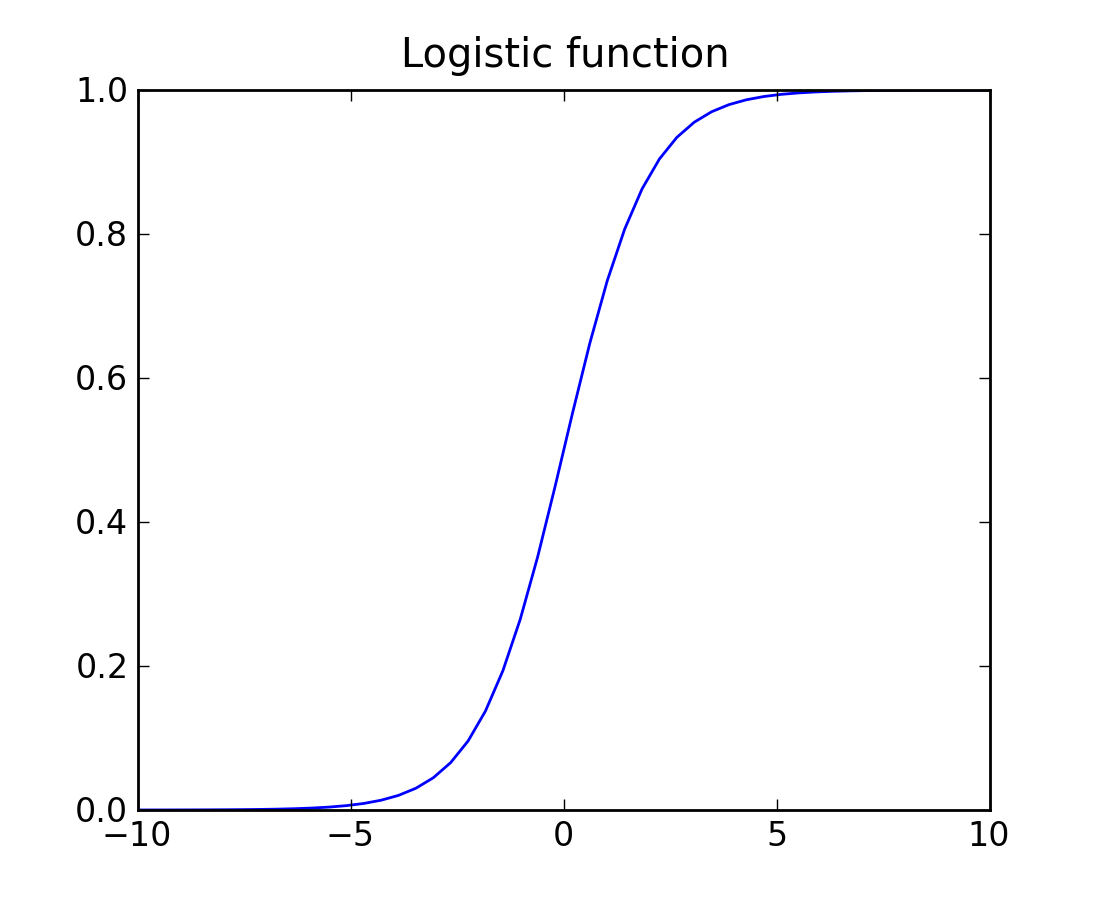
\includegraphics[scale=0.5]{pic/LR_EXAMPLE}
 \caption{Logistic Regression Example}
\end{figure}
\end{comment}

\begin{comment}
\textbf{An example of a cumulative distribution function plot of logistic
regression is shown below, which has a "S" shaped curves between 0 and 1.}
\begin{figure}[h!]
   \centering
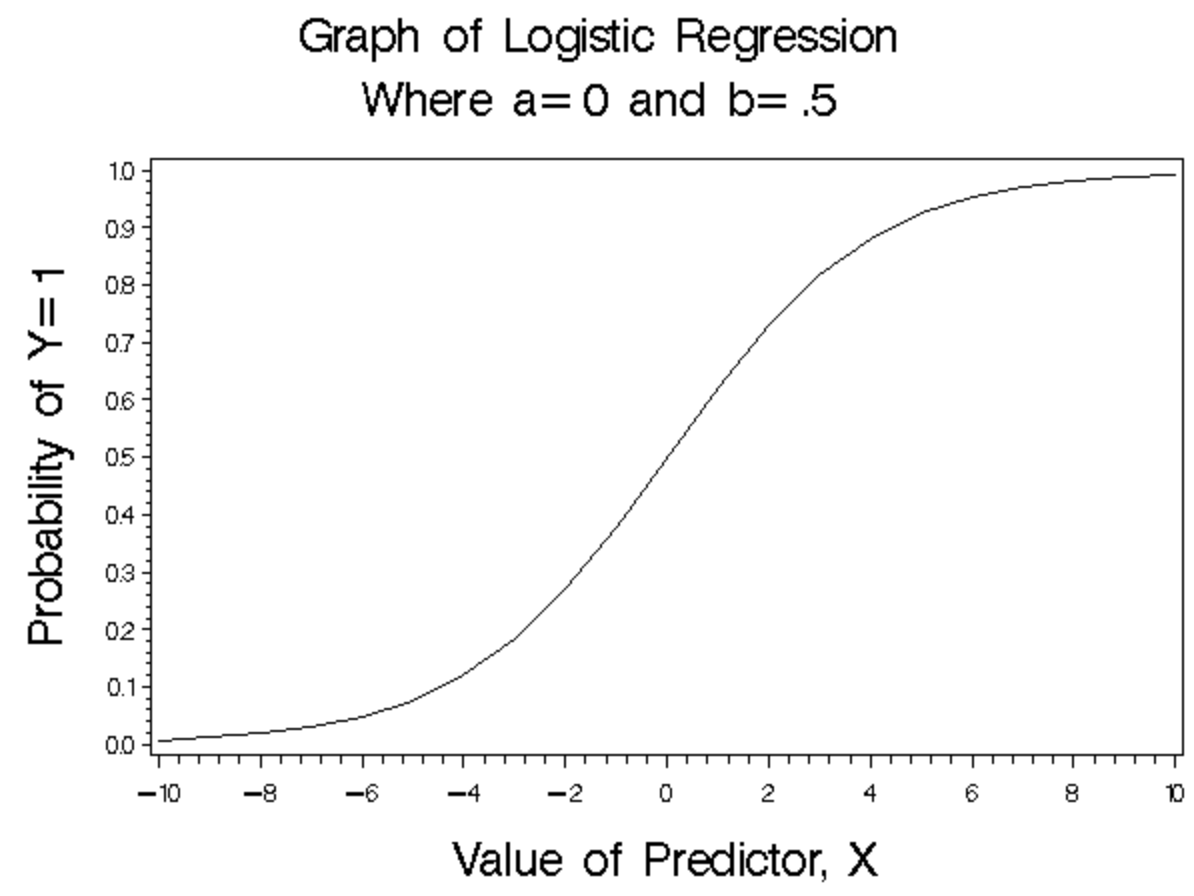
\includegraphics[width=0.4\textwidth]{LR.png}
 \caption{"S" shaped curve in logistic regression}
\end{figure}
\end{comment}

\subsection{Collinearity and Variable Selection}
The baseline model is a general linear logistic regression model.  Before the model is presented, collinearity among variables and variable selections are  first explored.

\vspace{0.15in}
\noindent \textbf{Collinearity. } Collinearity refers to the fact that two or more predictor variables within the regression models are highly correlated.  Collinearity makes the estimate highly unstable, i.e., coefficient estimates are very sensitive to small changes due  the model or data. As a result,  it is hard to interpret which variables are contributing to the model and to identify how exactly each variable is contributing to the model \citep{belsley2005regression, Midi2010}. For this study, the correlation matrix, a common method to examine collinearity,  of selected continuous variables is presented in Table \ref{correlation_matrix}. 

%\begin{sidewaystable}[!htbp]
\begin{table}[H]
\begin{tabular}{@{\extracolsep{4pt}} |l|ccccc|} \hline  %\hline 
& GPA            & ACT    & \begin{tabular}[c]{@{}c@{}}HS.\\
PERCENTILE\end{tabular} & \begin{tabular}[c]{@{}c@{}}SCHOLAR-\\
SHIP\end{tabular} & \begin{tabular}[c]{@{}c@{}} 
PELL.\\ GRANT\end{tabular}
\\ \hline %\hline     
GPA         & 1       & 0.596  & \textbf{0.884} & 0.612                 & -0.190  \\
ACT                & 0.596          & 1      & 0.469 & 0.586            & -0.275 \\
HS.PERCENTILE      & \textbf{0.884} & 0.469  & 1 & 0.594 & -0.060 \\
SCHOLARSHIP        & 0.612          & 0.586  & 0.594   & 1 & 0.025 \\
PELL.GRANT         & -0.190         & -0.275 & -0.060  & 0.025 & 1 \\
\hline                                                             
\end{tabular}
\caption{Pearson correlation matrix of all numeric variables} 
\label{correlation_matrix} 
\end{table}

As can be seen from Table \ref{correlation_matrix},  according to \citep{hinkle2003applied}, there exists a) a high correlation between GPA and HS.PERCENTILE, b) a high correction between academic performance measures such as GPA and ACT, c) a high correlation between scholarship and academic performance measures such as GPA and ACT,  and d) a negative correlation between Pell Grant and academic performance (such as GPA and ACT). Though some of the correlations may not be surprising, the last one seems to suggest that  family income could impact a student's academic performance.  

Collinearity does not reduce the predictive power or reliability of the model as a whole, but it does affect calculations regarding individual predictors and
may not give valid results about any individual predictor, or about which predictors are redundant with respect to others.

\vspace{0.15in}
\noindent \textbf{Variable Selection. }  In regression analysis with multiple variables, strategies have been designed to select the best variables in the model. Stepwise selection is one of the most popular procedures and is adopted in this study \citep{konishi2008information}.

The stepwise variable selection includes backward elimination, forward selection, and bidirectional elimination. A backward stepwise regression, for example, works as follows: a) start with the model containing all potential predictors; b) try subtracting one predictor at a time, keeping the predictor out if doing so improves the measure of predictive accuracy; and c) iterate until no further improvement. 


To determine the best models in the process, several criteria have been proposed, and for logistic regression, the most common ones are BIC, AIC, and AICc. In this paper, the AIC is adopted due to its popularity.  There is always a trade-off between model simplicity and accuracy, and the AIC methods determine whether additional variables are justified. For details, please see \citep{wagenmakers2004aic}
     
In an enrollment model, say with n predictor variables, to get the optimal model, a brute-force approach would have to evaluate $2^{n}$ possible models. The stepwise variable selection evaluates only a limited number of models and presents a heuristic solution to the problem in a fraction of the time.  


\begin{comment}

%%%%%%%%%%%%%%%%%%%%%%%%%%%%%%%%%  BACKWARD SELECTION PROCEDURE

%The detailed backward stepwise selection process is shown in Table \ref{back}.  In the table, the ``step" column represents the number of iterations; the ``model" column represents the model in each iteration; the ``AIC" column represents the AIC value.  As can be seen, the process started with a full model with all of the predictor variables and continued to seek models with lower AIC.  The model ends up only included variables: GPA, ACT, HS.PERCENTILE, APP.COLLEGE, DISTANCE.BIN, HS.COUNTY.TIER, GENDER, PELL.GRANT, ETHNICITY.

\begin{table}[]
%\begin{sidewaystable*}
\centering
\caption{Backward stepwise model selection for enrollment model}
\label{back}
\begin{adjustbox}{width=1.0\textwidth} 
\begin{tabular}{clll}
\hline
Step & Model                                                                   
& Variable Dropped                                        &
\multicolumn{1}{c}{AIC} \\ \hline
1    & \begin{tabular}[c]{@{}l@{}}MATRICULATION $\sim$ GPA + ACT +
HS.PERCENTILE + comb + APP.COLLEGE +,DISTANCE.NUM\\  + DISTANCE.BIN +
HS.COUNTY.TIER + HS.RAIDER.COUNTRY + GENDER + PELL.GRANT + \\ ETHNICITY +
UNDERREPRESENTED + UNEMPLOYMENT.INDEX +SCHOLARSHIP\_PER\end{tabular} &         
& 46262                   \\
2    & \begin{tabular}[c]{@{}l@{}}MATRICULATION $\sim$ GPA + ACT +
HS.PERCENTILE + APP.COLLEGE + DISTANCE.NUM \\ +DISTANCE.BIN + HS.COUNTY.TIER +
HS.RAIDER.COUNTRY + GENDER + PELL.GRANT + \\ ETHNICITY + UNDERREPRESENTED +
UNEMPLOYMENT.INDEX +SCHOLARSHIP\_PER\end{tabular}       & comb                 
& 46262                   \\
3    & \begin{tabular}[c]{@{}l@{}}MATRICULATION $\sim$ GPA + ACT +
HS.PERCENTILE + APP.COLLEGE + DISTANCE.NUM \\ +DISTANCE.BIN + HS.COUNTY.TIER +
HS.RAIDER.COUNTRY + GENDER + PELL.GRANT + \\ ETHNICITY + UNEMPLOYMENT.INDEX +
SCHOLARSHIP\_PER\end{tabular}                         & comb, UNDERREPRESENTED 
& 46260                   \\
4    & \begin{tabular}[c]{@{}l@{}}MATRICULATION $\sim$ GPA + ACT +
HS.PERCENTILE + APP.COLLEGE + DISTANCE.NUM + \\ DISTANCE.BIN + HS.COUNTY.TIER +
GENDER + PELL.GRANT + ETHNICITY \\ +UNEMPLOYMENT.INDEX +
SCHOLARSHIP\_PER\end{tabular}                                             &
comb, UNDERREPRESENTED, HS.RAIDER.COUNTRY               & 46258                
\\
5    & \begin{tabular}[c]{@{}l@{}}MATRICULATION $\sim$ GPA + ACT +
HS.PERCENTILE + APP.COLLEGE + DISTANCE.BIN + \\ HS.COUNTY.TIER + GENDER +
PELL.GRANT + ETHNICITY +\\  UNEMPLOYMENT.INDEX + SCHOLARSHIP\_PER\end{tabular} 
& comb, UNDERREPRESENTED, HS.RAIDER.COUNTRY, DISTANCE.NUM & 46257              
\\
\hline
\end{tabular}
\end{adjustbox}
%\end{sidewaystable*}
\end{table}


\end{comment}

 
\begin{comment}
\paragraph{Goodness of Fit for Logistic Regression Model}
%There are many tests that can be applied to evaluate the effectiveness of a logistic regression model. Of them, four of the commonly used tests are (a)
tests of individual predictors, (b) overall model evaluation, (c) validation of predicted probabilities, (d) goodness of fit statistics. \citet{lr_summary}

Goodness of fit statistics are the most used in the evaluation of logistic regression model \citet{lr_summary} and several methods have been proposed.

The most straightforward method of evaluation  is to calculate the accuracy of the fitted value.  A cut-of value (in percentage) , say 60\%, is chosen and any
predicted value greater than the cut-off will be a successful prediction and any value below will be a failure. This analysis can be entered into a
two-by-two table, called a 'classification table' (or 'confusion matrix') as shown below:
  
% Please add the following required packages to your document preamble:
% \usepackage{multirow}
\begin{table}[h]
\centering
\label{my-label}
\begin{tabular}{|c|c|c|c|}
\hline
     & \multicolumn{3}{c|}{Actual Class}       \\ \hline
\multirow{3}{*}{\begin{tabular}[c]{@{}c@{}}Predicted\\  Class\end{tabular}} &
& Yes   & No    \\ \cline{2-4}
 & Yes & True Positive       & False Positive \\ \cline{2-4} 
& No  & \multicolumn{1}{l|}{False Negative} & True Negative  \\ \hline
\end{tabular}
\caption{Classification Table}
\end{table}

%The limitation of this measurement is that it does not have any measure of significance.This means that 99\% accuracy can be excellent in some cases and
terrible in others. Another limitation is that it assumes equal cost for both error types (false negatives and false positives).

Rather than a single cutoff value, another method of evaluation is  ROC (Receiver Operating Characteristic curve)  which extends the cutoff to all
possible values from 0 to 1. An ROC curve (shown in the Figure \ref{roc_example} below) illustrates the performance of a binary classifier
system as its discrimination threshold is varied.  The curve is created by plotting the true positive rate against the false positive rate at various
threshold settings. Here, the dotted diagonal line is the random prediction. In ROC curve, AUC (area under the curve) indicates the overall quality of the
model. In this case the AUC= 0.9342 which shows an excellent prediction. The closer the ROC curve bulges towards the upper-left corner, the more accurate
the test is.

%The true-positive rate is also known as sensitivity or the sensitivity index d', known as "d-prime" in signal detection and biomedical informatics, or
recall in machine learning. The false-positive rate is also known as the fall-out and can be calculated as 1 - specificity. The ROC curve is thus the
sensitivity as a function of fall-out.
 
\begin{figure}[H]
   \centering
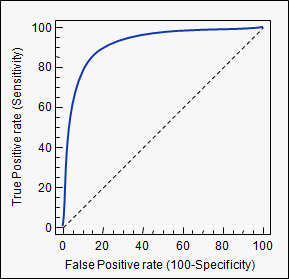
\includegraphics[width=2.5in, height=2in]{roc.png}
 \caption{an example of an ROC curve}
 \label{roc_example}
\end{figure}

\end{comment}



%\subsubsection{Residual Analysis}


\subsection{Logistic Regression Models on Training Data }

\subsubsection{Logistic Regression Model for Enrollment Decision.} 

%\noindent \textit{Training and Testing Data fro Enrollment Decisions.} 
The data from academic years  2008-2009 to 2011-2012 is used as training data and the data from the  year 2012-2013 as testing data. The training data has 30,083 entries and the testing data has 5,260 entries. 

%\noindent \textit{Parameter Estimation for Logistic Regression Models for Enrollment Management} 
The summary statistics for major variables in the logistic regression selected by the backward stepwise selection for enrollment are shown in Table \ref{lr_summary}. In the table, the  "estimate" column reports the odds ratio obtained from logistic regression, and an entry with value larger (smaller) than 1 represents that as the corresponding value increases, the odds would  increase (decrease). For other fields, please see \citep{DesJardins2006, long2006regression}. 

\begin{table}[H]
\centering
\begin{adjustbox}{width=0.95\textwidth}
\begin{tabular}{|lccclccc|} \hline %\hline
                               & Estimate & Std. Error & z value  &
                                                           Pr(\textgreater|z|) & Signif & 2.50\% & 97.50\% \\ \hline
(Intercept)                     & 2.5934   & 0.1476     & 6.4600   & 0.0000    & ***         & 1.9423 & 3.4639  \\
GPA                             & 1.3405   & 0.0463     & 6.3300   & 0.0000    & ***         & 1.2242 & 1.468   \\
ACT                             & 0.9630   & 0.0038     & -9.8200  & 0.0000    & ***         & 0.9558 & 0.9703  \\
HS.PERCENTILE                   & 0.9906   & 0.0011     & -8.8100  & 0.0000    & ***         & 0.9885 & 0.9927  \\
%APP.COLLEGEED                   & 0.9429   & 0.0493     & -1.1900  & 0.2331    &             & 0.8561 & 1.0385  \\
%APP.COLLEGEEG                   & 1.3506   & 0.0468     & 6.4200   & 0.0000    & ***         & 1.2322 & 1.4806  \\
%APP.COLLEGELA                   & 0.9670   & 0.0424     & -0.7900  & 0.4283    &             & 0.8899 & 1.0508  \\
%APP.COLLEGEN                    & 1.0696   & 0.0456     & 1.4800   & 0.1398    &             & 0.9782 & 1.1696  \\
%APP.COLLEGESM                   & 1.0530   & 0.0447     & 1.1600   & 0.2472    &             & 0.9648 & 1.1494  \\
%APP.COLLEGEUC                   & 0.9684   & 0.0419     & -0.7700  & 0.4441    &             & 0.8921 & 1.0513  \\
DISTANCE.BIN02                  & 0.6498   & 0.0420     & -10.2600 & 0.0000    & ***         & 0.5983 & 0.7054  \\
DISTANCE.BIN03                  & 0.4996   & 0.0737     & -9.4100  & 0.0000    & ***         & 0.4323 & 0.5772  \\
DISTANCE.BIN04                  & 0.5819   & 0.0826     & -6.5600  & 0.0000    & ***         & 0.4949 & 0.6841  \\
DISTANCE.BIN05                  & 0.4346   & 0.0843     & -9.8900  & 0.0000    & ***         & 0.3683 & 0.5126  \\
DISTANCE.BIN06                  & 0.3029   & 0.1124     & -10.6200 & 0.0000    & ***         & 0.243  & 0.3776  \\
%HS.COUNTY.TIERTier2             & 0.8634   & 0.0495     & -2.9700  & 0.0030    & **          & 0.7836 & 0.9514  \\
%HS.COUNTY.TIERTier3             & 1.0881   & 0.0927     & 0.9100   & 0.3627    &             & 0.9073 & 1.305   \\
%HS.COUNTY.TIERTier4             & 0.6191   & 0.0803     & -5.9700  & 0.0000    & ***         & 0.529  & 0.7247  \\
%HS.COUNTY.TIERTier5             & 0.7649   & 0.1010     & -2.6500  & 0.0080    & **          & 0.6274 & 0.9324  \\
%HS.COUNTY.TIERTier6             & 0.8602   & 0.0791     & -1.9000  & 0.0570    & .           & 0.7366 & 1.0046  \\
PELL.GRANT                      & 1.0002   & 0.0000     & 27.5700  & 0.0000    & ***         & 1.0001 & 1.0002  \\
ETHNICITYAfricanAmerican & 1.0272   & 0.0870     & 0.3100   & 0.7581    &             & 0.8661 & 1.2182  \\
%ETHNICITYForeign                & 1.4361   & 1.0153     & 0.3600   & 0.7215    &             & 0.1679 & 12.2457 \\
%ETHNICITYHawaiian               & 1.7012   & 0.3974     & 1.3400   & 0.1813    &             & 0.7922 & 3.8216  \\
ETHNICITYHispanic               & 1.1814   & 0.1085     & 1.5400   & 0.1245    &             & 0.955  & 1.4614  \\
%ETHNICITYIndianAlaskan          & 1.3713   & 0.2534     & 1.2500   & 0.2128    &             & 0.8348 & 2.261   \\
%ETHNICITYTwoMore                & 1.7766   & 0.1061     & 5.4200   & 0.0000    & ***         & 1.4435 & 2.1877  \\
ETHNICITYOthers                & 0.4939   & 0.1265     & -5.5800  & 0.0000    & ***         & 0.3848 & 0.632   \\
ETHNICITYWhite                  & 1.3417   & 0.0816     & 3.6000   & 0.0003    & ***         & 1.1433 & 1.5746  \\
UNEMPLOYMENT.INDEX              & 0.9655   & 0.0059     & -5.9100  & 0.0000    & ***         & 0.9544 & 0.9768  \\
SCHOLARSHIP\_PER                & 1.4894   & 0.0933     & 4.2700   & 0.0000    & ***         & 1.2403 & 1.7883  \\
%\\
%\\
%AIC: 47044\\
%Degrees of Freedom: 35330 \\
%Null Deviance:      48952 \\
%Residual Deviance: 46980
%\\
\hline %\hline
\multicolumn{7}{l}{\scriptsize{$^{***} p=0.000$, $^{**} p<0.001$, $^*p<0.01$,$^{.}p<0.05$}}
\end{tabular}
\end{adjustbox}
\caption{Summary statistics of logistic regression for enrollment model}
\label{lr_summary}
\end{table}

In interpreting these results, however, care should be taken because of the existence of collinearity. At first glance, it seems puzzling that  applicants with lower ACT are less likely to enroll, that applicants with higher GPA are more likely to enroll, and that HS.PERCENTILE does not impact enrollment very much. This is likely because of the fact that HS.PERCENTILE, ACT, and GPA are highly correlated with each other, so their effects are masked in the model. 

If an applicant is underrepresented, they are  less likely to enroll. Distance bins except Bin 1 (closest) are all less inclined to  enroll. Scholarship (SCHOLARSHIP\_PER) has an impact on the  enrollment -- the more scholarship that one receives, the more likely one is to enroll.  The unemployment index (0.9847), representing economy, has  little positive impact on the enrollment.
  
\subsubsection{Logistic Regression Model for Graduation.}  
Table \ref{lr_summary2} shows the summary statistics of major variables in the logistic regression for the graduation model. The table is similarly organized to the logistic regression for enrollment models.  It seems to suggest that  GPA and scholarship both have significant impact on  graduation. The higher the GPA and the higher the scholarship a student is awarded, the more likely that the student will graduate. 

\begin{table}[H]
\centering
\caption{Summary statistics of logistic regression for graduation model}
\label{lr_summary2}
\begin{adjustbox}{width=0.95\textwidth}
\begin{tabular}{|llllllll|} \hline %\hline
Coefficients:                   & Estimate & Std. Error & z value & Pr(\textgreater|z|) & Significant & 5\%    & 95\%   \\
(Intercept)                     & 2.6008   & 0.1576     & 3.1800  & 0.0015      & **          & 1.2737 & 2.1390 \\
GPA                             & 2.6872   & 0.0505     & 7.9640  & 0.0000      & ***         & 1.3757 & 1.6242 \\
ACT                             & 2.3540   & 0.0042     & -7.5840 & 0.0000      & ***         & 0.9622 & 0.9755 \\
HS.PERCENTILE                   & 3.4288   & 0.0012     & -8.1700 & 0.0000      & ***         & 0.9886 & 0.9924 \\
%APP.COLLEGEED                   & 2.4349   & 0.0531     & -0.8630 & 0.3879     &             & 0.8753 & 1.0423 \\
%APP.COLLEGEEG                   & 2.6597   & 0.0506     & 4.4450  & 0.0000     & ***         & 1.1523 & 1.3610 \\
%APP.COLLEGELA                   & 2.6243   & 0.0458     & -1.2560 & 0.2090     &             & 0.8757 & 1.0180 \\
%APP.COLLEGEN                    & 2.4402   & 0.0492     & 1.0520  & 0.2929     &             & 0.9712 & 1.1420 \\
%APP.COLLEGESM                   & 1.8190   & 0.0483     & 0.9280  & 0.3532     &             & 0.9660 & 1.1323 \\
%APP.COLLEGEUC                   & 1.5408   & 0.0451     & -1.3450 & 0.1787     &             & 0.8740 & 1.0136 \\
DISTANCE.BIN02                  & 1.6403   & 0.0446     & -8.8600 & \textless2e-16     & ***         & 0.6256 & 0.7246 \\
DISTANCE.BIN03                  & 1.4453   & 0.0794     & -7.4110 & 0.0000     & ***         & 0.4870 & 0.6325 \\
DISTANCE.BIN04                  & 1.2751   & 0.0889     & -5.3070 & 0.0000     & ***         & 0.5391 & 0.7221 \\
DISTANCE.BIN05                  & 2.1893   & 0.0911     & -7.4790 & 0.0000     & ***         & 0.4356 & 0.5877 \\
DISTANCE.BIN06                  & 2.4776   & 0.1223     & -8.0080 & 0.0000     & ***         & 0.3073 & 0.4594 \\
HS.COUNTY.TIERTier2             & 1.6972   & 0.0534     & -3.9420 & 0.0001     & ***         & 0.7418 & 0.8844 \\
HS.COUNTY.TIERTier3             & 1.8727   & 0.1002     & 0.2980  & 0.7657     &             & 0.8738 & 1.2149 \\
HS.COUNTY.TIERTier4             & 2.0888   & 0.0873     & -5.9900 & 0.0000     & ***         & 0.5135 & 0.6844 \\
HS.COUNTY.TIERTier5             & 2.7186   & 0.1101     & -3.4020 & 0.0007     & ***         & 0.5736 & 0.8240 \\
HS.COUNTY.TIERTier6             & 2.3776   & 0.0859     & -3.0990 & 0.0019     & **          & 0.6652 & 0.8826 \\
PELL.GRANT     & 1.1828   & 0.0000     & 22.9390 & 0.0000     & ***& 1.0001 & 1.0002 \\
ETHNICITYBlackOrAfricanAmerican & 2.2082   & 0.0925     & 1.1540  & 0.2483     &             & 0.9558 & 1.2958 \\
%ETHNICITYForeign                & 2.5987   & 1.1780     & -0.6230 & 0.5331     &             & 0.0432 & 2.8233 \\
%ETHNICITYHawaiian               & 2.3044   & 0.4322     & 1.3140  & 0.1890     &             & 0.8720 & 3.6575 \\
ETHNICITYHispanic               & 4.2355   & 0.1170     & 1.8430  & 0.0654     & .           & 1.0234 & 1.5040 \\
%ETHNICITYIndianAlaskan          & 1.4693   & 0.2690     & 1.1760  & 0.2396     &             & 0.8799 & 2.1367 \\
%ETHNICITYTwoMore                & 3.1371   & 0.1151     & 5.4470  & 0.0000     & ***         & 1.5494 & 2.2628 \\
%ETHNICITYUnknown                & 2.5971   & 0.1364     & -6.5000 & 0.0000     & ***         & 0.3287 & 0.5149 \\
ETHNICITYWhite                  & 3.4567   & 0.0864     & 3.0690  & 0.0021     & **          & 1.1312 & 1.5032 \\
UNEMPLOYMENT.INDEX              & 1.0000   & 0.0060     & -9.7690 & \textless2e-16     & ***         & 0.9336 & 0.9522 \\
SCHOLARSHIP\_PER                & 1.0000   & 0.1010     & 5.1330  & 0.0000     & ***         & 1.4221 & 1.9823    \\
%\\
%AIC: 4722\\
%Degrees of Freedom: 3998 \\
%Null Deviance:      5494.2 \\
%Residual Deviance: 4684.1
%\\
\hline %\hline
\multicolumn{7}{l}{\scriptsize{$^{***} p=0.000$, $^{**} p<0.001$, $^*p<0.01$,$^{.}p<0.05$}}

\end{tabular}
\end{adjustbox}
\end{table}

\subsection{Logistic Regression Tree Models on Training Data }
\subsubsection{Logistic Regression Tree Methodology }
A logistic regression tree model extends the baseline logistic regression  model and uses a \textit{divide and conquer} strategy to divide a complex set 
of data into many subsets such that a logistic regression model adequately fits the data in each subset. The division of the data into subsets is  performed recursively, one variable at a time, and results in the partitions of a binary decision tree \citep{harrell2013regression_book}.

The logistic tree with unbiased selection (LOTUS) algorithm \citep{lotus2}  is  selected in this research for the automation of a logistic regression tree. 
LOTUS allows  nonlinear features of the data sets to be modeled without  transforming the variables and compares favorably with standard stepwise 
logistic regression \citep{lotus_app1,lotus_app2}. The LOTUS implementation of the logistic regression tree is used in this analysis; for details, please see \citep{lotus2}.

\subsubsection{Logistic Regression Tree Models }
Two logistic regression trees are constructed: one for  enrollment, one for graduation.  In the construction of these tree models, the variables used in these two tree models and their role in the tree models  are listed in the table below. Here, ``D" represents the dependent variable, ``S '' is 
used as a numerical variable to split the tree, ``C'' represents categorical  variables to split the tree, ``X'' represents variables to ignore, and ``F'' represents the decision variables used in the 
logistic regression function at the tree node. 

\begin{table}[H]
\centering
\begin{tabular}{|l|c|c|c|c|}
\hline %\hline
 %& \multicolumn{2}{c|}{Variables} & \multicolumn{2}{c|}{Variables} \\ \hline
\multicolumn{1}{|c|}{\multirow{2}{*}{Column}} & \multicolumn{2}{c|}{Enrollment}
& \multicolumn{2}{c|}{Graduation}                            \\ \cline{2-5}
\multicolumn{1}{|c|}{}                        & Name                          &
Type                     & Name                          & Type
\\ \hline
1                                             & Enrolled                      &
D                        & Enrolled                      & X
\\ \hline
2                                             & GPA                           &
S                        & GPA                           & S
\\ \hline
3      & Tier   & C    &   Tier   & C    \\ \hline
4    & Raider     & C   &   Raider  & C   \\ \hline
5   & ACT    & S  &  ACT    & S     \\ \hline
6   & Underrepresented & C     & Underrepresented    & C   \\ \hline
7    & Gender   & C   &  Gender  & C   \\ \hline
8   & Ethnicity    & C     & Ethnicity   & C      \\ \hline
9   & Scholarship(\$)    & F   & Scholarship(\$)     & F    \\ \hline
10  & Scholarship(\%)   & F     & Scholarship(\%)     & F  \\ \hline
%11  & Estimated Tuition  & S    & Estimated Tuition  & S   \\ \hline
11  & Graduate   & X     &   Graduate        & D         \\ \hline

\end{tabular}
\caption{Variables used in the logistic regression tree models}
\end{table}

\subsection{Prediction Accuracy on Test Data}
\subsubsection{A. Logistic Regression and Logistic Regression Tree Models }
The logistic regression model and logistic regression tree models derived from the test data are applied to the test data to verify the accuracy of the models.  The cut-off value for enrollment is set to 0.5. So if  $p(x) \geq 0.5$, then enroll;  otherwise, not enroll.   

For the logistic regression model for enrollment prediction, the accuracy of the logistic regression model is 0.619 while the AUC is 0.658, as seen Table \ref{enroll_accuracy_model}. For the logistic regression model for graduation prediction, the accuracy of the logistic regression model is 0.74 while the AUC is 0.79, and seen in Table \ref{grad_accuracy_table}.
  
  \begin{table}[H]
  \centering
  \begin{threeparttable}
  \begin{tabular}{|l|c|c|l|l|l|}
  \hline
  \multicolumn{1}{|c|}{Model}          & \multicolumn{1}{l|}{AUC} & Accuracy
  & Enrolled                                                          &
    \begin{tabular}[c]{@{}l@{}}True Positive/\\ Negative Rate\end{tabular} &
    \begin{tabular}[c]{@{}l@{}}False Positive/\\ Negative Rate\end{tabular} \\
  \hline
  \multirow{2}{*}{Logistic Regression} & \multirow{2}{*}{0.658}   &
    \multirow{2}{*}{0.619 \tnote{*} } &
    \multirow{2}{*}{\begin{tabular}[c]{@{}l@{}}Yes\\ No\end{tabular}}    & 0.646 &
    0.414                 \\
  \cline{5-6} &  &   &  & 0.586            & 0.354
  \\ \hline
  
  \multirow{2}{*}{Logistic Regression Tree} & \multirow{2}{*}{0.618}   &
    \multirow{2}{*}{0.62 \tnote{*} } &
    \multirow{2}{*}{\begin{tabular}[c]{@{}l@{}}Yes\\ No\end{tabular}}    & 0.65
  & 0.414                                                                      \\
  \cline{5-6} &  &   &  & 0.586          & 0.35
  \\ \hline
  \end{tabular}
  %\begin{tablenotes}\footnotesize
  %\item[*] 95\% CI
  %\end{tablenotes}
  \end{threeparttable}
  \caption{Enrollment prediction from logistic regression and logistic regression tree}
  \label{enroll_accuracy_model}
  \end{table}
  
    
    \begin{table}[H]
  \centering
  \begin{threeparttable}
  \begin{tabular}{|l|c|c|l|l|l|}
  \hline
  \multicolumn{1}{|c|}{Model}    & \multicolumn{1}{l|}{AUC} & Accuracy
  & Graduated                                                          &
    \begin{tabular}[c]{@{}l@{}}True Positive/\\ Negative Rate\end{tabular} &
    \begin{tabular}[c]{@{}l@{}}False Positive/\\ Negative Rate\end{tabular} \\
  \hline
  \multirow{2}{*}{Logistic Regression} & \multirow{2}{*}{0.79}   &
    \multirow{2}{*}{0.74 \tnote{*} } &
    \multirow{2}{*}{\begin{tabular}[c]{@{}l@{}}Yes\\ No\end{tabular}}    & 0.8 & 0.41 \\
  \cline{5-6} &  &   &  & 0.59            & 0.2 \\ \hline
  
  \multirow{2}{*}{Logistic Regression Tree} & \multirow{2}{*}{0.76}   &
    \multirow{2}{*}{0.739 \tnote{*} } &
    \multirow{2}{*}{\begin{tabular}[c]{@{}l@{}}Yes\\ No\end{tabular}}    & 0.88 & 0.57                                                                    \\
  \cline{5-6} &  &   &  & 0.43            & 0.12 \\ \hline
  
  \end{tabular}
  %\begin{tablenotes}\footnotesize
  %\item[*] 95\% CI
  %\end{tablenotes}
  \end{threeparttable}
  \caption{Graduation prediction from logistic regression and logistic regression tree}
  \label{grad_accuracy_table}
  \end{table}
    
%Rather than the use of 0.5 as the discrimination threshold,  a receiver operating characteristic (ROC) curve is used by plotting the true positive rate (TPR) against the false positive rate (FPR) at various threshold settings, let the discrimination threshold be $\theta$, which ranges from 0 to 1,  the ROC curve is presented in Fig \ref{log_ROC}. %Here, for example, when $\theta = 0.5$, it shows that ....etc.   when $\theta = 0.5$, it shows that ....etc. ...

% \begin{figure}[!ht]
%   \centering
% 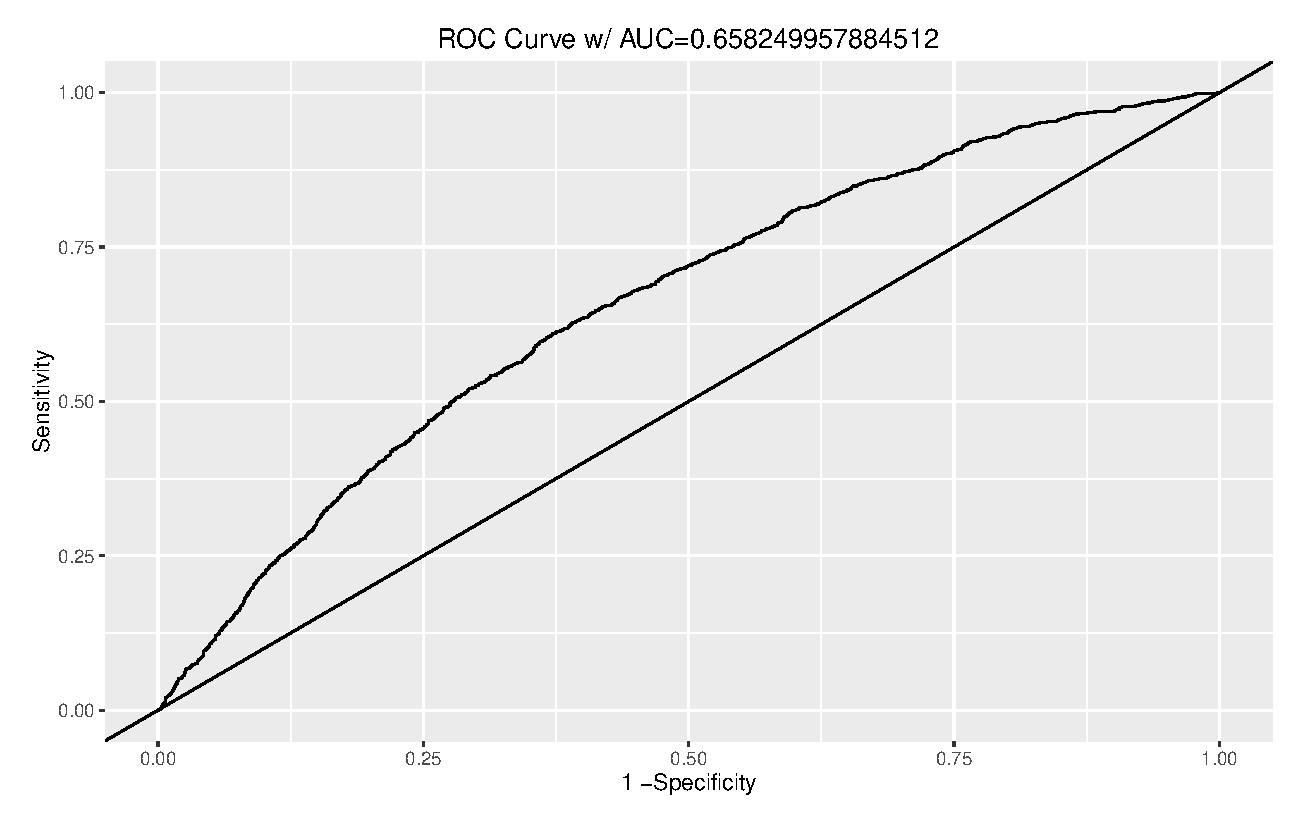
\includegraphics[width=6in, height=5in]{pic/model_roc.eps}
% \caption{ROC Curve of the Logistic Model }
% \label{log_ROC}
% \end{figure}


\subsubsection{B. Support Vector Machines and Neural Networks}
Preliminary experience with other logistic based models such as support vector machines and neural networks suggest similar accuracy results. The accuracy of 
prediction of these models are shown in the Table \ref{accuracy_model_enrollment_svm} and \ref{grad_accuracy_table_nn}.

\begin{table}[H]
\centering
\begin{threeparttable}
\begin{tabular}{|l|c|c|l|l|l|}
\hline
\multicolumn{1}{|c|}{Model}          & \multicolumn{1}{l|}{AUC} & Accuracy
& Enrolled                                                          &
\begin{tabular}[c]{@{}l@{}}True Positive/\\ Negative Rate\end{tabular} &
\begin{tabular}[c]{@{}l@{}}False Positive/\\ Negative Rate\end{tabular} \\
\hline
\multirow{2}{*}{Support Vector Machine} & \multirow{2}{*}{0.612}   &
\multirow{2}{*}{0.608 \tnote{*} } &
\multirow{2}{*}{\begin{tabular}[c]{@{}l@{}}Yes\\ No\end{tabular}}    & 0.531
& 0.306                                                                     \\
\cline{5-6} &  &   &  & 0.694            & 0.469 \\ \hline

\multirow{2}{*}{Neural Network} & \multirow{2}{*}{0.611}   &
\multirow{2}{*}{0.616 \tnote{*} } &
\multirow{2}{*}{\begin{tabular}[c]{@{}l@{}}Yes\\ No\end{tabular}}    & 0.647
& 0.425                                                                     \\
\cline{5-6} &  &   &  & 0.575            & 0.353 \\ \hline

\end{tabular}
%\begin{tablenotes}\footnotesize
%\item[*] 95\% CI
%\end{tablenotes}
\end{threeparttable}
\caption{Accuracy of enrollment prediction from support vector machine  and neural networks}
\label{accuracy_model_enrollment_svm}
\end{table}


\begin{comment}
\begin{table}[!ht]
\centering
\begin{threeparttable}
\begin{tabular}{|l|c|c|l|l|l|}
\hline
\multicolumn{1}{|c|}{Model}          & \multicolumn{1}{l|}{AUC} & Accuracy
& Enrolled                                                          &
\begin{tabular}[c]{@{}l@{}}True Positive/\\ Negative Rate\end{tabular} &
\begin{tabular}[c]{@{}l@{}}False Positive/\\ Negative Rate\end{tabular} \\
\hline
\multirow{2}{*}{Support Vector Machine} & \multirow{2}{*}{---}   &
\multirow{2}{*}{--- \tnote{*} } &
\multirow{2}{*}{\begin{tabular}[c]{@{}l@{}}Yes\\ No\end{tabular}}    & ----
& ----                                                                     \\
\cline{5-6} &  &   &  & ----            & ---- \\ \hline
\end{tabular}
\begin{tablenotes}\footnotesize
\item[*] 95\% CI
\end{tablenotes}
\end{threeparttable}
\caption{Accuracy of Graduation Prediction from Support Vector MachineModel }
\label{accuracy_model_graduation_svm}
\end{table}
\end{comment}

\begin{table}[H]
\centering
\begin{threeparttable}
\begin{tabular}{|l|c|c|l|l|l|}
\hline
\multicolumn{1}{|c|}{Model}    & \multicolumn{1}{l|}{AUC} & Accuracy
& Graduated                                                          &
\begin{tabular}[c]{@{}l@{}}True Positive/\\ Negative Rate\end{tabular} &
\begin{tabular}[c]{@{}l@{}}False Positive/\\ Negative Rate\end{tabular} \\
\hline
\multirow{2}{*}{Support Vector Machine} & \multirow{2}{*}{0.66}   &
\multirow{2}{*}{0.72 \tnote{*} } &
\multirow{2}{*}{\begin{tabular}[c]{@{}l@{}}Yes\\ No\end{tabular}}    & 0.77
& 0.230                                                                    \\
\cline{5-6} &  &   &  & 0.57            & 0.43 \\ \hline

\multirow{2}{*}{Neural Network} & \multirow{2}{*}{0.68}   &
\multirow{2}{*}{0.737 \tnote{*} } &
\multirow{2}{*}{\begin{tabular}[c]{@{}l@{}}Yes\\ No\end{tabular}}    & 0.78
& 0.22                                                                   \\
\cline{5-6} &  &   &  & 0.60            & 0.40 \\ \hline

\end{tabular}
%\begin{tablenotes}\footnotesize
%\item[*] 95\% CI
%\end{tablenotes}
\end{threeparttable}
\caption{Accuracy of graduation prediction from support vector machine and neural network}
\label{grad_accuracy_table_nn}
\end{table}

Due to space limitations, details of these models are not represented. To further develop these models to increase the prediction accuracy is the focus
of future study.

\section{ Answer to Enrollment \& Graduation Probabilities}
The predictions of enrollment probabilities for six applications with  different levels of scholarship awards are listed in Table 
\ref{prediction_sample}. 

\begin{table}[H]
\centering
 \small
 \setlength\tabcolsep{4pt}
    \begin{tabular}{|c|c|c|c|c|c|c|c|c|c|c|c|}
    \hline %\hline
    \multicolumn{12}{ |c| }{GPA 2.9, ACT 19 }  \\ \hline
& Student               & 0       & 1000    & 2000    & 3000    & 4000    &5000    & 6000    & 7000    & 8000    & 10000   \\ \hline
1& 2.9-Tier1-19-White    & 59.55 & 64.63 & 69.39 & 73.77 & 77.73 & 81.24 & 84.31 & 86.96 & 89.22 & 91.72 \\ \hline
2& 2.9-Tier5-19-White    & 36.96 & 40.20 & 43.53 & 46.92 & 50.34 & 53.75 & 57.13 & 60.45 & 63.67 & 69.74 \\ \hline
     \multicolumn{12}{ |c| }{GPA 3.3, ACT  25 }   \\ \hline
3& 3.3-Tier1-25-Hispanic & 23.80 & 27.44 & 31.42 & 35.69 & 40.20 & 44.88 & 49.65 & 54.43 & 59.13 & 67.97 \\ \hline
4& 3.3-Tier1-25-White    & 55.60 & 59.32 & 62.94 & 66.42 & 69.72 & 72.84 &75.75 & 78.43 & 80.90 & 85.17 \\ \hline
    \multicolumn{12}{ |c| }{GPA 3.8, ACT 28 }     \\ \hline
5& 3.8-Tier1-28-White    & 42.29 & 46.05 & 49.85 & 53.65 & 57.41 & 61.08 &64.63 & 68.03 & 71.25 & 77.07 \\ \hline
6& 3.8-Tier4-28-White    & 20.54 & 22.87 & 25.37 & 28.05 & 30.89 & 33.89 &37.02 & 40.26 & 43.60 & 50.41 \\ \hline
    \end{tabular}
\caption{Prediction of enrollment under different levels of  scholarships}
\label{prediction_sample}
\end{table}

Here, the concatenated string under ``student''  represents the characteristic of the student. For example, student ``2.9-Tier1-19-White'' represents an application from a student with a high school  GPA of 2.9, ACT score of 19, lives in Tier 1 region, and is of  the white. The number represents the probability of enrollment given the corresponding scholarship award, which spends from \$0 to \$10,000.

\vspace{0.15in}
\noindent \textbf{Observations.} Several interesting observations can be seen from these predictions, a) as GPA  increases, the probability of enrollment decreases; b) local students (Tier 1)  have a larger probability of enrollment than distance students (other tiers);  c) as financial aid increases, the probability of enrollment increases, yet  increase in probability with respect to scholarship is different among  different student groups.

\begin{itemize}
\item	Students 1 and 2: both students have the same GPA, ACT, and ethnicity, but student 1, who lives in Tier 1, has a much higher probability of enrollment than student 2, who lives in Tier 5.
\item Students 1 and 5: both students live in the same region and are of the same ethnicity, but student 1 (GPA of 2.9, ACT of 19) has a higher probability of enrollment than student 2 (GPA of 3.8 , ACT of 28).
\item Students 3 and 4: both students live in the same region and have the same GPA and ACT scores, but student 3 has a higher probability of enrollment than student 4 due to different ethnic backgrounds.
\end{itemize}

In all these cases, the probability of enrollment increases with the increase of scholarship awards. Though these observations are not surprising, accurate  quantitative prediction of these probabilities is essential to the allocation  of scholarship.

However, it  bears mentioning that the prediction of these probabilities alone  has not yet solved the fundamental problems for the enrollment management team  of any higher institution;  the optimal allocation of the scholarship to  optimize an institution's revenue, and the formation of concrete policies and  action plans,  needs to be solved. This is the second part of the research and  is addressed in the following sections.


\chapter {Prediction Models on the Number of Years of Study}
Recall that the net tuition of a student is the difference between tuition and scholarship, and the scholarship is renewable. This chapter studies the models to address the question on the number of years of study once a student enrolls in the university. 
% * <meiqingtian@gmail.com> 2017-11-19T21:22:45.597Z:
% 
% > scholarship
% scholarship varies over the years?
% 
% ^.

\section{Difference From a Retention Study}
It bears mentioning that the prediction on the number of years of study is is different from retention studies in most literature reviews. In retention studies, the focus is what factors influence the retention, and by doing analysis, early stage hazards can be identified to improve retention rate.
% * <meiqingtian@gmail.com> 2017-11-19T21:26:50.441Z:
% 
% > It bears mentioning
% is there another way to say this? you keep using the same phrase over and over.
% 
% ^.

Retention and dropout is affected by the interaction of students' pre-enrollment characteristics (academic performance, finance, ethnicity, etc.) and academic experience (peer group interactions, interaction with faculty, etc.) \citep{Tinto1975, Tinto1982, Terenzini1981}. Studies found that first-year students are the most vulnerable to drop out. Freshmen face drastic changes not only in  the form of the academic challenge but also all kinds of social challenges. Therefore retention of first-year students is mostly studied  \citep{Permzadian2016, Kovacic10earlyprediction, Horstmanshof2007, Noble2007}. Classification prediction methods such as logistic regression, decision tree, random forest, and neural networks were mostly used \citep{dekker2009, AdamGaither2005, quadri2010drop, yu2010data, Herzog2006, Lin2009,zhang2010using, Herzog2006}.

In a retention study, besides  pre-collegiate information, variables such as campus experience (on or off campus living, average class size, etc.), college academic performance (credit hours taken, grades, etc.), and ongoing financial need are critical.  In addition, health and psychosocial variables such as smoking, drinking, health-related quality of life and social support, were found significantly related to  academic achievement and retention \citep{deberard2004predictors, maney1990predicting, musgrave1997personality, cutrona1994perceived}. 

This study, however, is mainly focused on the use of pre-collegiate information such as demographics, high school academic performance, and financial background to predict the number of years study.  

\section{Methods and Results}
\subsection{Training and Testing Data}
In this study, only records of enrolled students  during  the 2006, 2007, and 2008 academic years were utilized, as the the latest data obtainedis Fall semester 2012 and the cutoff value for the study is graduation within 5 years.   Among the enrolled students, 43\% were male, 57\% were female;  73.9\% Caucasian, African American 17.8\%,  2.1\% Asian, 2\% Hispanic, 4.2\% Others. 

The training data of this study is from the years 2006-2007 and 2007-2008 when 3,999 students were enrolled. The testing data is from the year 2008-2009 when 2,355 students were enrolled. %Since the data collection ends at 2012-2013, the latest year of stay for testing data is 4.5 years. There are two types of matriculated students in the study: students leave the college with or without getting a degree. Students who graduate with a degree and without spending average 4.1 and 2.05 years respectively.
%The dependent variable for how long will stay has the following levels: 0, 0.5, 1, 1.5, 2, 2.5, 3, 3.5, 4, 4.5, 5. Students who stayed more than five years are removed from the analysis due to the rarity. Although the dependent variable is discreet, the problem is still a regression problem instead of a classification problem.
Variable selection for the number of years prediction is similar to the enrollment and graduation prediction. Again, unlike other studies \citep{Lin2009, deberard2004predictors, dekker2009}, which tracked the after enrollment data such as semester GPA and social activities, this research only used pre-collegiate variables due to data collection limit.

\begin{comment}
Table \ref{years_composite} shows the relation between average composite score and number of years of stay.
\end{}
\begin{figure}[ht]
   \centering
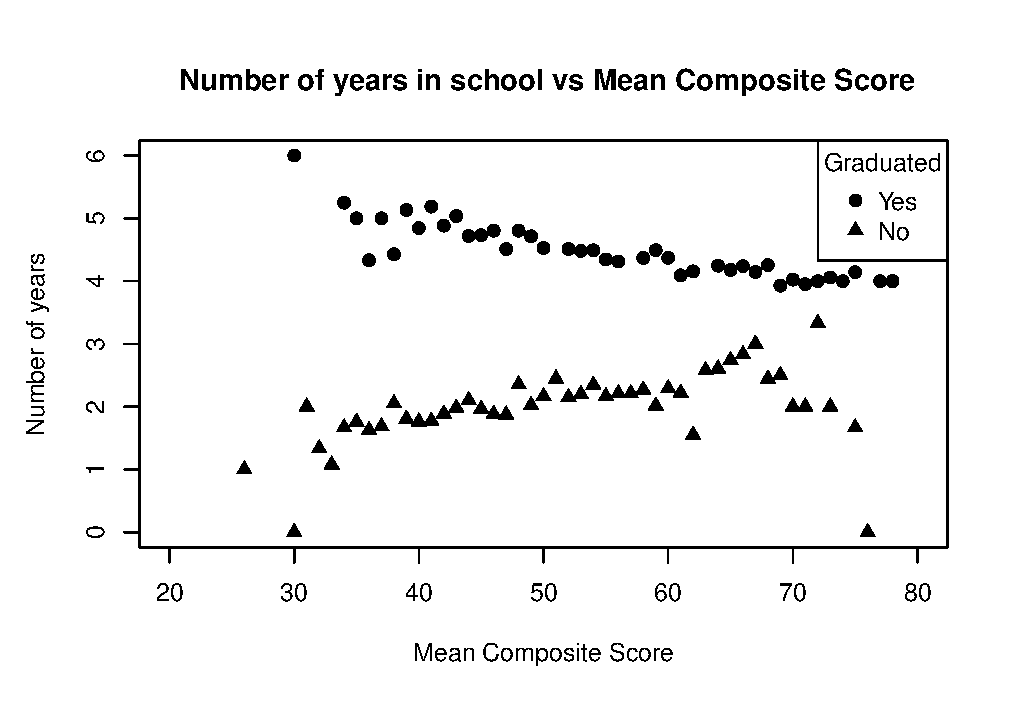
\includegraphics[width=5in,
height=3.5in]{pic/years_in_school_vs_composite_score.eps}
 \caption{Average Years in School vs Composite Score}
 \label{years_composite}
\end{figure}

\end{comment}

\subsection{Prediction Models}
Various data mining models such as linear regression, support vector machine regression, random forest, CART, and stochastic gradient boosting can be used to predict the number of years of study and provide ranks on the importance of the variable and are presented below.

%\subsubsection{Generalized Linear Model (GLM)}
\vspace{0.15in}
\noindent \textbf{Generalized Linear Model (GLM)} is a generalization of the linear regression model with a normally distributed dependent variable and Gaussian error. GLM broadens the distribution of the dependent variable to another family such as exponential or binomial. GLM can analyze interactions of variables, including mixtures of categorical and continuous variables.

\vspace{0.15in}
\noindent \textbf{Support Vector Machines (SVMs)} are supervised classifiers used for classification, regression and outliers detection. Given labeled data, the algorithm outputs an optimal hyperplane or set of hyperplanes, which separate the data into different classes. It also can be used for regression purposes.

Following is a simple two-dimensional example where the classes are linearly separable.  We have labeled example $(x_1,y_1)$,...,$(x_n, y_n)$ with label $y_i = 1$ for inputs $x_i$ in class 0 and $y_i = -1$ for inputs $x_i$ in class 1. The classification boundary or hyperplane is defined as $w^T x +b = 0$, where w is the weight vector and $b$ is the bias. The hyperplane can be represented by different scales of $(w,b)$. The optimal hyperplane is defined as $|w^T x +b | = 1$, where x is the data points closest to the hyperplane; for instance, the negative classification boundary is $w^T x +b = -1$ and positive classification boundary is $w^T x +b  = 1$. As a result, the distance between data point $x$ and the hyperplane $(w,b)$ is $ \frac{|w^T+b|}{||w||}= \frac{1}{||w||}$, so the total distance to positive and to negative class, defined as the margin $M$, is $\frac{2}{||w||}$.  The goal is to maximize margin $M$ to separate the data points valued 1 from those having -1, so we have to minimize the $w^T$. The final problem of linear SVM is to optimize:

\begin{equation}
\text{minimize} \ \frac{2}{||w||^2},
\text{ subject to }
y_{i}(w^T x +b) \geq 1 \ \forall i
\end{equation}
where $y_i$ is either positive class (1) or negative class (-1).

\vspace{0.15in}
\noindent \textbf{Support Vector Machine Regression (SVM regression)} is a sub-category of SVM to solve regression problems.  SVM regression performs linear regression in the high-dimension feature space using  $\epsilon$-insensitive loss and aims to reduce model complexity by minimizing $||w||^2$. By introducing slack variables $\xi$, the model is able to measure the error of training data outside the $\epsilon$-insensitive zone.
Thus,  SVM regression means solving the following minimization problem: 
\begin{equation}
    \begin{aligned}
     &   \text{minimize}
     & & \frac{1}{2} {||w||^2} + C \sum_{n=1}^{n}(\xi_i + \xi_i^+) \\
     & \text{subject to} 
     & & y_{i} - f(w,x_i) \leq  \epsilon + \xi^+, \\
     &&& f(w,x_i) - y_{i} \leq \epsilon + \xi, \\
     &&& \xi^i, \xi^+ \geq 0, i=1,\dots,n
    \end{aligned}
\end{equation}
where  $x_i$ is the training data and $y_i$ is target variable.
% * <meiqingtian@gmail.com> 2017-11-19T21:58:31.818Z:
% 
% left off here 11/19
% 
% ^.

\vspace{0.15in}
\noindent \textbf{Decision Trees} are commonly used to build classification and regression models in the form of tree-like  shapes. Decision tree methods separate data into groups to grow branches. A decision tree contains root nodes, terminal nodes, and internal nodes. The root node is the topmost node. Leaf nodes contain the final decision values of the dependent variable. Internal nodes represent the values of attributes. The algorithms used to build a decision tree include ID3, C4.5, C5.0, CHAID, CRUISE, etc. To split the tree, measurement algorithms like Gini index or information gain is used. For regression specifically, minimized  residual sum of squares (SSE):
% * <meiqingtian@gmail.com> 2017-11-22T02:53:43.603Z:
% 
% >  The root node is the one on the topmost, usually represented by the best attributes.
% I don't know what you're trying to say
% 
% ^ <meiqingtian@gmail.com> 2017-11-22T02:54:52.573Z.
\begin{equation}
    SSE = \sum_{i \in S_1} (y_i - \overline{y_1}) + \sum_{i \in S_2} (y_i - \overline{y_2})
\end{equation}
are used to split the value of an attribute. $\overline{y_1}$ and $\overline{y_2}$ are the average values of the dependent variables in group $S_1$ and $S_2$. 

\vspace{0.15in}
\noindent \textbf{Stochastic Gradient Boosting} is a sub-category of boosting methods which convert weak learners to strong learners. A boosting model works in the following way: starting with a base machine learning algorithm with a different distribution,  a second model is generated based on correcting errors from the first model. A decision tree with a fixed sized is typically used as the weak learner in the gradient boosting. The process iterates until the limit of the base algorithm is reached, or a certain accuracy is achieved. The estimate of response variables becomes consecutively more accurate between iterations. Stochastic gradient boosting for regression problems uses square error as a loss function. At each iteration, a sample of data was randomly selected from the full training data without replacement. The weaker learner then is built on the sample data instead of the full training data \citep{FRIEDMAN2002367}. 
% * <meiqingtian@gmail.com> 2017-11-22T03:03:41.838Z:
% 
% > different
% different from what?
% 
% ^.

\vspace{0.15in}
\noindent \textbf{Model Metrics.} To evaluate the performance of the model, the Root Mean Square Error (RMSE)  and the mean absolute error (MAE) are commonly used. 

RMSE is the square root of the average square of the difference between our predicted and actual values. RMSE is in the same units as the predicted value.
\begin{equation}
RMSE:  \sqrt{\frac{1}{n}\sum_{n=1}^n (y_i-\hat{y}_i)^2}
\end{equation}

MAE is used to measure the difference of forecasts to the real outcomes.
\begin{equation}
MAE = \frac{1}{n}\sum_{i=1}^n \left| y_i - \hat{y_i}\right| 
\end{equation}

\vspace{0.15in}
\textbf{Model Implementation.} For SVM regression, we used linear kernel in R (implemented in e1071 package \citep{e1071} using default settings). For GLM, we used the base function in R base package. For decision tree, we used rpart package \citep{rpart} in R. For stochastic gradient boosting, we used  gbm package in R \citep{gbm}.

\subsection{Experiment Results}
Two sets of experiments were conducted to evaluate the model's performance. The first experiment is 10-fold cross-validation. Data used in this experiment is from the year 2006-2007 and 2007-2008.  80\% of the data was randomly chosen to build the model, and 20\% percent of the data was used to validate the model in each fold. The final evaluation model is the average metric of all the folds. The second experiment is using data from 2008-2009 to predict the unseen students.  The results of the prediction models are as shown below:

\begin{table}[H]
\centering
\caption{Model results for 10 fold validation and validation on test data}
\label{num_year}
\begin{tabular}{|c|c|c|c|c|} \hline
                             & \multicolumn{2}{c|}{10-Fold Cross Validation} &
\multicolumn{2}{c|}{Test Data} \\ \hline
Model                        & RMSE                  & MAE                   & RMSE           & MAE           \\ \hline
GLM                          & 1.40                  & 1.2                   & 1.53           & 1.26          \\ \hline
SVM(Linear Kernel)           & 1.44                  & 1.20                  & 1.62           & 1.32          \\ \hline
Decision Tree                         & 1.43                  & 1.24        & 1.43           & 1.23          \\ \hline
Stochastic Gradient Boosting & 1.40                  & 1.19                  & 1.40           & 1.19           \\ \hline
\end{tabular}
\end{table}

The results show that the tree-based methods (decision trees and stochastic gradient boosting) yield slightly better results with lower RMSE and MAE for both 10-fold cross validation and validation based on test data.

\begin{table}[H]
\centering
\caption{Summary statistics of linear regression for number of years of study }
\label{LR_num_years}
\begin{adjustbox}{width=0.95\textwidth}
\begin{tabular}{|llllllll|} \hline %\hline
Coefficients:                   & Estimate & Std. Error & z value & Pr(\textgreater|z|) & Significant & 5\%    & 95\%   \\

(Intercept)                    &  -3.0276 & 1.3632  & -2.2  &  0.026 & *  &0.0033 & 0.7006 \\  
GPA                            &  0.73784 & 0.0510  & 14.5  & <2e-16 & ***&1.8922 & 2.3115 \\
ETHNICITYBlackOrAfricanAmerican&  0.12447 & 0.1744  &  0.7  &  0.475 &    &0.8046 & 1.5941 \\
ETHNICITYHawaiian              &  0.25884 & 1.0005 &   0.3  &  0.796 &    &0.1822 & 9.2056 \\
ETHNICITYHispanic              &  0.50478 & 0.2318 &   2.2  &  0.030 & *  &1.0517 & 2.6094 \\
ETHNICITYIndianAlaskan         &  0.01794 & 0.4061 &   0.0  &  0.965 &    &0.4431 & 2.1771 \\
ETHNICITYTwoMore               &  1.05399 & 0.2341 &   4.5  &  7e-06 & ***&1.8132 & 4.5396 \\
ETHNICITYUnknown               &  0.79924 & 0.2364 &  -3.4  &  7e-04 & ***&0.2828 & 0.7148 \\
ETHNICITYWhite                 &  0.03123 & 0.1623 &  -0.2  &  0.847 &    &0.7050 & 1.3323 \\
HS.COUNTY.TIERTier2            &  0.23719 & 0.0701 &  -3.4  &  7e-04 & ***&0.6874 & 0.9051 \\
HS.COUNTY.TIERTier3            &  0.08538 & 0.1217 &  -0.7  &  0.483 &    &0.7232 & 1.1656 \\
HS.COUNTY.TIERTier4            &  0.24058 & 0.0820 &  -2.9  &  0.003 & ** &0.6693 & 0.9233 \\
HS.COUNTY.TIERTier5            &  0.22394 & 0.0923 &  -2.4  &  0.015 & *  &0.6670 & 0.9579 \\
HS.COUNTY.TIERTier6            &  0.15317 & 0.0750 &  -2.0  &  0.041 & *  &0.7406 & 0.9938 \\
APP.COLLEGEED                  &  0.27311 & 0.1005 &  -2.7  &  0.007 & ** &0.6249 & 0.9267 \\
APP.COLLEGEEG                  &  0.12430 & 0.0956 &  -1.3  &  0.194 &    &0.7320 & 1.0652 \\
APP.COLLEGELA                  &  0.12102 & 0.0883 &  -1.4  &  0.171 &    &0.7450 & 1.0535 \\
APP.COLLEGEN                   &  0.33059 & 0.0972 &  -3.4  &  7e-04 & ***&0.5938 & 0.8693 \\
APP.COLLEGESM                  &  0.22383 & 0.0952 &  -2.4  &  0.019 & *  &0.6633 & 0.9635 \\
APP.COLLEGEUC                  &  0.17456 & 0.0857 &  -2.0  &  0.042 & *  &0.7099 & 0.9935 \\
OUT.OF.POCKET                  &  0.00004 & 0.0000 &   3.5  &  5e-04 & ***&1.0000 & 1.0000 \\
SCHOLARSHIP.PER                &  0.62733 & 0.2033 &   3.1  &  0.002 & ** &1.2570 & 2.7896 \\
UNEMPLOYMENT.INDEX             &  0.58469 & 0.2416 &   2.4  &  0.016 & *  &1.1175 & 2.8814 \\
%\\
%AIC: 4722\\
%Degrees of Freedom: 3998 \\
%Null Deviance:      5494.2 \\
%Residual Deviance: 4684.1
%\\
\hline %\hline
\multicolumn{7}{l}{\scriptsize{$^{***} p=0.000$, $^{**} p<0.001$, $^*p<0.01$,$^{.}p<0.05$}}

\end{tabular}
\end{adjustbox}
\end{table}
 

 
 
 
 
 
 
 
 
 
 
 
 
 
 
 
 
 
 
 
 
 
 





\vspace{0.15in}
\noindent \textbf{Variable Importance.} Finally, Table \ref{relatice_influ} presents the importance of variables in the prediction of number of years from a boosting model. %It seems to suggest that GPA, HS.PERCENTILE contribute the most to the model.

\begin{table}[H]
\centering
\caption{Relative influence of variables in gradient boosting model}
\label{relatice_influ}
\begin{tabular}{|c|c|} \hline
Variable                        & Relative Influence \\ \hline
GPA                             & 47.91771887        \\ \hline
HS.PERCENTILE                   & 12.9595027         \\ \hline
ACT                             & 7.050451247        \\ \hline
%ETHNICITYTwoMore                & 6.706346519        \\ \hline
PELL.GRANT                      & 4.743360342        \\ \hline
SCHOLARSHIP\_PER                & 4.033307548        \\ \hline
UNEMPLOYMENT.INDEX              & 3.202687597        \\ \hline
%ETHNICITYUnknown                & 2.83996864         \\ \hline
OUT.OF.POCKET                   & 1.770385883        \\ \hline
%ETHNICITYHispanic               & 1.68325614         \\ \hline
DISTANCE.BIN04                  & 1.251210899        \\ \hline
%COLLEGEN                    & 1.235771755        \\ \hline
DISTANCE.BIN05                  & 0.893538412        \\ \hline
DISTANCE.BIN02                  & 0.79644945         \\ \hline
DISTANCE.BIN03                  & 0.788177176        \\ \hline
%COLLEGEEG                   & 0.783195486        \\ \hline
ETHNICITYWhite                  & 0.542182288        \\ \hline
%COLLEGELA                   & 0.507483376        \\ \hline
%COLLEGESM                   & 0.295005675        \\ \hline
%COLLEGEED                   & 0                  \\ \hline
%COLLEGEUC                   & 0                  \\ \hline
%DISTANCE.BIN06                  & 0                  \\ \hline
%ETHNICITYBlackOrAfricanAmerican & 0                  \\ \hline
%ETHNICITYForeign                & 0                  \\ \hline
%ETHNICITYHawaiian               & 0                  \\ \hline
%ETHNICITYIndianAlaskan          & 0                  \\ \hline
\end{tabular}
\end{table}


\begin{comment}
\begin{figure}[ht]
   \centering
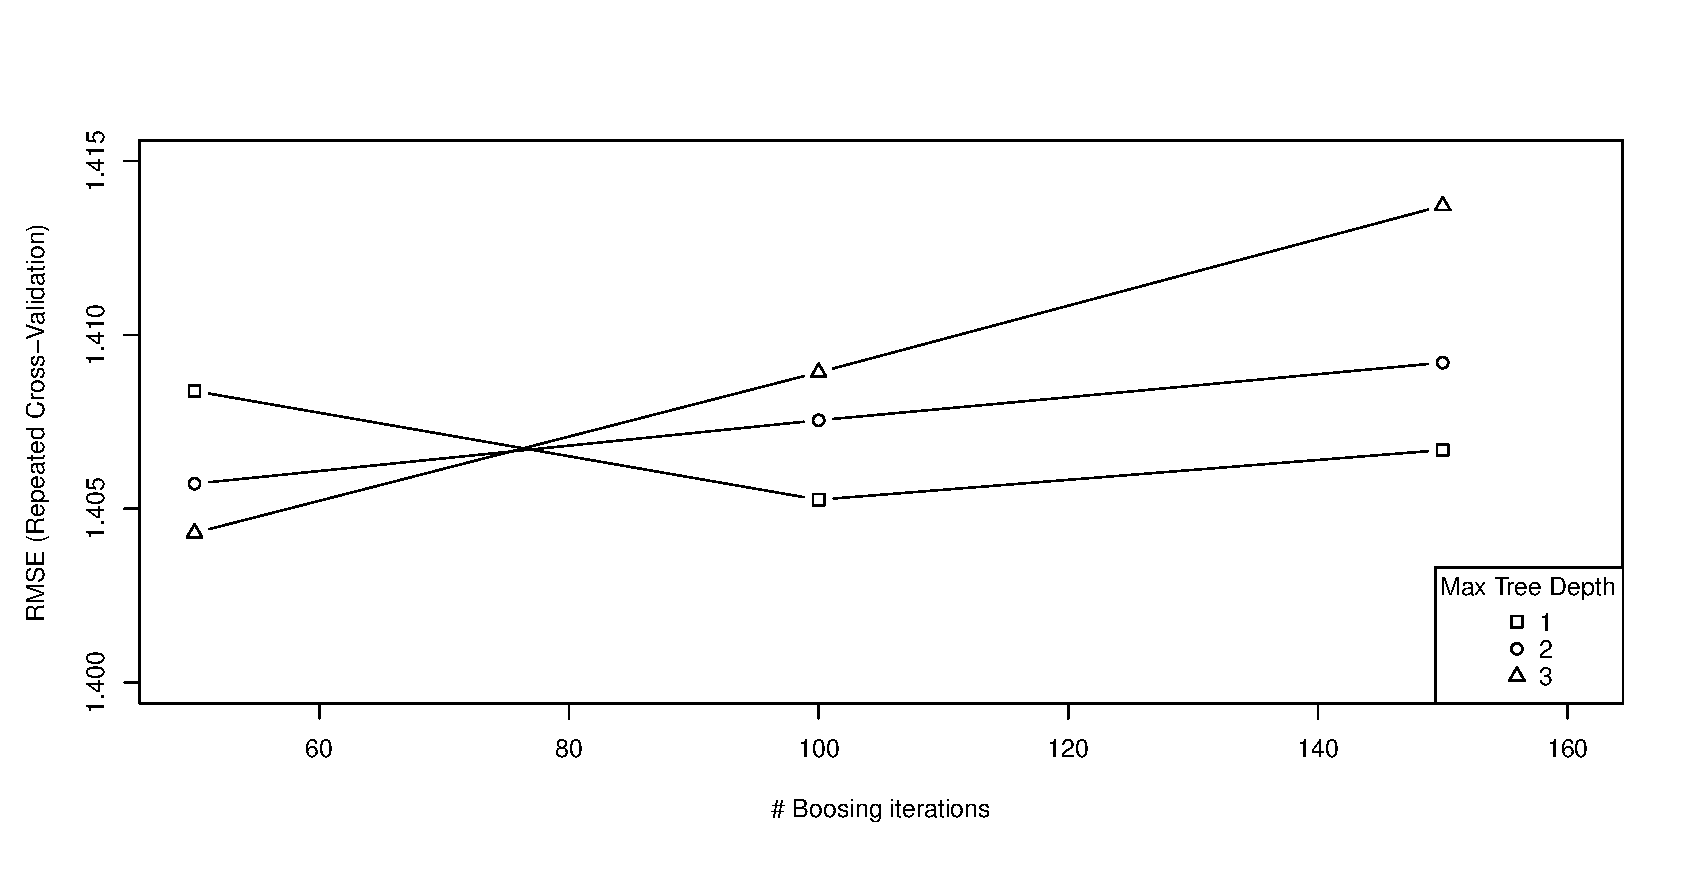
\includegraphics[width=5in,
height=3.5in,scale=0.5]{pic/Stochastic_boositing.eps}
 \caption{Stochastic booting procedure}
 \label{boosting}
\end{figure}
\end{comment}


\chapter{Mathematical Models for The Optimal Financial Aid  Allocation Problem }
The study of students' responses to scholarship awards, though it has provided many insights into the behavior of students in responding to awards, has not addressed the allocation of limited financial aid to students fundamentally.

For example, it is easy to see that local students require less money while students in far-away regions may need more money,  but it is still puzzling as: a) should we allocate the money to local students as they are our bread and butter students and require less money or b) should we allocate the money to far-away students as local students will come anyway? The solution to these problems requires the solution of an optimization problem to allocate the financial aid optimally, which is addressed in this chapter.

\section{The Financial Aid Optimization Model}
Given a set of applicants and their probabilities of enrollment and graduation with respect to different levels of financial aid, the optimization problem to be solved is to determine the financial aid to each applicant to  maximize the revenue. This is referred as the financial aid allocation problem.

In the development of the model, the following notations are used:
%------ define the list of set, variables, parameters
%------------------------------------
\newenvironment{conditions*}
  {\par\vspace{\abovedisplayskip}\noindent
\tabularx{\columnwidth}{>{$}l<{$} @{}>{${}}c<{{}$}@{}
>{\raggedright\arraybackslash}X}}
  {\endtabularx\par\vspace{\belowdisplayskip}}
%
%http://tex.stackexchange.com/questions/95838/how-to-write-a-perfect-equation
%-parameters-description
%---------------------------------------------------------------------  
\begin{conditions*}
\noindent\textbf{Sets}\\
I  \mbox{\qquad \qquad} &   & set of applicants,  indexed by $i$ and $j$ \\
M     &   & set of  different levels of financial awards, indexed by $m $\\
       &   &   $m \in  M = \{ 0,1000, 2000, \ldots ,8000\} $
\end{conditions*}
\vspace{-0.3in}

\begin{conditions*}
\textbf{Parameters}\\
p^e_{im}  & & probability of enrollment for applicant $i$, if given award $m$\\
p^g_{im}    & & probability of graduation for applicant $i$, if given award $m$\\
N_{im}    & & expected number of years student $i$ stays at the institution, if given award$m$  \\  
d(i,j)         & & 1 if applicant $i$ dominates applicant $j$; 0 otherwise.\\
B                & & total budget for financial aid\\
A_m              & &  monetary value of award $m$\\
T_i             & & tuition paid by applicant $i$\\
SSI_i     & & government compensation for applicant $i$ when he/she graduates\\

\textbf{Variables}\\
x_{im}           & & whether a financial award $m$ is allocated to applicant
$i$ or not\\
\end{conditions*}

\hspace{-0.5cm}\textbf{Objective}
\begin{align}
\max \quad
& \sum_{i\in I} \sum_{m\in M} x_{im}\cdot p^e_{im}\cdot(T_i-A_m)\cdot N_{im}+
\sum_{i\in I} \sum_{m\in M} x_{im}\cdot p^e_{im} \cdot p^g_{im}\cdot SSI_i
\label{objective}
\end{align}

\hspace{-0.55cm}\textbf{Subject to}
\begin{align}
\sum_{m \in M}x_{im}=1 &&   \forall i\in I \label{constraint:1}  \\
\sum_{i \in I} \sum_{m\in M} x_{im}\cdot p^e_{im}\cdot A_m\leq B
\label{constraint:2}  \\
\sum_{m \in M} x_{im}\cdot A_m \geq \sum_{m \in M} x_{jm}\cdot A_m && \forall
(i,j)|d(i,j)=1 \label{constraint:3}
\end{align}

The objective (\ref{objective}) is to maximize the total revenue. The first term represents the total tuition income from matriculated students, i.e., the tuition minus the award for each student, times the number of years of study; the second term represents the state compensation once the student graduates.

Constraint \ref{constraint:1}  states that each applicant is given one award (zero is an award with no monetary value). Constraint \ref{constraint:2} states that the total financial aid allocated cannot exceed the total budget B. Constraint  \ref{constraint:3} states that if applicant $i$ dominates applicant $j$, then applicant $i$ should be allocated a higher level award than applicant $j$.

\section{Model Size Reduction and Dominance Matrix}

\subsection{The Size of Pair-wise Dominance Constraints}
\noindent The size of the above model could be very large because of the number of pair-wise dominance relationships that form constraint \ref{constraint:3}.  For example, the university under study typically has more than 5,500 applicants each year; for each applicant $i$ and $j$ ($i \neq j$), there will be $(5,500 \times 5,500) / 2$ or more than 15 million constraints. Initial experiments with state-of-the-art commercial solvers were unsuccessful due to running out of memory.

However, if an applicant $i$ dominates applicant $k$, and applicant $k$ dominates applicant $j$, then it is only necessary to explicitly include domination constraints for applicants $i$ and $k$, as well as $k$ and $j$, but not necessarily for $i$ and $k$. The dominance constraint $i$ and $k$ is redundant as it is implicitly expressed in the other constraints.  In view of this, to reduce the size of the model, an efficient algorithm has been developed to find the domination matrix of minimum cardinality  without redundant dominance.

\subsection{Full Dominance Matrix}
The full dominance matrix between any applicant is defined first below. \textbf{Full (Direct) Dominance Matrix:} Let $D^{f}$ be an $n$ by $n$ matrix, where each element $d_{i,j}$ represents whether applicant $i$ dominates applicant $j$ or not. For simplicity,  dominance is only related to academic performance, for example:

\begin{equation}
   d_{i,j} =
  \begin{cases}
\quad   1   & \quad \mbox{if }  GPA_i \geq GPA_j \mbox{ and }  ACT_i \geq ACT_j
\\
  \quad   0  & \quad \mbox{otherwise}
  \end{cases}   
\end{equation}

\vspace{0.15in}
\noindent \textit{Example}:  Table \ref{student_sample} presents the ACT and GPA scores of six applicants.  Based on the above dominance definition, among these applicants, applicant 2 dominates 1, 4 and 5; applicant 3 dominates 1, 2, and 4; applicant 6 dominates applicants 1, 2, 4 and 5.


\begin{table}[H]
\centering
\begin{tabular}{|c|c|c|}
\hline
  Applicant & GPA & ACT \\ [0.5ex] 
\hline
1 & 2.9 & 18 \\ \hline
2 & 3.7 & 21 \\ \hline
3 & 3.8 & 30 \\ \hline
4 & 2.7 & 21 \\ \hline
5 & 3.3 & 17 \\ \hline
6 & 3.9 & 27 \\ \hline
\end{tabular}
\caption{An example  six students and their GPA and ACT scores} 
\label{student_sample}
\end{table}

These pairwise dominance relationships can be represented by graph and matrix forms shown in Figure \ref{full_domin}. Here, an arc between applicant $i$ and $j$ in the graph represents the dominance of applicant $i$ over $j$,  as is the entry of 1 in cell $(i,j)$ in the matrix form.


\begin{figure}
    \begin{floatrow}
        \ffigbox{%
            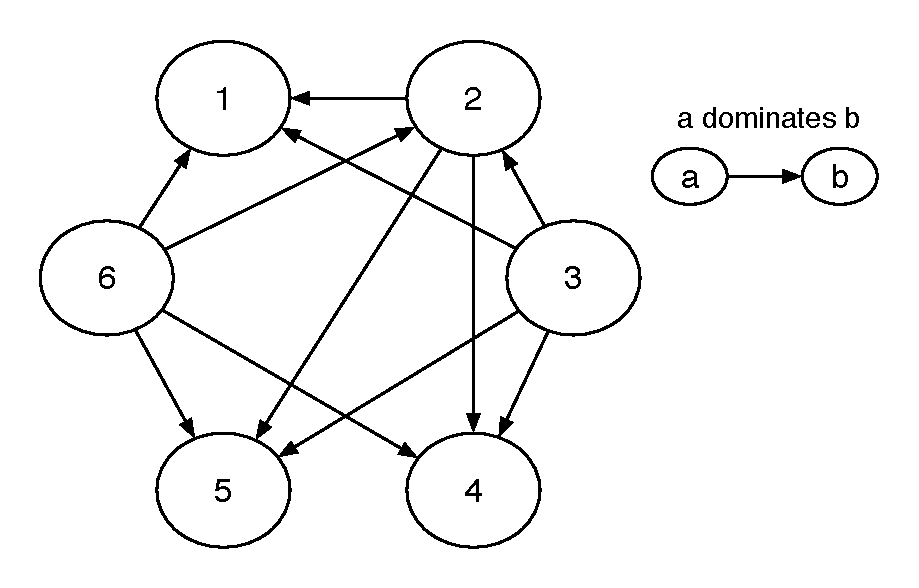
\includegraphics[scale=0.4]{pic/dominance1.eps}
        }{%
        \caption{Full dominance relationships in graph form}%
    }
    \capbtabbox
    }{%
    \caption{Full dominance relationships in matrix form}%
    \label{full_domin}
}
\end{floatrow}
\end{figure}


In this example, applicant 2 dominates applicant 1 and applicant 3 dominates applicant 2, so the dominance between applicant 3 and applicant 1 is redundant and can be eliminated.

\subsection{Redundant Dominance Matrix}
Graphically, a redundant relationship from node $i$ to node $j$ states that there exists at least one two-step path (not a direct path from node $i$ to node $j$) with one intermediate node, say from node $i$ to node $k$, and then from node $k$ to node $j$ (where $k$ can be any intermediate node).  The number of two-step paths from node $i$ to node $j$ with one intermediate node can be easily calculated by $$ \sum_k d(i,k) \cdot  d(k,j)$$ i.e., if there exists a redundant relationship, the inner product of the two corresponding vectors should be greater or equal to 1, and 0 otherwise.

The redundant relationship can thus be represented in a matrix, denoted as $D^2$,  as follows. $$D^2 = D^{f} \cdot D^{f} $$  Here $D^f$ is the original direct dominance matrix and  each entry in $D^2$ represents the number of two-step paths between a pair of applicants.
 
\noindent \textit{Example:} Applicant 2 dominates applicant 1, and applicant 3 dominates both applicants 1 and 2, therefore the entry $d_{21}=d_{31}=d_{32}=1$. The relationship between applicant 3 and the other applicants $k$ is: $d_{3k}=(1,1,0,1,1,0)$, and applicant 1 and the other applicants is $d_{k1}=(0,1,1,0,0,1) ^T $. Furthermore $\sum_k d_{3j} \cdot d_{k1}=d_{31}=1$. This represents that the relationship between applicants 1 and 3 is redundant.


\begin{figure}
\begin{floatrow}
    \ffigbox{%
        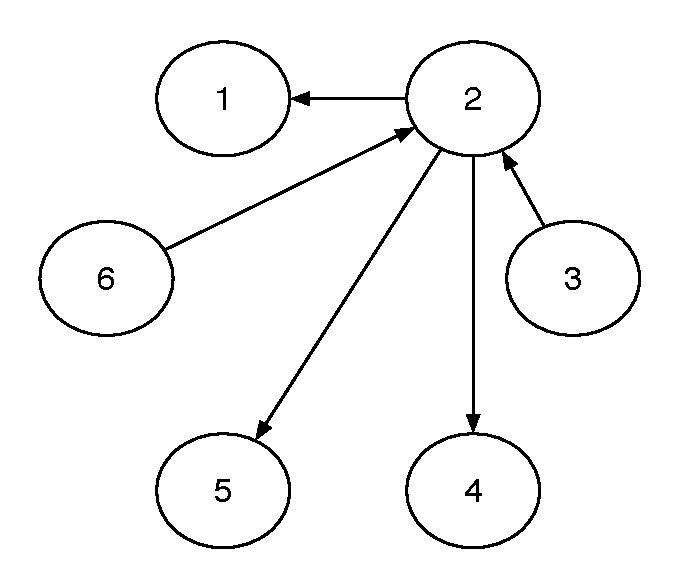
\includegraphics[scale=0.4]{pic/dominance3.eps}
        
    }{%
    \caption{Redundant dominance relationships in graph form}%
}
\capbtabbox
}{%
\caption{Redundant dominance relationships in matrix}%
\label{redundant1}
}
\end{floatrow}
\end{figure}


Finally, the elements of a \textbf{redundant matrix}, denoted as $ D_r$, can be defined as follows:
\begin{equation}
d^{r}_{i,j} =
  \begin{cases}
  \quad  1   & \quad if d^{2}_{i,j} >= 1 \\
  \quad  0  & \quad d^{2}_{i,j} = 0 
  \end{cases}   
\end{equation}

\subsection{Minimum Cardinality Dominance Matrix}
A minimum cardinality dominance matrix, defined as $D_m$, can be readily defined as: $$D_m = D_f - D_r $$

\vspace{0.15in}
\noindent \textit{Example:} By eliminating redundant relationships in the graph, the minimum dominance graph and matrix forms for the example are presented Figure \ref{redundant2}:

\begin{figure}
    \begin{floatrow}
        \ffigbox{%
            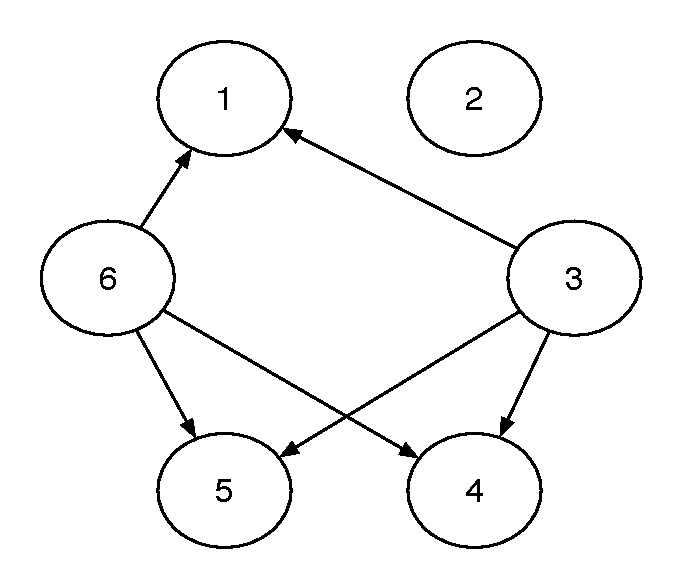
\includegraphics[scale=0.4]{pic/dominance2.eps}
        }{%
        \caption{Minimum dominance in graph form}%
    }
    \capbtabbox
    }{%
    \caption{Minimum dominance in matrix form}%
    \label{redundant2}
}
\end{floatrow}
\end{figure}


\section{Model Comparison and Results}
Computation experiments show that the use of minimum cardinality dominance has achieved a dramatic reduction in terms of model size.  To see this, Table \ref{model_comparison} presents the numbers of variables and constraints corresponding to each model. Here, though the number of variables has not changed, the number of constraints has been dramatically reduced, specifically the dominance constraint (\ref{constraint:2}), which comprises the largest part of the model. The original model has a total of 13,833,800 dominance constraints due to the use of a direct or full dominance matrix, the reduced model; however, has only 220,877 constraints.

\begin{table}[H]
\centering
\begin{tabular}{|c|l|c|c|}
\hline %\hline
\multicolumn{2}{|c|}{Model Components}     &
Original Model & Reduced Model \\ \hline
Variables                   & \multicolumn{1}{|l|}{Allocation (binary)  $x_i$}
& 57,860         & 57,860        \\ \hline
\multirow{3}{*}{Constraint} & One Award per ID  (\ref{constraint:1})        &
5,260          & 5,260         \\ \cline{2-4}
& Dominance  (\ref{constraint:2})    & 13,833,800   & 191,497
\\ \cline{2-4}
& Total Budget   (\ref{constraint:3})   & 1       & 1
\\ \cline{2-4}
& Total Number of Constraints                   & 13,839,061     & 196,758
\\ \hline
\end{tabular}
\caption{Size of the optimization models }
\label{model_comparison}
\label{size_model}
\end{table}

The solution of the original model with a state-of-the-art commercial solver is not possible due to memory limitations; the reduction model, however,  was solved in a few minutes on a standard laptop computer ( i7-4850HQ 2.3 GHz with 8G of RAM).

\subsection{Results Under Different SSI}
Table \ref{ssi10k}, Table \ref{ssi12k}, and Table \ref{ssi14k} show the optimization results for SSI set at 10000, 12000 and 14000 respectively.  Here  ``Integer Solution'' represents the integer solution value,  ``Linear Programming'' the linear programming solution values, ``Optimality Gap'' the optimality gap,  ``\# Nodes'' the number of nodes in the branch and bound tree,  and ``Time'' the time required in seconds to solve the problem. 

\begin{table}[H]
\centering
\caption{Computational statistics of optimization model under SSI=10,000}
\label{ssi10k}
\begin{tabular}{|c|c|c|c|c|c|}
\hline %\hline
SSI                          & \multicolumn{5}{c|}{10,000}                      
\\ \hline
\multicolumn{1}{|l|}{Budget} & \multicolumn{1}{l|}{Integer Solution} &
\multicolumn{1}{l|}{Linear Programming} & \multicolumn{1}{l|}{Optimality Gap} &
\multicolumn{1}{l|}{\# Nodes} & \multicolumn{1}{l|}{Time} \\
\hline
0.4M   & 61,516,543    & 61,527,360 & 0.02\%    & 0    &27                           \\ \hline
0.6M     & 61,552,340    & 61,559,211 & 0.01\%    & 181     &56                        \\ \hline
0.8M   & 61,584,196    & 61,594,905 & 0.02\%         & 45         &78                 \\ \hline
1.0M   & 61,603,302   & 61,616,648& 0.02\%     & 0     &27                          \\ \hline
1.2M   & 61,624,947    & 61,625,981& 0.00\%    & 0       &29                         \\ \hline
1.4M      & 61,606,891    & 61,618,654 & 0.02\%      & 0          & 108                  \\ \hline
1.6M    & 61,593,948      & 61,602,401 & 0.01\%      & 402     &431                      \\ \hline
1.8M       & 61,550,031         & 61,550,031 & 0.00\%         & 2270     &1080                 \\ \hline
2.0M       & 61,552,621       & 61,557,068 & 0.01\%      & 0          &133                   \\ \hline
2.2M     & 61,521,260       & 61,530,258 & 0.01\%    & 0     & 130                         \\ \hline
2.4M   & 61,472,929   & 61,495,934 & 0.04\%       & 0   &145                         \\ \hline
2.6M   & 61,428,352   & 61,455,128 & 0.04\%     & 80    &410                         \\ \hline
2.8M    & 61,414,620      & 61,416,969 & 0.00\%        & 0        &185                   \\ \hline
3.0M    & 61,350,350     & 61,361,072 & 0.02\%    & 32    & 209                         \\ \hline
3.2M    & 61,260,758  & 61,272,605 & 0.02\%   & 1444      &640                        \\ \hline
3.4M    & 61,185,830   & 61,197,559 & 0.02\%   & 598    & 373                          \\ \hline
\end{tabular}
\end{table}


\begin{table}[H]
\centering
\caption{Computational statistics of optimization model under SSI=12,000}
\label{ssi12k}
\begin{tabular}{|c|c|c|c|c|c|}
\hline   \hline
SSI     & \multicolumn{5}{c|}{12,000}                      
\\ \hline 
\multicolumn{1}{|l|}{Budget} & \multicolumn{1}{l|}{Integer Solution} &
\multicolumn{1}{l|}{Linear Programming} & \multicolumn{1}{l|}{Optimality Gap} &
\multicolumn{1}{l|}{\# Nodes} & \multicolumn{1}{l|}{Time} \\
\hline
1.4M   & 63,640,276         & 63,652,166           & 0.02\%         & 230           & 341  \\ \hline
1.6M   & 63,656,200         & 63,667,992           & 0.02\%         & 31           & 174  \\ \hline
1.8M   & 63,647,272         & 63,647,272           & 0.00\%         & 269          & 280  \\ \hline
2.0M   & 63,683,212         & 63,688,055           & 0.01\%         & 0            & 48   \\ \hline
2.2M   & 63,685,894         & 63,692,529           & 0.01\%         & 0            & 58   \\ \hline
2.4M   & 63,676,591         & 63,688,012           & 0.02\%         & 49           & 159  \\ \hline
2.6M   & 63,662,739         & 63,674,086           & 0.02\%         & 78           & 250  \\ \hline
2.8M   & 63,668,398         & 63,669,711           & 0.00\%         & 0            & 51   \\ \hline
3.0M   & 63,620,835         & 63,640,956           & 0.03\%         & 0            & 61   \\ \hline
3.2M   & 63,565,618         & 63,568,716           & 0.00\%         & 1190         & 806  \\ \hline
3.4M   & 63,523,681         & 63,526,856           & 0.00\%          & 529 		  & 323  \\ \hline
\end{tabular}
\end{table}

\begin{table}[H]
\centering
\caption{Computational statistics of optimization model under SSI=14,000}
\label{ssi14k}
\begin{tabular}{|c|c|c|c|c|c|}
\hline %\hline 
SSI     & \multicolumn{5}{c|}{14,000}                      
\\ \hline
\multicolumn{1}{|l|}{Budget} & \multicolumn{1}{l|}{Integer Solution} &
\multicolumn{1}{l|}{Linear Programming} & \multicolumn{1}{l|}{Optimality Gap} &
\multicolumn{1}{l|}{\# Nodes} & \multicolumn{1}{l|}{Time} \\
\hline
1.4M    & 65,673,717     & 65,686,331 & 0.02\%       & 256    &233                \\ \hline
1.6M   & 65,729,171  & 65,736,548 & 0.01\%   & 300     &202                    \\ \hline
1.8M   & 65,743,219   & 65,745,436 & 0.00\%       & 1191   & 470                \\ \hline
2.0M  & 65,815,085   & 65,819,285 & 0.01\%   & 0  & 107                        \\ \hline
2.2M   & 65,844,323   & 65,855,133 & 0.02\%     & 0  & 114                      \\ \hline
2.4M   & 65,871,923   & 65,877,439 & 0.01\%     & 2   & 224                     \\ \hline
2.6M      & 65,885,258     & 65,902,975 & 0.03\%     & 0       & 124                 \\ \hline
2.8M   & 65,919,822      & 65,923,025 & 0.00\%   & 0      & 49                     \\ \hline
3.0M    & 65,900,599    & 65,919,720 & 0.03\%   & 0    & 58                       \\ \hline
3.2M  & 65,871,018    & 65,874,012 & 0.00\%  & 808    & 451                     \\ \hline
3.4M      & 65,857,324     & 65,887,572 & 0.05\%   & 72    & 245                     \\ \hline
\end{tabular}
\end{table}

The plots of optimization results are shown in Figure \ref{ssi_10k_plot}, Figure \ref{ssi_12k_plot} and, Figure \ref{ssi_14k_plot}. The horizontal axis represents the budget and the vertical axis the revenue. 


\begin{figure}[ht]
    \centering
%    [width=5in, height=3.5in,scale=0.5]
    \includegraphics[width=6in,height=3in,scale=0.5]{pic/ssi_10k.eps}
    \caption{Optimization results for SSI = 10,000. }
     \label{ssi_10k_plot}
\end{figure}


\begin{figure}[ht]
    \centering
%    [width=5in, height=3.5in,scale=0.5]
    \includegraphics[width=6in, height=3in, scale=0.5]{pic/ssi_12k.eps}
    \caption{Optimization results for SSI = 12,000. }
     \label{ssi_12k_plot}
\end{figure}

\begin{figure}[ht]
    \centering
%    [width=5in, height=3.5in,scale=0.5]
    \includegraphics[width=6in, height=3in,scale=0.5]{pic/ssi_14k.eps}
    \caption{Optimization results for SSI = 14,000. }
     \label{ssi_14k_plot}
\end{figure}


As can be seen in Figure \ref{ssi_10k_plot}, for SSI = 10,000, a 1.2 million budget yields the maximum  revenue return; for SSI  = 12,000, a 2.2 million budget yields the maximum revenue; for SSI  = 14,000, a  2.8 million budget yields the maximum revenue.  In all these figures, revenue increases at the beginning  as more financial aid is being allocated and more students are likely to enroll. However, after the point  where maximum revenue is reached, additional financial aid negatively affects net tuition and reduces  revenue and thus is not desired.  


\begin{comment}
\begin{figure}[ht]
    \centering
%    [width=5in, height=3.5in,scale=0.5]
    \includegraphics[width=5in,height=2.5in,scale=0.3]{pic/ssi_14k.eps}
    \caption{Optimization results under different budget SSI=14k }
     \label{ssi_14k_plot}
\end{figure}
\end{comment}

% \begin{figure}[ht]
%    \centering
%    \includegraphics[width=5in,height=2.5in,scale=0.3]{pic/act_10k.eps}
% \end{figure}
% \begin{figure}[ht]
%    \centering
%    \includegraphics[width=5in,height=2.5in,scale=0.3]{pic/act_12k.eps}
% \end{figure}
% \begin{figure}[ht]
%    \centering
%    \includegraphics[width=5in,height=2.5in,scale=0.3]{pic/act_14k.eps}
% \end{figure}




\begin{comment}

\subsubsection {Extension with Program Capacity Variations}
University have various units or programs, and typically with various
capacities, that evolve over the years. Proactive marketing and optimization
would help to attract as many students as possible to a business unit with
capacity constraints, or minimal investment for a business unit with excess
capacity (before layoffs or attrition).  The following additional notation is
used in the development of capacity constraints.
\begin{conditions*}
U & &       \quad set of business units under study, indexed by u\\
I_u & &     \quad set of students who are interested in business unit u\\
N_u & &   \quad number of resources (such as faculty members) available for
unit u\\
C_u & &    \quad cost of a single resource\\
\rho_u & & \quad supervising  rate or faculty-to-student ratio for a single
resource in unit u\\
Z_u & &    \quad the additional resource to be hired for each business unit u
\end{conditions*}


\begin{align}
\sum_{i \in I_u}\sum_{m \in M} x_{i,m}\cdot p^e_{i,m}\leq \rho_u\cdot N_u +
\rho_u\cdot Z_u  && \forall u \in U
\end{align}

This constraint states that total number enrolled (left hand size) has to be
less than the current capacity of the program, plus additional hires if
necessary.  The new hires can be added to the objective function.

\end{comment}




%%%%%%%%%%%%%%%%%%%%%%%%%%%%%%%%%%%%%%%%

\chapter{Derivation of Scholarship Award Policies \& Implementation}

The optimization result based on the above model could be sent to a general linear regression or decision tree for analysis to derive scholarship award policies.  These policies represent a simplified solution to the optimal allocation problem; as such, in the development of these policies, it would be desirable that they are simple to understand and do not lose the optimality of allocation. 


\section{Derivation of Scholarship Award Policies}
Scholarship award policies can be derived using the above model, which is based on general linear regression or decision tree.  Here the predictor or dependent variable is the amount of the award, and the independent variables are GPA, ACT scores, etc.  Although variables such as gender could affect the enrollment and graduation probabilities,  aid allocation based on these variables is controversial. 
As a result, in the derivation of financial aid policies, variables such as gender, family income and ethnicity are not considered in the design of a merit-based scholarship.

\subsection{Scholarship Award Policy Based on Decision Tree }

The decision tree analysis is used in the derivation of  financial aid policies.  In the past two decades, decision trees, as a decision support tool, have been commonly used in various business domains, such as direct mailing, on-line sales, customer retention and supplier selection, to name a few \citep{Han2011}.

Decision tree analysis is a tree-structured model. There are three types of nodes in a decision tree: a) a root node that has no incoming edges; b) an internal node with one incoming edge and one or more outgoing edges; c) leaf node, which corresponds with a classification rule. Please see \citep{Maimon2005} for more details.

The financial aid policy initially obtained from the decision tree analysis is presented in Figure \ref{FApolicybyDT}.  For example, for a student with GPA = 4.0, ACT = 30, it passes to the right at the root node (ACT < 26.5, no),  then to the right at node (GPA <3.85, no), and then to the right at node (ACT <28.5, no),  which lands him at a scholarship of \$5,339;   for  for a student with GPA = 3.5, ACT = 28, it passes to the right at the root node (ACT < 26.5, No), then to the left at node (GPA <3.85, yes), and then to the left at node (ACT <29.5, no), then to the right at node (GPA<3,35, no), which lands him at a scholarship of \$2,306.

The decision tree analysis, though graphical, still seems a little complicated to reveal the intrinsic patterns of the award. 

\begin{sidewaysfigure}
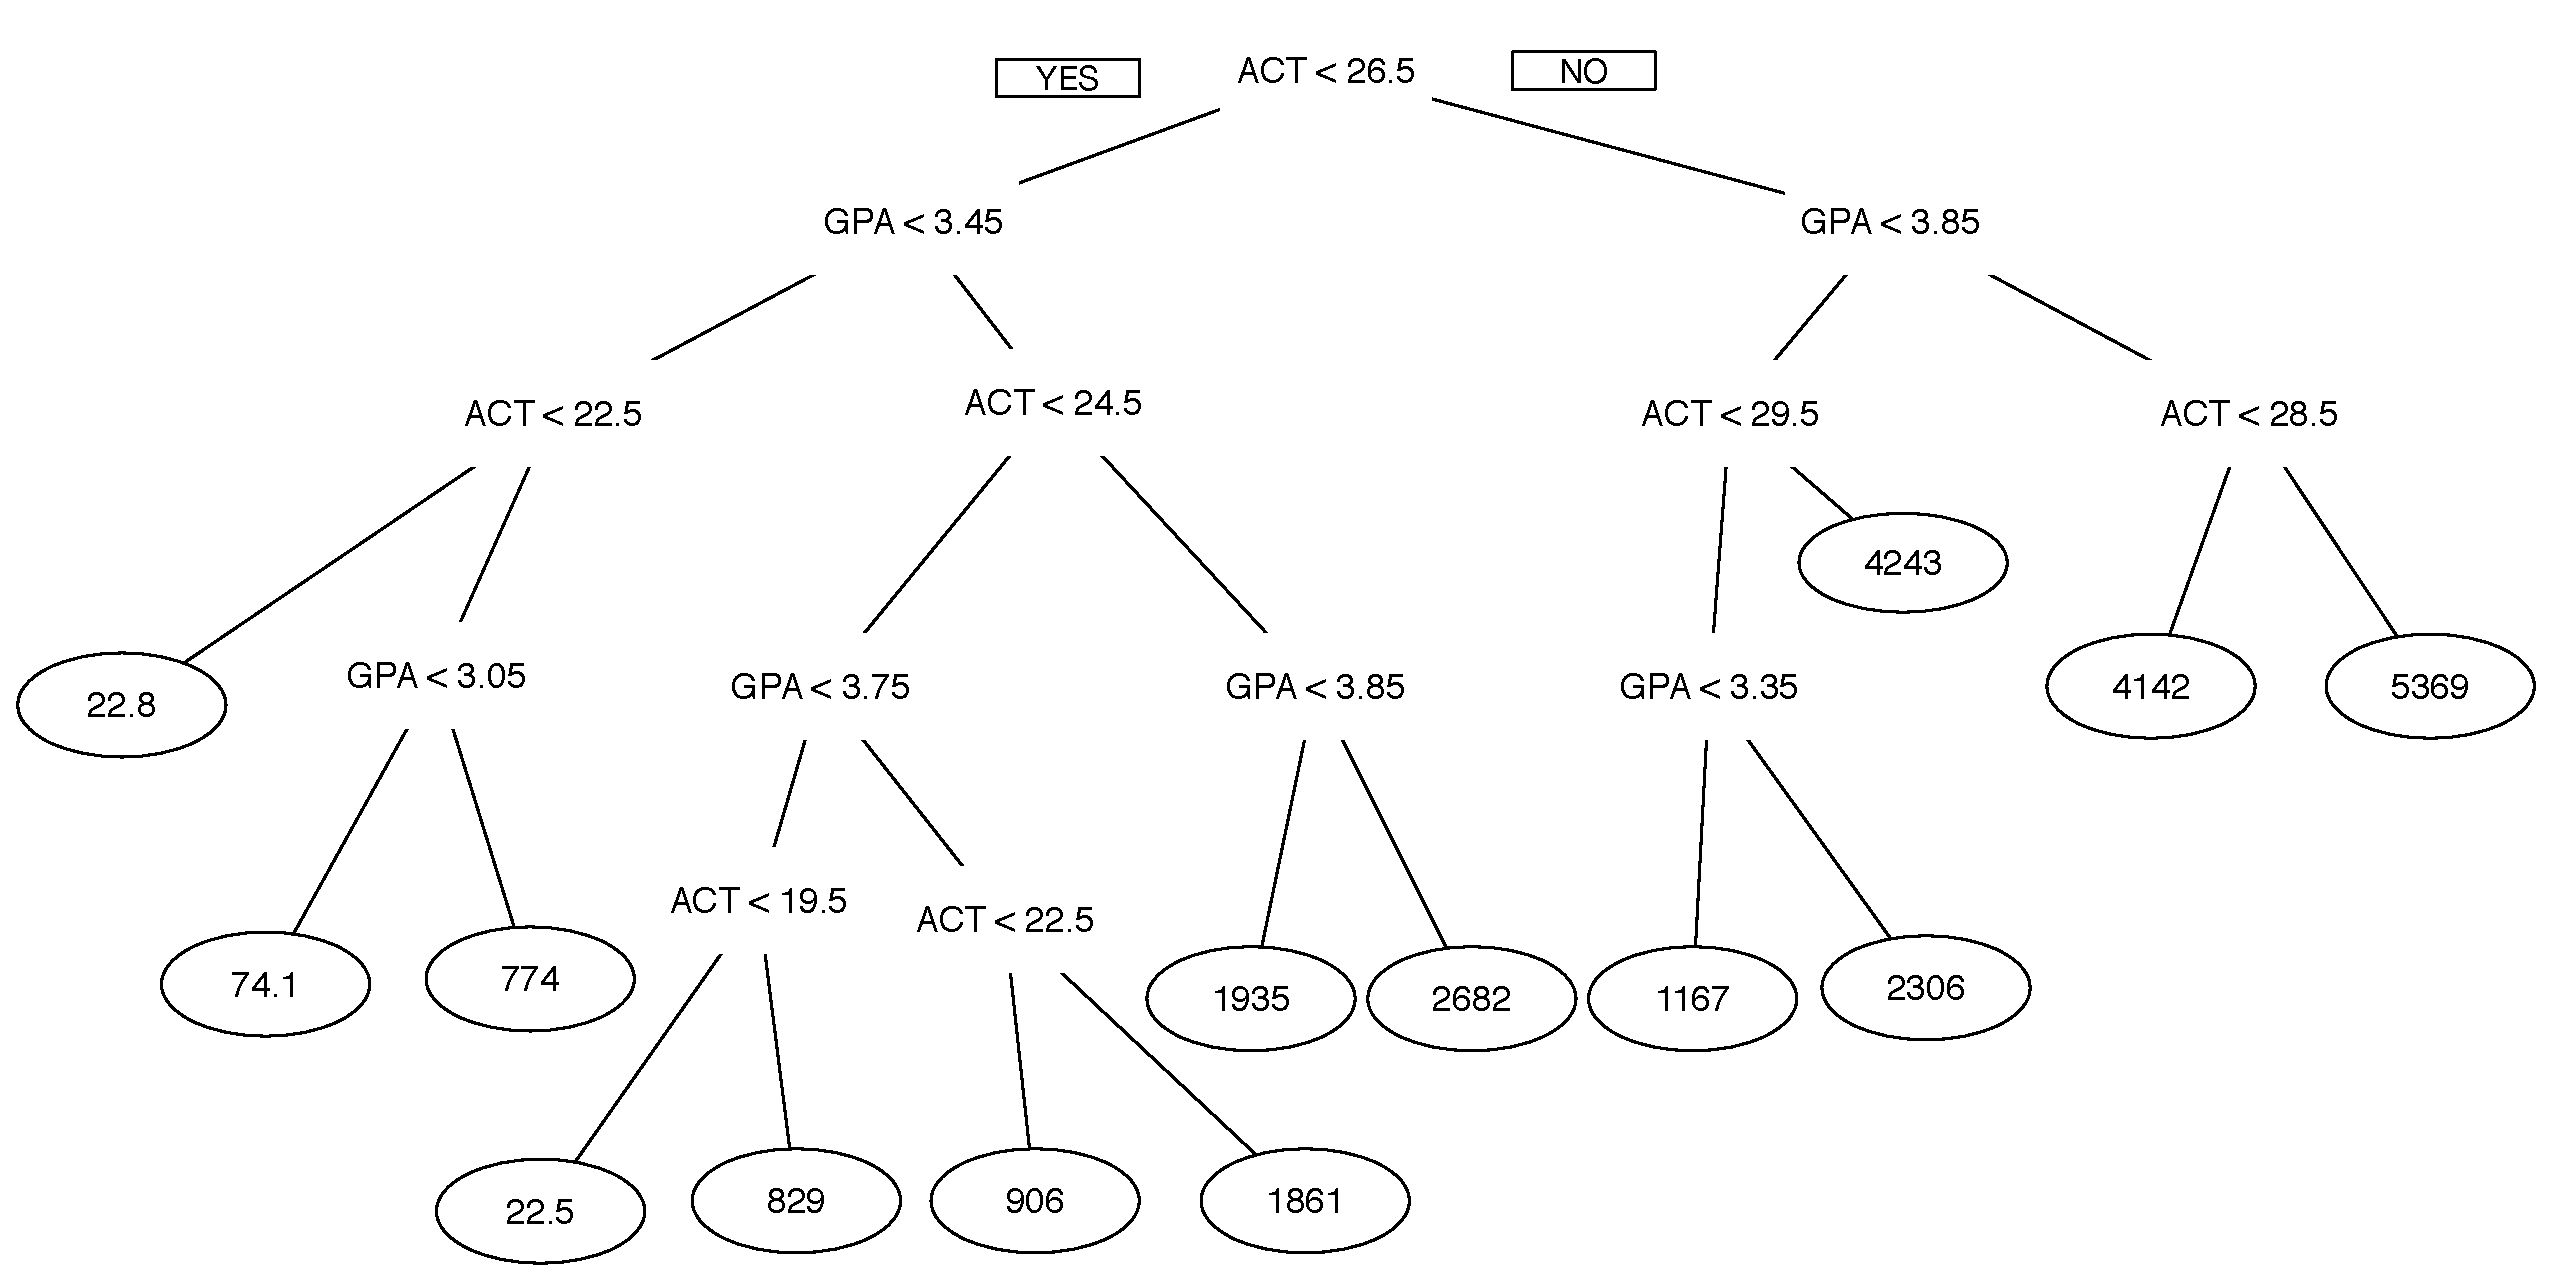
\includegraphics[width=6.5in, height=4.5in]{pic/FA_DT_Result.eps}%
\caption{Financial aid policy based on decision tree }
\label{FApolicybyDT}
\end{sidewaysfigure}
 
\subsection{Scholarship Award Policy on Stepwise Regression}
The more intuitive answer to the scholarship allocation from the optimization results is based on two observations; a) the composite score and 2) the piece-wise relations.  

\vspace{0.1in}
\noindent \textbf{1. Composite Score} 

\noindent Table \ref{opt_scholar_act} presents the average financial aid with respect to the students' GPA and ACT scores. Here the row names represent the GPA scores, and the column names represent the ACT scores. The average financial aid awarded (based on the optimal results with a scholarship budget of \$2.4 million) is shown in the corresponding grid.

These results suggest a strong relationship between the awards and both GPA and ACT scores. As a result, a \textit{composite score}, calculated as $10\times GPA + ACT $ was proposed by the enrollment team to capture the applicants' academic merits and used as the basis for the award.

\begin{sidewaystable}[!htbp]
 \resizebox{\linewidth}{175pt}{
\begin{tabular}{@{\extracolsep{5pt}} |l|cccccccccccccccccc|c|}
\hline
GPA/ACT  & \multicolumn{1}{c|}{18}     & \multicolumn{1}{c|}{19}
& \multicolumn{1}{c|}{20}          & \multicolumn{1}{c|}{21}          &
\multicolumn{1}{c|}{22}          & \multicolumn{1}{c|}{23}   &
\multicolumn{1}{c|}{24}          & \multicolumn{1}{c|}{25}          &
\multicolumn{1}{c|}{26}        & \multicolumn{1}{c|}{27}         &
\multicolumn{1}{c|}{28}          & \multicolumn{1}{c|}{29}          &
\multicolumn{1}{c|}{30}          & \multicolumn{1}{c|}{31}         &
\multicolumn{1}{c|}{32}          & \multicolumn{1}{c|}{33}          &
\multicolumn{1}{c|}{34}          & 35     & Total \\ \hline
1           &                                  &
&                                  &                                  &     &
&                                  &                                  &     &
&                                  &                                  &
&                                 &                                  &
&                                  &        & 0           \\ \cline{1-1}
\cline{20-20}
1.1         &                                  &
&                                  &                                  &
&                           &                                  &
&                                &                                 &
&                                  &                                  &
&                                  &                                  &
&        & 0           \\ \cline{1-1} \cline{20-20}
1.2         &                                  & 0
&                                  &                                  &
&                           &                                  &
&                                &                                 &
&                                  &                                  &
&                                  &                                  &
&        & 0           \\ \cline{1-1} \cline{20-20}
1.3         & 0                                &
&                                  &                                  &
&                           &                                  &
&                                &                                 &
&                                  &                                  &
&                                  &                                  &
&        & 0           \\ \cline{1-1} \cline{20-20}
1.4         &                                  & 0
&                                  &                                  &
&                           &                                  &
&                                &                                 &
&                                  &                                  &
&                                  &                                  &
&        & 0           \\ \cline{1-1} \cline{20-20}
1.5         &                                  & 0
&                                  &                                  &
&                           &                                  &
& 0                              &                                 &
&                                  &                                  &
&                                  &                                  &
&        & 0           \\ \cline{1-1} \cline{20-20}
2.5         & 0                                & 0
& 0                                & 0                                & 0
& 0                         & 0                                & 0
& 0                              & 0                               & 0
& 0                                &                                  & 0
&                                  &                                  &
&        & 0           \\ \cline{1-1} \cline{20-20}
2.6         & 0                                & 0
& 0                                & 0                                & 0
& 0                         & 0                                & 0
& 0                              & 0                               &
& 1250                             & 1500                             &
&                                  & 1500                             &
&        & 25.8 \\ \cline{1-1} \cline{20-20}
2.7         & 0                                & 0
& 0                                & 0                                & 0
& 0                         & 0                                & 0
& 0                              & 0                               & 1500
&                                  & 2000                             &
&                                  &                                  &
&        & 24.2 \\ \cline{1-1} \cline{20-20}
2.8         & 0                                & 0
& 0                                & 0                                & 0
& 0                         & 0                                & 0
& 0                              & 300                             & 1500
& 2000                             &                                  &
&                                  & 2500                             &
&        & 39.4 \\ \cline{1-1} \cline{20-20}
2.9         & 0.0                              & 0.0
& 0.0                              & 0.0                              & 0.0
& 0.0                       & 0.0                              & 0.0
& 818.2                          & 1875.0                          & 2000.0
&                                  &                                  &
&                                  &                                  &
&        & 63.4        \\ \cline{1-1} \cline{20-20}
3           & 0.0                              & 0.0
& 0.0                              & 0.0                              & 0.0
& 0.0                       & 0.0                              & 1166.7
& 1500.0                         & 2000.0                          & 2000.0
& 2200.0                           &                                  & 3200.0
&                                  &                                  & 5200.0
&        & 216.3       \\ \cline{1-1} \cline{20-20}
3.1         & 0.0                              & 0.0
& 0.0                              & 0.0                              & 0.0
& 0.0                       & 523.8                            & 1500.0
& 1727.3                         & 2000.0                          & 2000.0
& 2500.0                           & 2500.0                           &
&                                  &                                  &
& 7300.0 & 276.7       \\ \cline{1-1} \cline{20-20}
3.2         & 0.0                              & 0.0
& 0.0                              & 0.0                              & 0.0
& 781.3                     & 1000.0                           & 1750.0
& 2000.0                         & 2250.0                          & 2500.0
& 2500.0                           & 2780.0                           & 3950.0
& 5200.0                           &                                  &
&        & 573.7       \\ \cline{1-1} \cline{20-20}
3.3         & 0.0                              & 0.0
& 0.0                              & 0.0                              & 647.1
& 1000.0                    & 1613.6                           & 2000.0
& 2315.8                         & 2500.0                          & 2920.0
& 3200.0                           & 3866.7                           & 4200.0
&                                  & 5200.0                           & 5200.0
&        & 962.8       \\ \cline{1-1} \cline{20-20}
3.4         & 0.0                              & 0.0
& 0.0                              & 694.4                            & 1000.0
& 1550.0                    & 2000.0                           & 2000.0
& 2500.0                         & 2990.0                          & 3200.0
& 3200.0                           & 4200.0                           & 4200.0
&                                  &                                  &
&        & 1185.1      \\ \cline{1-1} \cline{20-20}
3.5         & 0.0                              & 0.0
& 695.7                            & 1000.0                           & 1724.1
& 2000.0                    & 2000.0                           & 2216.7
& 2500.0                         & 3200.0                          & 3200.0
& 3200.0                           & 4200.0                           & 4200.0
&                                  & 5200.0                           &
&        & 1696.7      \\ \cline{1-1} \cline{20-20}
3.6         & 0.0                              & 545.5
& 1000.0                           & 1000.0                           & 2000.0
& 2000.0                    & 2357.1                           & 2500.0
& 2864.0                         & 3200.0                          & 3200.0
& 3800.0                           & 4200.0                           & 4200.0
& 5200.0                           & 5200.0                           & 5200.0
&        & 2148.1      \\ \cline{1-1} \cline{20-20}
3.7         & 0.0                              & 1000.0
& 1000.0                           & 1500.0                           & 2000.0
& 2285.7                    & 2500.0                           & 2945.5
& 3200.0                         & 3200.0                          & 3700.0
& 4200.0                           & 4200.0                           & 5200.0
& 5200.0                           &                                  & 5200.0
&        & 2532.8      \\ \cline{1-1} \cline{20-20}
3.8         & 0.0                              & 1000.0
& 1000.0                           & 2000.0                           & 2000.0
& 2500.0                    & 3006.9                           & 3200.0
& 3200.0                         & 4014.8                          & 4200.0
& 4200.0                           & 4900.0                           & 5200.0
& 5200.0                           & 5200.0                           &
&        & 3007.5      \\ \cline{1-1} \cline{20-20}
3.9         & 666.7                            & 1000.0
& 1000.0                           & 2000.0                           & 2000.0
& 2500.0                    & 3200.0                           & 3200.0
& 3680.0                         & 4200.0                          & 4200.0
& 4644.4                           & 5200.0                           & 5200.0
& 5200.0                           & 5200.0                           & 5200.0
&        & 3360.4      \\ \cline{1-1} \cline{20-20}
4           &                                  & 1000.0
& 1000.0                           & 2000.0                           & 2000.0
& 2500.0                    & 3200.0                           & 3200.0
& 4200.0                         & 4808.7                          & 5200.0
& 5200.0                           & 5200.0                           & 5200.0
& 5200.0                           & 5200.0                           & 6542.9
& 7300.0 & 4186.1      \\ \cline{1-1} \cline{20-20}
4.1         &                                  & 1000.0
& 1000.0                           & 2000.0                           & 2000.0
& 2500.0                    & 3200.0                           & 3200.0
& 4200.0                         & 5200.0                          & 5200.0
& 5200.0                           & 5200.0                           & 5200.0
& 5200.0                           & 5200.0                           & 7300.0
&        & 3982.1      \\ \cline{1-1} \cline{20-20}
4.2         & 1000.0                           &
& 1000.0                           & 2000.0                           & 2000.0
& 2500.0                    & 3200.0                           & 3200.0
& 4200.0                         & 5200.0                          & 5200.0
& 5200.0                           & 5200.0                           & 5200.0
& 5200.0                           & 5200.0                           & 7300.0
&        & 4175.0      \\ \cline{1-1}
4.3         &                                  &
&                                  &                                  & 2000.0
& 2500.0                    & 3200.0                           & 3200.0
& 4200.0                         & 5200.0                          & 5200.0
& 5200.0                           & 5200.0                           & 5200.0
& 5200.0                           & 5200.0                           & 7300.0
&        & 4607.9      \\ \cline{1-1} \cline{20-20}
4.4         &                                  &
&                                  &                                  &
&                           & 3200.0                           & 4200.0
& 5200.0                         & 5200.0                          & 5200.0
& 5200.0                           & 5200.0                           & 5200.0
& 5200.0                           & 5200.0                           & 7300.0
&        & 5125.0      \\ \cline{1-1} \cline{20-20}
4.5         &                                  &
& 1000.0                           &                                  & 2000.0
& 2925.0                    &                                  & 5200.0
& 5200.0                         &                                 & 5200.0
& 5200.0                           &                                  & 5200.0
& 5200.0                           & 6233.3                           &
& 7300.0 & 4605.3      \\ \cline{1-1} \cline{20-20}
4.6         &                                  &
&                                  &                                  &
& 4200.0                    &                                  &
& 5200.0                         & 5200.0                          & 5200.0
&                                  & 5200.0                           &
& 5900.0                           & 7300.0                           & 7300.0
&        & 5730.0      \\ \cline{1-1} \cline{20-20}
4.7         &                                  &
&                                  & 5200.0                           &
&                           &                                  &
& 5200.0                         & 5200.0                          & 6200.0
&                                  &                                  & 8400.0
& 8400.0                           & 8400.0                           &
&        & 6377.8      \\ \cline{1-1} \cline{20-20}
4.8         &                                  &
&                                  &                                  &
&                           &                                  &
&                                & 5200.0                          & 6200.0
&                                  & 6200.0                           &
&                                  &                                  &
&        & 5866.7      \\ \hline
Grand Total & \multicolumn{1}{c|}{7.2} & \multicolumn{1}{c|}{92.7} &
\multicolumn{1}{c|}{166.2} & \multicolumn{1}{c|}{428.7} &
\multicolumn{1}{c|}{787.1} & \multicolumn{1}{c|}{1206} &
\multicolumn{1}{c|}{1664.8} & \multicolumn{1}{c|}{2112} &
\multicolumn{1}{c|}{2642.1} & \multicolumn{1}{c|}{3407.5} &
\multicolumn{1}{c|}{3835.6} & \multicolumn{1}{c|}{3981.3} &
\multicolumn{1}{c|}{4561.4} & \multicolumn{1}{c|}{4784.9} &
\multicolumn{1}{c|}{5323.2} & \multicolumn{1}{c|}{5258.8} &
\multicolumn{1}{c|}{6247.6} & 7300   & 1134.7 \\ \hline
\end{tabular}}
\caption{Optimization mean scholarship vs GPA and ACT}
\label{opt_scholar_act}
\end{sidewaystable}

\vspace{0.1in}
\noindent \textbf{2. Piecewise Relations}  

\noindent Figure \ref{allocation_results} shows the piece-wise linear relationship between the average scholarship award and GPA and ACT. Here, the horizontal axis represents   GPA and ACT scores and the vertical axis represents the average scholarship awarded for the corresponding score.

Figure \ref{allocation_results_a}, for example, clearly shows that no scholarship should be awarded when  GPA is below 2.9 or 3.0. In a similar way, no award is allocated for ACT lower than 20 or 21 and for composite score below 57 or 58. A linear relationship seems to exist between the scholarship and the composite score when the composite score is between 55 and 70, and the scholarship seems to remain the same when the score is above 70. %These results suggests the use of a piecewise linear regression model would be best.


\begin{sidewaysfigure}[!htbp]
\centering
\begin{subfigure}{0.33\textwidth}
\includegraphics[width=2.7in,height=2.5in,scale=0.5]{pic/gpa_10k.eps}
\caption{} \label{allocation_results_a}
\end{subfigure}\hspace*{\fill}
\begin{subfigure}{0.33\textwidth }
\includegraphics[width=2.7in,height=2.5in,scale=0.5]{pic/gpa_12k.eps}
\caption{} %\label{}
\end{subfigure}\hspace*{\fill}
\begin{subfigure}{0.33\textwidth}
\includegraphics[width=2.7in,height=2.5in,scale=0.5] {pic/gpa_14k.eps}
\caption{} %\label{}
\end{subfigure}\hspace*{\fill}

\medskip
\begin{subfigure}{0.33\textwidth}
\includegraphics[width=2.7in,height=2.5in,scale=0.5]{pic/act_10k.eps}
\caption{} %\label{allocation_results_d}
\end{subfigure}\hspace*{\fill}
\begin{subfigure}{0.33\textwidth }
\includegraphics[width=2.7in,height=2.5in,scale=0.5]{pic/act_12k.eps}
\caption{} %\label{}
\end{subfigure}\hspace*{\fill}
\begin{subfigure}{0.33\textwidth}
\includegraphics[width=2.7in,height=2.5in,scale=0.5] {pic/act_14k.eps}
\caption{} %\label{}
\end{subfigure}\hspace*{\fill}
\caption{
(a) (b) (c) Scholarship vs ACT for various budgets and SSI.
(d) (e) (f) Scholarship vs GPA for various budgets and SSI.
}
\label{allocation_results} 

\end{sidewaysfigure}


% \begin{table}
% \includegraphics[width=6in,height=2in,scale=0.3]{pic/gpa_10k.eps}
% \caption{} \label{allocation_results_a}
% \end{table}


% \begin{table}
% \includegraphics[width=6in,height=2in,scale=0.3]{pic/gpa_12k.eps}
% \caption{} \label{allocation_results_b}
% \end{table}


% \begin{table}
% \includegraphics[width=6in,height=2in,scale=0.3]{pic/gpa_14k.eps}
% \caption{} \label{allocation_results_c}
% \end{table}


% \begin{table}
% \includegraphics[width=6in,height=2in,scale=0.3]{pic/act_10k.eps}
% \caption{} \label{allocation_results_d}
% \end{table}


% \begin{table}
% \includegraphics[width=6in,height=2in,scale=0.3]{pic/act_12k.eps}
% \caption{} \label{allocation_results_e}
% \end{table}

% \begin{table}
% \includegraphics[width=6in,height=2in,scale=0.3]{pic/act_14k.eps}
% \caption{} \label{allocation_results_f}
% \end{table}

\begin{comment}

\end{}
%\begin{figure}[p] 
\begin{sidewaysfigure}[!htbp]
\centering
\begin{subfigure}{0.33\textwidth}
\includegraphics[width=2.6in,height=2in,scale=0.3]{pic/gpa_10k.eps}
\caption{} \label{allocation_results_a}
\end{subfigure}\hspace*{\fill}
\begin{subfigure}{0.33\textwidth }
\includegraphics[width=2.6in,height=2in,scale=0.3]{pic/gpa_12k.eps}
\caption{} %\label{}
\end{subfigure}\hspace*{\fill}
\begin{subfigure}{0.33\textwidth}
\includegraphics[width=2.6in,height=2in,scale=0.3] {pic/gpa_14k.eps}
\caption{} %\label{}
\end{subfigure}\hspace*{\fill}

\medskip

\begin{subfigure}{0.33\textwidth}
\includegraphics[width=2.6in,height=2in,scale=0.3]{pic/act_10k.eps}
\caption{} %\label{allocation_results_d}
\end{subfigure}\hspace*{\fill}
\begin{subfigure}{0.33\textwidth }
\includegraphics[width=2.6in,height=2in,scale=0.3]{pic/act_12k.eps}
\caption{} %\label{}
\end{subfigure}\hspace*{\fill}
\begin{subfigure}{0.33\textwidth}
\includegraphics[width=2.6in,height=2in,scale=0.3] {pic/act_14k.eps}
\caption{} %\label{}
\end{subfigure}\hspace*{\fill}

\medskip

\begin{subfigure}{0.33\textwidth} 
\includegraphics[width=2.6in,height=2.3in]{pic/composite_10k.eps}
\caption{} \label{allocation_results_g}
\end{subfigure}\hspace*{\fill}
\begin{subfigure}{0.33\textwidth }
\includegraphics[width=2.6in,height=2.3in]{pic/composite_12k.eps}
\caption{} %\label{}
\end{subfigure}\hspace*{\fill}
\begin{subfigure}{0.33\textwidth}
\includegraphics[width=2.6in,height=2.3in] {pic/composite_14k.eps}
\caption{} %\label{}
\end{subfigure}\hspace*{\fill}
  \caption{
    (a) (b) (c) Scholarship vs ACT under various budget and SSI
    (d) (e) (f) Scholarship vs GPA under various budget and SSI 
    (g) (h) (i) Scholarship vs Composite score under various budget and SSI}
  \label{allocation_results} 
\end{sidewaysfigure}

\end{comment}

%
% \begin{figure}[ht]
%   \centering
% 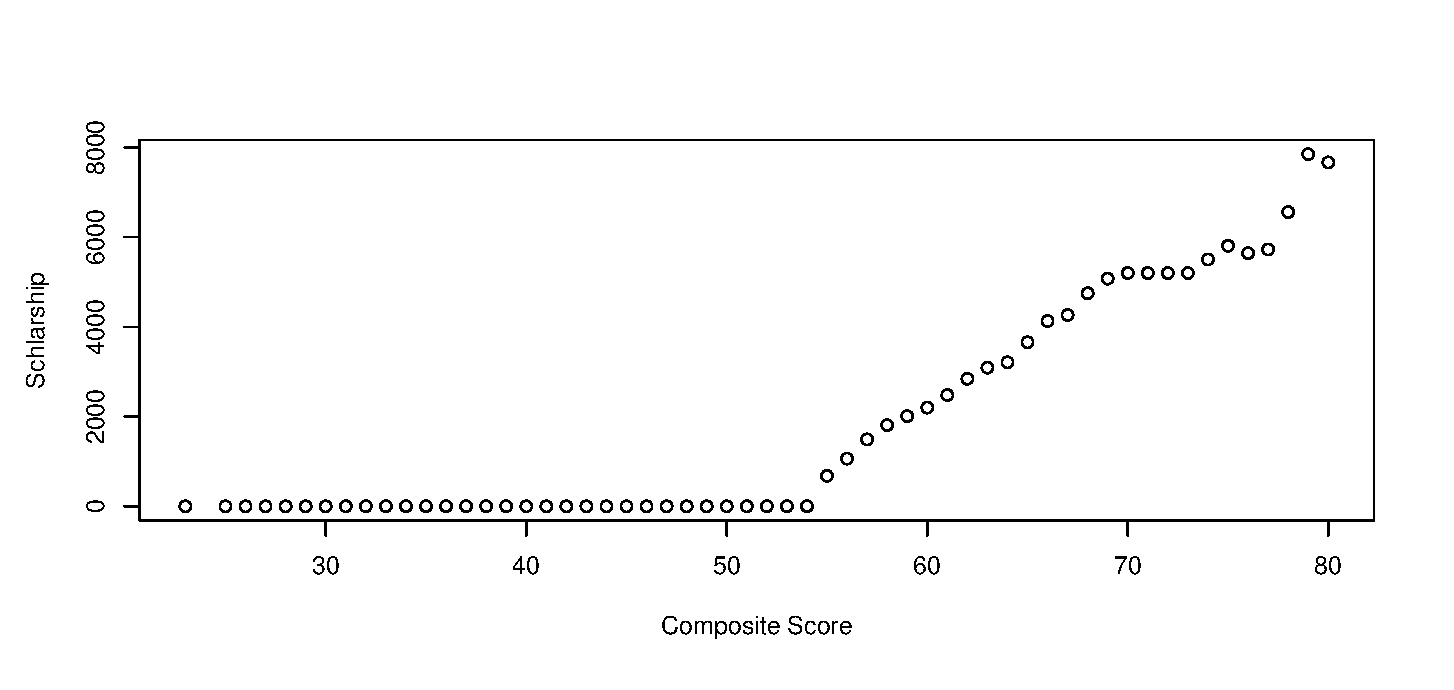
\includegraphics[scale=0.65]{pic/scho_composite.eps}
% \caption{Scholarship versus composite score}
% \label{compositescore}
%\end{figure}


\subsubsection{Stepwise Regression Based on Composite Score}
Using ``CS'' as the variable representing the composite score, a piecewise 
regression is used to capture these observations and the resulting regression 
equations are shown in Table \ref{money_result}. After the communication with 
the school enrollment administrations,  a simpler discretized version of the 
scholarship policy is shown in Table \ref{money_result_discrete}. 


% and a graph of the piecewise regression is shown in  Figure \ref{PieceWisePolicy}. 


\begin{table}[H]
\centering
\begin{tabular}{|c|c|c|}
\hline
Composite Score & \# of Applicants & Scholarship Amount \\ \hline
0-53.9         & 2,897  &0              \\ \hline
54-68.9        & 2,103  &$309\times CS -16,380 $            \\ \hline
69-76.9        &  241 &  $101\times CS - 2,024$           \\ \hline
77-80       & 19 &   $711 \times CS -48,910$          \\ \hline
\end{tabular}
\caption{Piecewise scholarship allocation}
\label{money_result}
\end{table}

% \begin{figure}[ht]
%    \centering
%  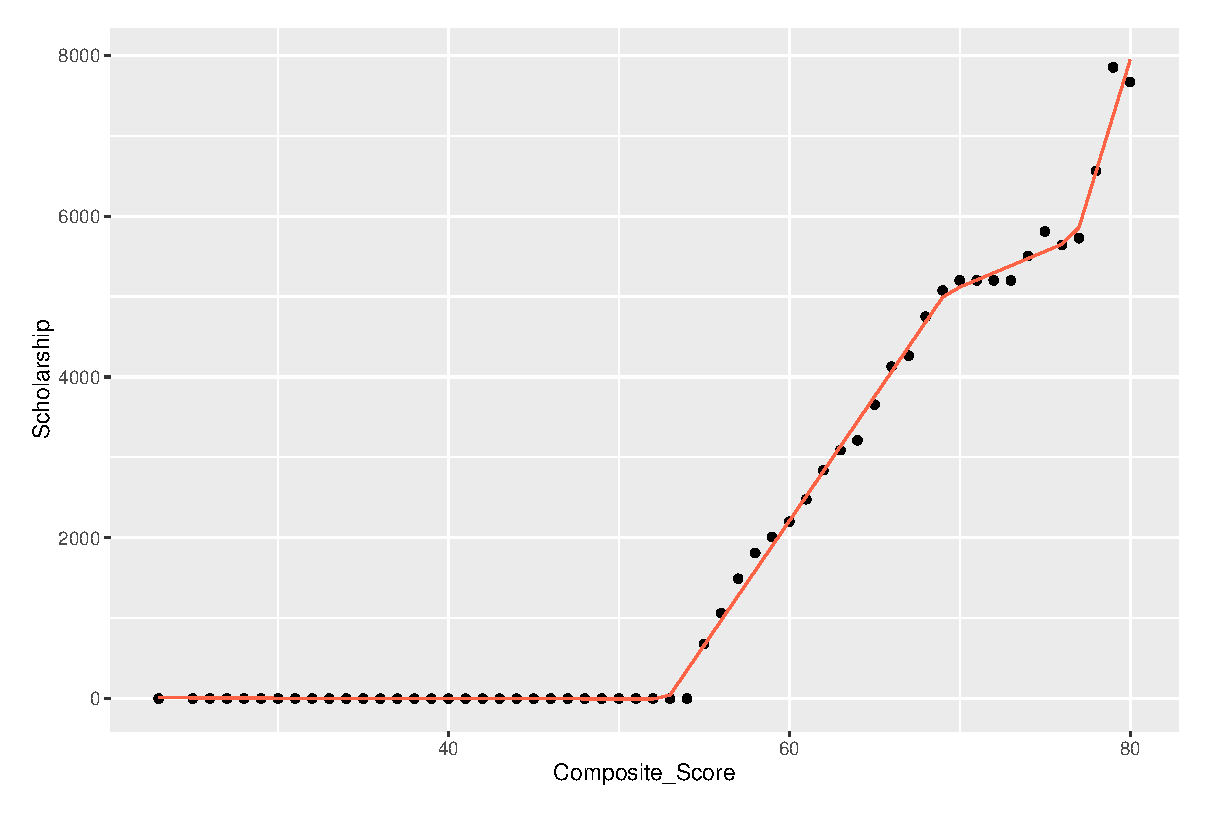
\includegraphics[width=6in, height=2.5in]{pic/PieceWiseRegression.eps}
%  \caption{Piecewise linear regression result and the original results}
%  \label{PieceWisePolicy}
% \end{figure}

\begin{table}[H]
\centering
\begin{tabular}{|c|c|} \hline
Composite Score & Scholarship Amount \\ \hline
0-54.9         & 0              \\ \hline
55-59.9         & 1,500              \\ \hline
60-65.9         & 2,500              \\ \hline
66-69.9         & 3,500              \\ \hline
70-74.9         & 4,500              \\ \hline
75+             & 6,000              \\ \hline
\end{tabular}
\caption{Discretized version of scholarship allocation}
\label{money_result_discrete}

\end{table}

\subsection{Insights on Change Of Budget}
Figures \ref{allocation_results_g}, \ref{allocation_results_h}, and \ref{allocation_results_i} show the relationship between average scholarship award and GPA and ACT for different levels of budget and different levels of SSI. Here, the horizontal axis represents composite scores, the vertical axis represents average corresponding scholarship awarded, different regression lines represent different total budgets, and different figures represent different levels of SSI.

\begin{comment}
As budget changes, the reduction of scholarship across the board seems provide the best result in all cases.
# iassac 
? the results don't seem to read that way at all, it looks like increasing budget leads to increased scholarship across the board, and increased SSI leads to smoother scholarship awards
shuai 
\end{comment}

\begin{figure} [!htbp]
\includegraphics[width=6in,height=3in]{pic/composite_10k.eps}
\caption{Scholarship vs Composite score for SSI=10,000} \label{allocation_results_g}
\end{figure}

\begin{figure} [!htbp]
\includegraphics[width=6in,height=3in]{pic/composite_12k.eps}
\caption{Scholarship vs Composite score for SSI=12,000} \label{allocation_results_h}
\end{figure}


\begin{figure} [!htbp]
\includegraphics[width=6in,height=3in]{pic/composite_14k.eps}
\caption{Scholarship vs Composite score for SSI=14,000} \label{allocation_results_i}
\end{figure}

\begin{comment}
\subsection{Comparison of Policies} 

Feeding Back these policies into the optimization model, table
\ref{policy_compare} presents the results of various policies. Here  the Objective column represents the objective values, Enrollment represents the expected enrollment; the graduation represents the expected number of graduation; tuition represents the expected tuition income, and SSI represents the expected SSI from state when applicant enroll and graduate.



    
\begin{table}[]
\centering
\caption{My caption}
\label{my-label}
\begin{tabular}{|l|l|l|l|l|l|} \hline
Policy                        & Objective & Enrollment & Graduation& Tuition &
SSI  \\ \hline \hline
Optimization Result &                 &                   &                   &
&                     \\ \hline
Decision Tree Model  &                 &                   &
&                  &                     \\ \hline
Stepwise Regression Model     &                 &                   &
&                  &                     \\ \hline
Discrete Stepwise Regression  &                 &                   &
&                  &                     \\ \hline
Current Policy                &                 &                   &
&                  &                    \\ \hline
\end{tabular}
\label{policy_compare}
\end{table}

As can be seen, it s expected that a 10\% increase in enrollment from *** to **
if we adopted the optimal result and perform individualize scholarship.  DT
tree analysis and stepwise regression and discrete stepwise regression based on
composite scores ********

Out of the composite scores, DT preforms best , followed by Stepwise 
\end{comment}


\newpage
\section{Implementation and Results}
The scholarship allocation based on the composite score and the policy presented in Table \ref{money_result} has been used as the foundation for the scholarship for the university in the 2013 to 2014 academic year.  The university has taken a proactive approach. The enrollment and admission office has purchased data on student performance and scholarship awards before they even apply (these awards hinge upon the verification of their official performance). 
%For details, please see
%\url
%{http://www.wright.edu/raider-connect/financial-aid/first-year-scholarshipsb }.

Table \ref{enroll_stats} presents the enrollment statistics for the university in the 2012 - 2013 academic year and those of the 2013 - 2014 academic year.

\begin{table}[H]
\centering
\begin{tabular}{|c|c|c|c|c|}
\hline
& 2013 & 2014 & \# Increase & \% Increase \\ \hline
Application                    & 6,101 & 6,068 & -43         & -0.7\%      \\\hline
Admitted                       & 4,541 & 4,773 & 232         & 5.1\%       \\\hline
Non-Scholarship                & 2,166 & 2,157 & -9          & -0.4\%      \\\hline
Scholarship Award              & 2,375 & 2,616 & 241         & 10.1\%      \\\hline
%\% of scholarship              & 52\% & 55\% &             &             \\ \hline
Matriculated                   & 2,001 & 2,222 & 221         & 11.0\%      \\\hline
%Non-Scholarship Student        & 931  & 1000 & 69          & 7.4\%       \\\hline
%Scholarship Student            & 1070 & 1222 & 152         & 14.2\%      \\\hline
%Scholarship Matriculation Rate & 45\% & 47\% &             &             \\\hline
\end{tabular}
\caption{Enrollment statistics for the 2012-2013 and 2013-2014 academic years}
\label{enroll_stats}

\end{table}

In 2012-2013, there are a total of 6,101 applicants; 4,541  were admitted, 2,375 were awarded scholarships, and 2,166 were not awarded scholarships. 52\% of the students were awarded scholarships, and a total of 2,001 students matriculated.

In the 2013-2014 academic year, there were a total of 6,068 applicants; of them, 4,773 were admitted, 2,616 were awarded scholarships, and 2,157 were not awarded scholarships. 56\% of the students are awarded scholarships, and a total of 2,222 students matriculated.

Notice that the number of applicants does not change dramatically, actually showing a reduction of -43 (0.7\% decrease), but the actual enrollment increased by 221  or 11.0\% over the previous years.  It is believed that the use of the optimal policy could generate millions of dollars  in revenue for the university in the next few years.

\begin{comment}
\section{Implementation}


In an attempt to improve the academic profile of our new, direct from high
school class of all 2013 and to address capacity for growth within the
colleges, the  financial aid office did a study: WSU awarded additional
scholarship funds to students who were direct admits into some colleges. The
students targeted had an average HS GPA of 3.97 and an ACT of 27+. Overall this
funding proved to be very successful because the number of students who
enrolled with a HS GPA of 4.0 and greater increased by 51\% and the students
who had an ACT of 31+ increased by 18\%. WSU matriculated an additional 34\% of
students in this group due to the additional funding.
%This effort began our scholarship leveraging efforts, and we had good results
considering the timing of the original project.
        
After an extensive data review process, we found that because the average award
for this group of students increased to \$3,500-\$4,500 (full in-state tuition
is \$8,354), WSU were able to attract higher achieving students with the
additional scholarships, by meeting their `need'\ for competitive merit-based
scholarships. WSU were competitive with our peers by percentage of tuition
discounted for this group.

We initiated the study in the 2013 Fall semester to redesign our merit-based
scholarship structure aiming to increase the headcount without sacrificing
academic profile. At the same time, a massive marketing campaign lead by the
school administration kicked off. Since more than 95\% of the incoming students
at WSU are Ohio residents, our study is focus on this group of students.

Application data from 2006 to 2013 was collected via the enrollment office. The
data contains mainly two categories: students academic profiles and economic
status. More details are included in the study approach portion of this study.
\end{comment}


\begin{comment}
\citet{Maltz2007}: developing predicting models for enrollment levels and
on systems for identifying expected targeting applicants. And the prediction
models largely consist of two levels \citet{Aksenova2006}: (1)
curve-fitting techniques such as moving averages, exponential smoothing,
spectral analysis; (2) data mining models such as regression models, tree
structure models, stochastic models.

\end{comment}

% Study on enrollment management falls into two main areas

\chapter{Conclusion}
This research studies the optimal financial aid allocation problem that puzzles many higher education institutions.  The problem is complex yet of financial importance. Various techniques have been investigated and a three-phase framework was proposed in the paper as the solution of the optimal scholarship allocation problem to derive simple yet effective financial aid policies.

In the first phase, a series of predictive models have been investigated to estimate two types of responses from students with financial aid awards. The first response is enrollment and graduation decisions from students with various socioeconomic characteristics;  the second response is the number of years of study once a student enrolls in the institution.

In the first case,  because of the binary nature of the responses,  "enroll" or "not enroll",  "graduate" or "do not graduate", logistic regression based models have been adopted to predict the probability of enrollment of an applicant and the probability of graduation given that he/she enrolls. In the second case, a regression analysis is to be used to predict the number of years of study once the student enrolls in the institution.

In the second phase, an integer linear program is designed to allocate financial aid to applicants with an objective to maximize the revenue, which is composed of tuition minus scholarship allocated over the years, plus the state share of instruction (SSI) once the student graduates.  The constraints to be observed include the total budget limitations as well as other considerations such as fairness. For a merit-based scholarship, the fairness constraint stipulates that a student with better academic performance should be assigned to an equal or higher level of scholarship than that of a students with a lower academic performance. The inclusion of the fairness constraints has dramatically increased the size of the model and a model reduction technique, referred to as minimum cardinality dominance, had to be developed to solve the model effectively.

A computational experiment shows that the use of minimum cardinality dominance has achieved a dramatic reduction regarding model size. In a test case, pairwise comparison of 6,000 students was reduced from more than 13.5 million constraints to only 191,000 constraints, enabling effective solution of the models.  In this particular case,  the original model is computationally unsolvable, actually running out of memory because of the large model size;  the reduced model nevertheless can be solved in minutes.

In the third phase, regression analysis is developed to translate the optimization results, in the form of the  amount of scholarship awarded for each student, into managerial insights and to derive a policy for implementation.  The analysis suggested that the use of a composite score, derived based on the student's GPA and ACT scores, could be used as the basis in the award of scholarships to form simple yet effective scholarship policies.

The result of the study has been successfully implemented in the exemplary state university and has resulted in millions of financial benefits.  The research would be applicable to many other institutions and offers a methodology, tools and insights into the solution of financial aid problems. 

\noindent \textbf{Future Studies.}
The results from the optimization specify the scholarship awards to each applicant under a specific population and budget.  The actual size and composition of the application pool could be affected by the unemployment rate and is random in nature.  Nevertheless, at this stage, this study is on optimization under a specific pool.  Stochastic optimization techniques such as sampling  to find the optimal allocation under a random pool will be of great interest. 

% \begin{figure}[ht]
%    \centering
%  \includegraphics[width=5.0in,height=2.8in,scale=0.5]{pic/applicant_unmployment.eps}
%  \caption{Applicants vs unemployment rate}
% \end{figure}



\begin{comment}
The response variables in the enrollment and graduation models are:
\begin{itemize}
    \item MATRICULATION. Whether the applicant enrolled or not.
    \item DEGREE.AWARDED. Whether the enrolled applicant graduated or not.
\end{itemize}

The variables represent applicant's academic performance in the model include: 
\begin{itemize}
\item GPA. The high school GPA of the applicant. The range of the GPA is 0.5 to
5. Some high school students take AP or college classes so that the GPA is
larger than 4.0.
\item  ACT. The highest ACT composite score that applicant reported. Applicant
only submit the highest ACT composite score. For student who took SAT, the
score was converted to ACT according to \citep{ACTSAT}.
\item HS.Percentile, ranging from 1 to 100, the applicant's percentile from the
high school, which is an easy way to represent applicant's standing at
graduation relative to other graduate.
\end{itemize}.    




The variables related to applicant's financial status include:
\begin{itemize}
\item TUITION. The amount of tuition that a applicant pays before the deduction
of any types of aids. Since this study does not include the out-of-state
applicants, the tuition are equal for all the applicants.
\item Family Effective Contribution (EFC). This variable is used to get the
Pell Grant information.
\item Pell Grant. The Pell Grant is converted from EFC, which followed by the
metric got from \citep{EFC_Pell}. There are 8560 applicants who did not fill
the EFC information in the data. I assumed these applicants knew that they did
qualify any Pell Grant, so that the NAs were converted to the lowest EFC which
does not qualify any Pell Grant.
\item SCHOLARSHIP. The amount amount of money applicant promised in the
enrollment stage.
\item TOTAL.FREE.MONEY. This variable is calculated as SCHOLARSHIP + PELL
GRANT. It represents that all the aids that one applicant got.
\item OUT.OF.POCKET. It is calculated as TUITION - Total.FREE.MONEY. This
indicates how much money does one applicant needs to pay.
\item UNEMPLOYMENT.INDEX. The school year Ohio unemployment rate was added to
reflect the overall economy. It is known that college is the safe harbor when
economy underperforms \citep{barr2015out}.
\end{itemize}

The personal information variables include:
\begin{itemize}
    \item GENDER. Applicant's gender.
\item HS.COUNTY.TIER. the distance between home and campus could be an important factor. This variable
relates to the distance from the county in which the applicant lived, to the university. There were six tiers in all, as well as “Out of State/Unknown”
subcategory. Tier 1 included students who lived in: Clark, Greene, Miami and
Montgomery counties. Tier 2: Butler, Champaign, Clinton, Darke, Preble and
Warren counties. Tier 3: included Auglaize, Mercer and Shelby counties. Tier 4
included Franklin, and Hamilton counties. Tier 5 was northern Ohio counties.
And Tier 6 was all other Ohio counties. As you can see, Tier 1 includes the
counties closest to the university, and Tier 5, 6/Out of State include the
counties furthest from the university.
\item HS.DISTANCE. The numeric value of distance between high school and campus
are also added.

\item ETHNICITY. This variable has several different ethnicities:
BlackOrAfricanAmerican, White, Asian, Hispanic, TwoMore.
    \item APP.COLLEGE. The intended college of a applicant.
\end{itemize}

\end{comment}

%-----------------------------------------------------------------------
% Bibliography
%-----------------------------------------------------------------------
\clearpage \phantomsection %used to correctly anchor hyperlinks
\renewcommand\baselinestretch{1.5}
%\addcontentsline{toc}{chapter}{Bibliography}
%\bibliographystyle{apalike}
\bibliographystyle{plainnat}
\bibliography{shuai_cita}


\renewcommand\baselinestretch{1.25}

\end{document}  

  
